\documentclass[twoside,12pt,a4paper]{book}

\usepackage[inner=37mm,outer=29mm,top=40mm,bottom=40mm]{geometry}
\usepackage[utf8]{inputenc}
\usepackage{minitoc}
\usepackage{natbib}
\usepackage{graphicx}
\usepackage{hyperref}
\usepackage[T1]{fontenc}
\usepackage{amsmath}
\usepackage{amssymb}
\usepackage{gensymb}
\usepackage{dsfont}
\usepackage{multirow}
\usepackage{rotating}
\usepackage[most]{tcolorbox}
\usepackage{glossaries}
\usepackage{booktabs}
\usepackage{fancyhdr}
\usepackage{algorithm}
\usepackage{algpseudocode}
\usepackage{lscape} 
\usepackage{adjustbox}
\usepackage[parfill]{parskip}
\usepackage{nomencl}
\makenomenclature

\setlength\parindent{15pt} % set indent
\setlength{\parskip}{10pt} % changes vertical space between paragraphs

\renewcommand{\arraystretch}{1.3} % Stretch a bit the table cell height

\usepackage{etoolbox}
\renewcommand\nomgroup[1]{%
  \item[\bfseries
  \ifstrequal{#1}{A}{Chapter 1-2-3}{%
  \ifstrequal{#1}{B}{Chapter 4}{}}%
]}

\DeclareMathOperator*{\argmin}{argmin}

\hypersetup{colorlinks,linkcolor={blue},citecolor={blue},urlcolor={blue}}

\setcounter{secnumdepth}{3}

% Define page style

\pagestyle{fancy}

\fancyhead[RE]{}  % right even
\fancyhead[LO]{}  % left odd
\fancyfoot[C]{\small\thepage}  % page at foot

\renewcommand{\baselinestretch}{1.1}

%%%%%%%%%%%%%%%%%%%%%%%%%%%%%%%%%%%%%%%%%%%%%%%%%%%%%%%%%%%
%%%%%%%%%%            DOCUMENT        %%%%%%%%%%%%%%%%%%%%%
%%%%%%%%%%%%%%%%%%%%%%%%%%%%%%%%%%%%%%%%%%%%%%%%%%%%%%%%%%%



\begin{document}
 \frontmatter 
\begin{titlepage}
    \begin{center}
        
        \Huge
        \textbf{Machine learning for the improvement of a blow-moulding process}
            
        \vspace{1cm}
        
        \Large  
        \textbf{Filippo CARA}
        \vspace{1cm}
        
        \large
        \begin{tabular}{ll}
            Director: & Nassim BOUDAOUD \tabularnewline
            Director: & Yves GRANDVALET \tabularnewline
            Advisor: & Amélie PONCHET-DURUPT \tabularnewline
            Advisor: & Stéphane GALLIOT \tabularnewline
        \end{tabular}
    
        \vspace*{1.5cm}
        
        \Large     
        % A thesis presented for the degree of\\
        % Doctor of Philosophy
        Thesis submitted in partial fulfilment of the requirements
        for the degree of\\
        Doctor of Philosophy
        
        \vspace{1cm}
        \includegraphics[scale=0.1]{images/UTC_logo.png}
        \vspace{0.8cm}
            
        \large
        Université de Technologie de Compiègne\\
        France\\
        November 2021
    \end{center}
\end{titlepage}

\dominitoc

\input{chapters/acknowledgements}

\chapter*{Abstract}

In the manufacturing industry, especially in the automotive sector, product quality is a major indicator for evaluating the production capacity of a company. Customers are increasingly demanding in term of product quality and providing the customer with a product that comply with the specification is essential in a market that is becoming more and more competitive. In this research work, we propose to make use of machine learning algorithms to improve the overall quality of the manufactured products in an automotive industry context. Machine learning may be used to improve the process control by better understanding how manufacturing process parameters, or features,  affect the quality of the finished part. In the same way, we claim that training a learning model able to infer in real-time the quality of a part, without any direct part measurement, could benefits to the overall quality control chain, by ensuring a fast reaction to quality deviation. Both approaches have been tested in a real manufacturing environment, the extrusion blow-moulding for fuel tank production. The experimental evaluation mainly showed two results. The first outcome has highlighted the complexity of applying data-driven methods in an industrial context where it is not possible to take into account all sources of product quality variability. Secondly, we have shown that the introduction of new sensors, such as a thermal camera at the end of the production process, made it is possible to infer in real-time some dimensional characteristics of the finished product that allows for a 100\% quality control of the produced parts.   
  
% \chapter*{Résumé}

% % Voici le résumé en français

\tableofcontents

\listoffigures
\addcontentsline{toc}{chapter}{List of Figures}

\listoftables
\addcontentsline{toc}{chapter}{List of Tables}

% \makenomenclature

\renewcommand{\nomname}{List of Symbols}

\nomenclature{\(n\)}{Number of samples}
\nomenclature{\(p\)}{Number of features}
\nomenclature{\(X \in \mathds{R}^{p \times n}\)}{General input data composed of $p$ features and $n$ samples}
\nomenclature{\(Y \in \mathds{R}^{n}\)}{Target data}
\nomenclature{\((\xi_{k}, \zeta_{k}) \in \{1,\ldots,h\}\times\{1,\ldots,w\}\)}{Pixel coordinates}
\nomenclature{\(X \in \mathds{R}^{p \times n}\)}{TO DO}
\nomenclature{\(x_{ik}\)}{Time series}



% \printnomenclature
% \addcontentsline{toc}{chapter}{List of Symbols}

\chapter*{Introduction}
\addcontentsline{toc}{chapter}{Introduction}
\thispagestyle{empty}


The development of new technologies such as Machine Learning (and Deep Learning), IoT and Cloud Computing are opening up new research perspectives in the manufacturing industry. Industry 4.0 holds the promise of increased flexibility in manufacturing, along with mass customisation, better quality, and improved productivity. In this context, Plastic Omnium Clean Energy System aims to leverage these new technologies in order to keep its leadership in the manufacturing industry of fuel tanks. For Plastic Omnium Clean Energy System, Industry 4.0 is a new way of looking at performance, with a more precise and immediate vision (based on real-time indicators) of the entire production chain, but also the optimisation of production through the use of data-driven methods. In the context of an interconnected plant, the large amount of data collected from different sources—production equipment and systems as well as enterprise—can be helpful in taking decision and contributes to a continuous improvement process. In particular, we think that the integration of machine learning models inside a complex industrial process can reduce the non-quality costs with the increase of the Overall Equipment Effectiveness (OEE). This research work will focus on the quality improvement of the fuel tanks produced through the extrusion blow-moulding manufacturing process. Extrusion blow-moulding process takes a thin-walled tube called a \textit{parison} that has been formed by extrusion, entraps it between two halves of a larger diameter mould, and then expands it by blowing air into the tube, forcing the parison out against the moulds. The fuel tank produced through this manufacturing process must respect some dimensional and geometrical constraints to comply with the customer specifications. The thickness of the tank over the whole surface must be sufficient to ensure the robustness of the part and therefore its safety, while avoiding an excessive and unnecessary weight of the finished product. Unfortunately, measuring the thickness of a hollow part is a time-consuming operation that requires several minutes of work and that cannot be done online for each part. As a consequence, only a subset of the produced parts can be measured. One set of statistical tools for applying such a screening is acceptance sampling. Using such tools enables decision makers to determine what action to take on a batch of products. Decisions based on frequency testing, rather than on 100\% inspection, are more expedient and cost effective but it cannot guarantee the conformity of all parts of the population from which the sample was drawn. In order to reinforce the control of the parts, the tank weight is measured for 100\% of the manufactured parts. The weight is an indicator of how much material is composing the part and allows for overall control of the quality of the part. Unlike the thickness, which has to be measured in several areas of the tank and cannot be carried out online for all the parts, the weight can be easily measured for all part and can provide an overall information about the amount of material composing the fuel tank. This thesis explores how data-driven methods and, in particular, machine learning and deep learning could be applied in the industrial context of the extrusion blow-moulding in order to improve the quality of the produced fuel tanks. Supervised machine learning is proposed as a tool to discover hidden patterns between the process parameters of the machine and the quality of the parts that have been manufactured.

In our opinion, the overall quality improvement of the manufactured parts could be achieved in two ways:

\begin{itemize}
    \item Through the manufacturing process optimisation.   
    \item By improving the quality control. By enhancing the quality control through a 100\% inspection of the part it is possible to react faster to quality non-conformities and to avoid to send to the customers some parts which do not comply to the specifications which may cause some Quality Recall.  
\end{itemize}
%
We claim that Machine Learning, and more in general data-driven methods, could be either used to optimise the process and the quality control. By modelling the relationship between the process and the quality data, using a data-driven method, it is possible to infer the quality of a part given a new set of input data. Moreover, by leveraging interpretable Machine Learning algorithms it is eventually possible to identify which parameters affect most the quality of the final part.    

The experimental part will be predominant in this research work. Firstly, we rely on experimentation and measurement to get all the data needed to build the statistical algorithms. The machine will be equipped with new sensors, such as \textit{RGB} or thermal cameras in order to collect a new set of previously unexplored data. These new sources of data, combined with the process data already available within the company, will constitutes the entry point for training our machine learning models. In addition, this research work has made it possible to work on a few industrial software-based applications which bring value to the overall extrusion blow-moulding manufacturing process. The development of these applications is an outcome of our work on data analysis and it constitutes a part of the contributions of this research work.

\section*{Thesis structure}

This PhD thesis is structured as follow: Chapter \ref{Industrial Context and Research Framework} focuses on detailing the industrial context in which this research work is inscribed. The extrusion blow-moulding, as well as the key quality characteristics of a fuel tank are described. Subsequently, a literature review of the quality control for the extrusion blow-moulding process is presented. This would allow for the positioning of our scientific work and to subsequently define the project objectives. Chapter \ref{Machine Learning for Quality Control} describes a general method to handle the quality improvement topic using a supervised machine learning approach. The second chapter bring also a special attention to define the core concepts and approaches used in machine learning, thus serving as an introduction to machine learning algorithms and techniques extensively used in the following chapters. Chapter \ref{From Corrective to Predictive Process Control} presents a first experimental application of the method described in Chapter \ref{Machine Learning for Quality Control}. Supervised machine learning is used  to try to infer the weight of the fuel tanks given the measured process data on the machine. This chapter will also present two software-based applications developed during the presented research work. A first application makes use of an RGB camera to measure the length of the parison in real-time. The second application allows for the optimisation of some critical phases of the machine such as the start-ups and purge cycles. In Chapter \ref{Thickness inference using thermal imaging} we show how thermal imaging, or better the surface-decay temperature, can be used to infer the thickness of fuel tanks through a learning algorithm. Three data-driven pipelines are proposed to leverage machine learning and deep learning to infer the thickness value of some critical areas. Finally, in the general conclusion we resume our contributions and  we present a few research perspectives that can be addressed in the future to push forward the research on this topic.  

\clearpage

\mainmatter

% Chapter 1
\setcounter{mtc}{3}
\chapter{Industrial Context and Research Framework}
\minitoc

In this first chapter, we present the context of the Industry 4.0 in which this thesis project is inscribed. Primarily, we will review the industry 4.0 paradigm as well as the benefits it can bring to the manufacturing industry through the application of AI-based data-driven methods. Subsequently we will describe our industrial research framework as well as the min goal of this research work: the quality improvement of the parts produced through the Extrusion Blow-Molding process. Finally, we will present what we consider to be the main contributions of our research work.

\section{Industry 4.0: a promise for improved manufacturing}

Automotive industry is nowadays driven by global competition and the need for fast adaptation of production to the ever-changing market requests. The fourth revolution in industry, Industry 4.0, holds the promise of increased flexibility in manufacturing, along with mass customisation, better quality, and improved productivity \citep{zhong2017intelligent}. As already occurred for the past three revolutions, technical innovations and a new way of perceiving the world, are radically changing the industry. The first industrial revolution at the end of the 18th century introduced steam-powered machines. The second one used electricity to improve productivity and to create mass production. Electronics and information technology, with the introduction of Programmable Logic Controllers (PLC) began the industrial automation and the third industrial revolution. The context of billions of people connected by mobile devices, with unprecedented processing power, storage capacity, and access to knowledge is promoting the emergence of new technologies. Artificial intelligence, robotics, autonomous vehicles, 3-D printing, nanotechnology, biotechnology, materials science, energy storage, and quantum computing are changing the world and today we are on the cusp of the fourth industrial revolution \citep{schwab20164th}.  

The term Industry 4.0 refers to the connection among production departments, tools, machines, “individual things” in general made possible by Internet and CPS (cyber physical systems) \citep{schlapfer2015industry} .
With the digital revolution, the boundaries between the physical and digital worlds are disappearing to create an interconnected factory with strong interactions between employees, machines and products. These connected entities can interact with one another using standard Internet-based protocols and analyse data to predict failure, configure themselves, and adapt to changes.
According to the estimations made by BCG for German companies, Industry 4.0 will have a positive impact on companies with productivity and revenue growth but also on economy with more investments and with an overall six percent increase in employment during the next ten years. Productivity improvements on conversion costs, which exclude the cost of materials, will range from 10 to 20\% in automotive industry, while productivity gains of 5 to 8\% will be achieved if the materials costs are factored in \citep{lorenz2016time}. The revenue growth, as a direct consequence of  Manufacturers demand for enhanced equipment and new data applications, as well as consumer demand for a wider variety of increasingly customised products, is estimated at 30€ billion a year, which is approximately one percent of the German GDP \citep{russmann2015industry}. 

Industry 4.0 is also a new way of looking at performance, with a more precise and immediate vision (based on real-time indicators) of the entire production chain, but also the optimisation of production through the use of artificial intelligence. In the context of an interconnected plant, the large amount of data collected from different sources—production equipment and systems as well as enterprise—can be helpful in taking decision and contributes to a continuous improvement process. In particular, we think that the integration of machine learning models inside our complex industrial processes can reduce the non-quality costs with the increase of the overall equipment effectiveness (OEE). 

In the following subsection we will present what we consider to be the two key elements that have been contributing most to the fourth industrial revolution: the Data and the Machine Learning.


\subsection{Data}

For a long time, information was documented on paper while manufacturing was realised by handicraft, therefore, the integration between information technology and manufacturing technology was neither beneficial nor feasible. Since the advent of the first electronic computer in 1940s, the rapid development of information technology (IT) has been driving manufacturing toward informatization. Since the 1960s, the development of integrated circuits has paved the way for the advancement of computer hardware and software. Since the 1980s, TCP/IP, local area network (LAN), World Wide Web (WWW), and search engine emerged one after another to meet the increasing needs for data storage, indexing, processing, and exchange. All of these information technologies were widely applied in manufacturing. As a result, many advanced manufacturing technologies were put forward, such as computer integrated manufacturing (CIM), computer aided design (CAD), manufacturing execution system (MES), computer aided manufacturing (CAM), enterprise resource planning (ERP), and networked manufacturing (NM), etc. Recently, the rise of New IT technologies such us IoT (Internet of Things) and Cloud solutions continues to provides new sources of data. Due to the deep fusion between IT and manufacturing, the degree of manufacturing smartness is progressively elevated. As a result, the manufacturing data also becomes increasingly richer \citep{tao2018data}.

As a consequence of the multitude of manufacturing technologies, industrial data comes in very different forms. This implies a lot of heterogeneity in the data which tend to complexity any data usage or comparison. Moreover, most of the data available in the manufacturing industry is \textit{Unstructured}. In this thesis we consider as \textit{Structured} any kind of data that can be stored in form of rows and columns in systems like databases or Excel Spreadsheet. Any data that can be stored by respecting this convention, without loosing any information, can be qualified as a structured data. On the other hands, we consider as \textit{Unstructured} any set of data that cannot be stored in a set of rows and columns without losing inner information. Some types of data may be difficult to definitely classify into one or the other category. It could actually depend on the use-case and the data processing objective. For example, an image can be represented as a 2D matrix (for black and white images) or as 3D matrix (for colour images). This representation is a perfectly structured. Therefore an image, or a video, could be considered as a structured data format for someone willing to conduct a spectral analysis, only interested in the pixel values and positions. Nonetheless, the same image can also be considered unstructured if we focus our interest on the content of the image. Indeed, pixel values can not be easily translated into a structured representation of the actual content.
Nonetheless, someone willing to extract design intents from these files will probably argue a different point of view considering the difficulty to access this implicit information. Moreover relying on hypothetical metadata, with varying quality and content, can not be considered as a viable systematic solution to this problem, therefore justifying that many engineering standardised formats could, in fact, be considered as unstructured data formats, under specific objectives, despite being implemented in perfectly structured and standardised data formats.

Unfortunately, dealing with unstructured data is a lot more challenging in a data science perspective \citep{blumberg2003problem}\citep{sagiroglu2013big} \citep{buneman1997adding}. It requires highly complex, expensive and time-consuming feature extraction processes and operations (i.e. a feature represents a descriptor (e.g. colour of a car) in a data science context). It is estimated that the average \textit{Information Systems} (IS) roughly contain around 15\% of structured data and 85\% of unstructured data. Such an assumption seems consistent with the actual status of the manufacturing industry. Furthermore, even if a more optimistic situation is considered, with a balanced rate of 50\% structured and 50\% unstructured data, it still appears critical to be able to mine, explore, exploit, and search in these data. Consequently, we could state that a Big Data context is inherently linked to unstructured data.
Dealing with manufacturing data implies to use and manage large amounts of human-made data. These data come with inherent and recurring issues which highly limit their usability without an extensive pre-processing.

\subsection{Machine Learning and Deep Learning}

As highlighted before in the previous section, the amount of available data is exponentially increasing and thus it can be reasonably considered that humans will not be able any more, in a near future, to process, by hand, these massive amounts of data and perform heavy computations in a parallel manner. Nonetheless, software products based on Machine Learning algorithms, take advantage of parallel computation capabilities and large data quantities to approach human behaviours and understanding in complex situations. Machine Learning, and more generally data-driven methods, introduce a new way to deal with manufacturing problems. Unlike traditional methods of rule-based or mechanism-based modelling, one of the major advantages of data-driven industrial technology is the ability to establish predictive analysis based on insight and evidence contained in the data, which allows for establishing smart management tools for invisible problems and exploring the relationships between complex things. This way, new knowledge is accumulated to form an intelligent system which can be continuously iterated on.

In last decade, the hottest machine learning sub-field, Deep Learning has gained a lot of popularity due to the ability to provide state-of-the-art results in multiple domains: from web searches, to image recognition and detection through Convolutional Neural Networks, to natural language processing with Recurrent Neural Networks and, more recently Self-Attention based Neural Networks. Deep Learning is not a new idea, most of the recent proposed Deep Learning architectures are built using discoveries from the last years of the 20th century. Deep Learning has received new attention again in 2012 when Alex Krizhevsky and his colleagues used deep learning technology \citep{krizhevsky2012imagenet} on ImageNet for the first time to outperform other teams in an image classification task, making people aware of the advantages of deep learning over traditional machine learning, bringing deep learning to the forefront for the first time. The reborn popularity of these computational methods can be attributed to the following reasons:

\begin{itemize}
    \item \emph{Increasing Computer Power}: GPU (Graphical Processing Unit) computing enabled, in the early 2010s, improved calculation performance in the field of Machine Learning. Powerful, fast and cheap GPU-devices are some of the devices which greatly helped researchers to reach performances never achieved before, especially in the Machine Learning (ML) field dedicated to the study of deep Neural Network: Deep Learning (DL). Deep learning involves huge amount of matrix multiplications and other operations which can be massively parallelised and thus sped up on GPUs.
    \item \emph{Larger labeled datasets}: The explosion of Big Data in the last decade, has considerably increased the size of the dataset available inside the manufacturing companies. The availability of an important amount of data is indispensable for the successful application of Deep learning methods because these methods require, in average, more data compared to conventional Machine learning approaches. For instance, the ImageNet dataset \citep{deng2009imagenet} released in 2009, contains more than 14 millions images, with the corresponding labels, which can be used for training image classifiers models.
    \item \emph{Advances in Deep Learning research}: Deep Learning is one of the most popular research topics of the moment and interest in this area is growing every year. As pointed by the "AI index 2019 report" \citep{zhang2021ai}, between 1998 and 2018, the volume of peer-reviewed AI papers has grown by more than 300\%, accounting for 3\% of peer-reviewed journal (Figure \ref{fig:Number of Peer-Reviewed AI Publications}) publications and 9\% of published conference papers. This increase in the number of researchers leads to faster research progression. 
    \item \emph{Open source tools and models}: The democratisation of open sources frameworks such as \textit{PyTorch} \citep{paszke2019pytorch}, \textit{Tensorflow} \citep{tensorflow2015-whitepaper}, \textit{Keras} \citep{chollet2015keras} and \textit{Scikit-Learn} \citep{scikit-learn} allow to apply Machine Learning and Deep learning methods with a few line of code. Moreover, the Machine Learning community is rather open in sharing results. There exist a lot of pre-trained models available online which can be used as a starting point for \textit{Transfer Learning} (\ref{Transfer Learning}).  
\end{itemize}

\begin{figure}
\centerline{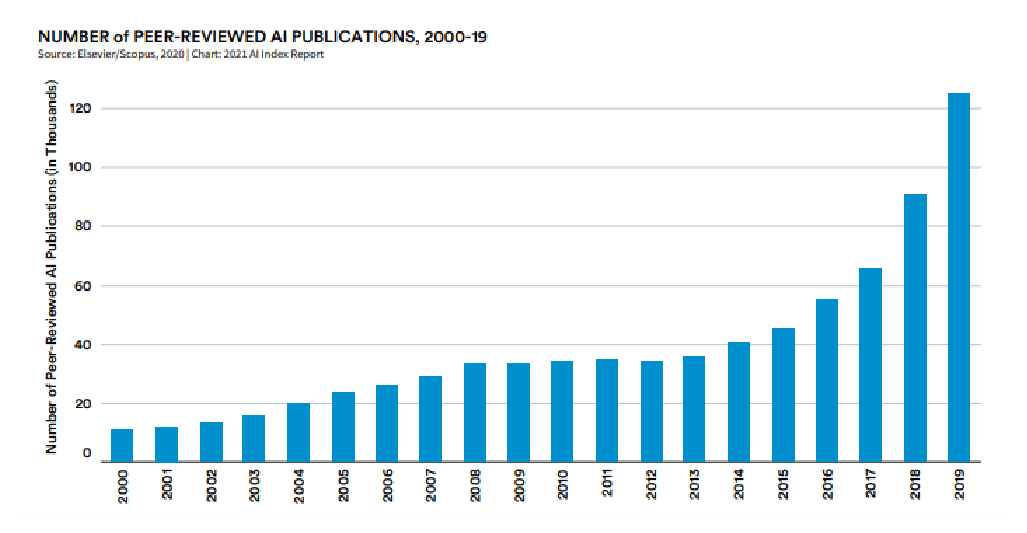
\includegraphics[scale=0.9]{images/chapter_1/AI_report.eps}}
\caption{Number of Peer-Reviewed AI Publications, 2000-2019 \citep{zhang2021ai}}
\label{fig:Number of Peer-Reviewed AI Publications}
\end{figure}


\subsubsection{Review of opportunities for the manufacturing industry}

In this section, we presents the result of a literature review we conducted to highlight some of the possibles applications where the Machine Learning could be applied in order to create value for the manufacturing companies. This study should not, in any case, be considered as an exhaustive list of possibilities. Results are summarised in table \ref{tab:ai_benefits}. 

\begin{table}
\label{tab:ai_benefits}
\begin{tabular}{|l|p{6cm}|p{4cm}|}
\hline
%
Domain &
  Benefits &
    Bibliography \\ \hline
% Quality Optimization
Quality Optimisation &
  Decrease the product failure rate at the end of the production line. Optimize key performance index of the final product to meet customer needs. &
    \citep{lieber2013quality, li2018ensemble, chen2008neural, nagorny2017quality, haeussler1996quality} \\ \hline

Maintenance &
  Increase the availability of the production line by preventing the breakdown of equipment in advance. Predict the risk of malfunction of the production line and arrange proactive maintenance. &
    \citep{nguyen2019new, lee2017application, einabadi2019dynamic, li2017intelligent, liu2016prediction}\\ \hline
Fault Diagnosis &
  Prognostic diagnose of production line failure event. Identify the malfunction part of the production line. Predict the abnormal behaviors of machines and equipment. & \citep{toma2020bearing, wong2006modified, chen2014fault, malik2017artificial, arabaci2010automatic} \\ \hline
Scheduling Optimisation &
  Logistic management of the production line, which can maximize the throughput of the production line. Buffer control and product routing management. & \citep{morariu2020machine, woschank2020review, lolli2019machine, zhang2019review, gomes2016developing} \\ \hline
\end{tabular}
\caption{ML opportunities in Manufacturing}
\end{table}

\subsubsection{Challenges of AI in Industry}

Although AI technology has made breakthroughs in many applications, there is still a big gap between large-scale usage in industrial scenarios. This is because industry and manufacturing value stability, standardisation, accuracy, and repeatability, as well as mechanisation, processes, operations, and close integration of process requirements \citep{lee2020industrial}. Before AI technologies can be fully integrated into industrial systems, it is necessary to overcome the challenges of reproducibility, reliability, and security

\paragraph{Reproductibility}

% TO REVIEW

Unfortunately, this practice is not widely adopted by researchers in the manufacturing research
communities. Too few datasets are actually available to conduct research. It can be assumed that
the lack of opened datasets is probably induced by the secretive policies frequently enforced in the manufacturing industry. Unfortunately, this tends to hinder research possibilities and produce the following unwanted side-effects:

\begin{itemize}
    \item Very difficult, if not impossible, to reproduce any claimed result in the state-of-the-art. This highly limits the effectiveness of peer-reviewing.
    \item Very difficult, if not impossible, to compare the proposed approaches to address a specific problem. Aside of qualitative studies, there is no common metric based on a shared dataset to evaluate and rank the different methods.
    \item Developing a dataset may literally cost millions of dollars. If every researcher or research group needs to build a new one from scratch, the developing costs will be are multiplied.
    \item Small research laboratories may not be able to work on some research topics due to a lack of funds available to build a decent dataset. This situation may namely affect the emerging countries.
\end{itemize}



\paragraph{Data issues}


Concerning data, AI technology out the manufacturing industry faces five major challenges and limitations: 

\begin{enumerate}
    \item Training data is heavily dependent on manual work, otherwise it is difficult to obtain a large and comprehensive training data set, and the quality of labeling is heavily dependent on human experience and ability.
    \item The transparency of the model needs
    to be improved since AI algorithms cannot explain how conclusions are reached step-by-step.
    \item Models are not very general, and it is hard to replicate from one application to the next. This means lots of money and energy is needed to train new models for new problems.
    \item The risk of deviation in data and algorithms, much
    like the differences between societies and culture, requires extensive steps to solve.
    \item It is difficult to reach agreement on data privacy and attribution.
\end{enumerate}

\paragraph{Reliability}

% TO REVIEW

According to the different requirements of reliability in different domains and applications, AI can be roughly divided into mission-critical and non-mission-critical applications. Currently, most AI products on the market do not require strict system reliability. As long as a certain threshold of usability is reached, the occasional errors and problems can be tolerated without serious consequences in non-mission-critical applications. For critical applications, if a system has even a small chance of failure, it could lead to serious consequences, causing property loss or even harm to human beings or social stability. This is particularly true for all those applications that have to do with the safety of people. An example of this is the intelligent driving industry: it is expected
that this industry will globally reach \$9.5 billion by 2020. The industry is facing serious challenges in guaranteeing safety. The first fatal drone crash occurred in March of 2018, and an Uber autopilot test car hit and killed a woman in May of 2018. Whether it is true autonomous driving technology or a driving assistance system, its high demand for reliability and intolerance of failures makes it difficult for the technology to truly enter the market before exceeding the human driving level. These challenges are the same in industrial systems. If we want to employ AI technology to control the functioning of an entire system, we must be extremely cautious about mission-critical tasks, which necessitates not just advancements in model and algorithm accuracy, but also security limits and uncertainty management in system design. For instance, for a manufacturing company with low percentage of quality scraps, an AI model with a 80\% accuracy in prediction may lead to incorrect alerts FINIRE 


\section{The research framework: The Extrusion Blow Molding}


The industrial process taken into account for our experimental setting is the Extrusion Blow-Moulding process. Extrusion blow molding is a process used to form hollow thermoplastic objects (especially bottles and containers). The process takes a thin-walled tube called a \textit{parison} that has been formed by extrusion, entraps it between two halves of a larger diameter mold, and then expands it by blowing air into the tube, forcing the parison out against the mold. The outside of the thin-walled part takes the shape of the inside of the mold \citep{poli2001design}.

\begin{figure}
\centerline{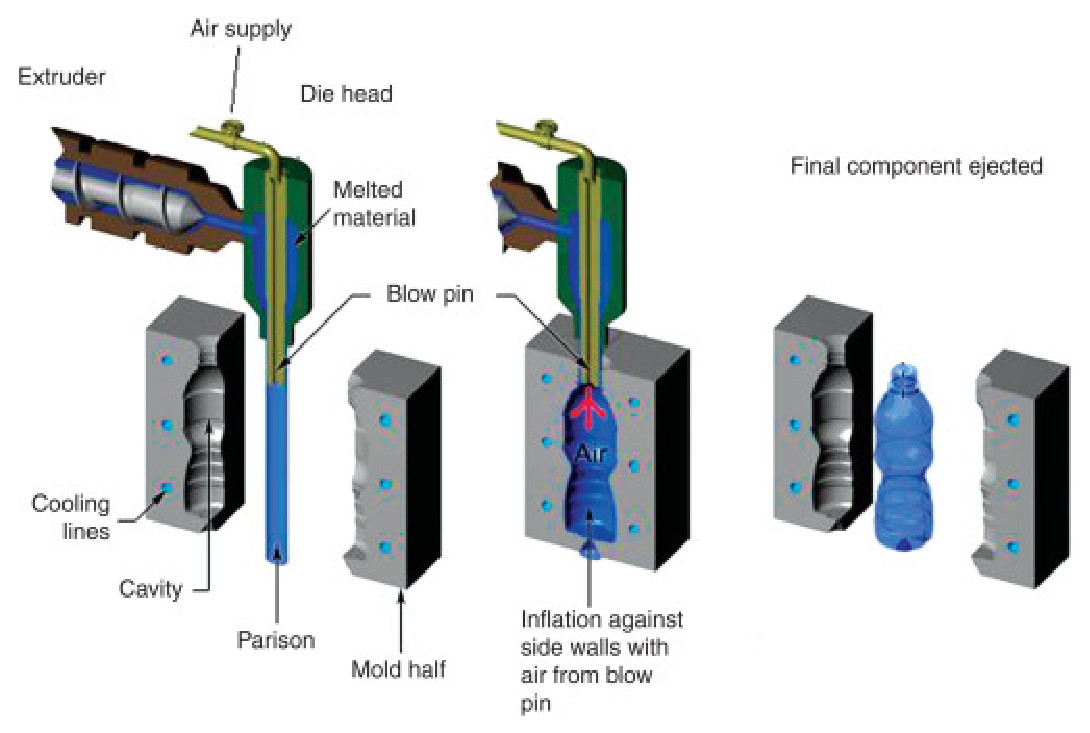
\includegraphics[scale=0.75]{images/chapter_1/extrusion_blow_molding.eps}}
\caption{Extrusion Blow-Molding \citep{goodship2015design}}
\label{fig:Extrusion Blow-Molding}
\end{figure}

As easily guessed by the name, the Extrusion Blow-Molding process is composed of two sub-processes: Extrusion and Blow-Molding.

\begin{itemize}
    \item \textit{The Extrusion:} The Extrusion is a continuous-flow process where a plastic material feedstock is fed through a hopper onto a feeding transfer screw. The thermal energy provided by the heating clamps as well as the mechanical energy provided by the screw rotation allow the melting of the plastic material.The die will typically create a tubular extruded cross-section, round or oval depending upon the final shape of the finished blow molded part. The melt is extruded through an annular die of adjustable gap, to form a hollow cylindrical membrane known as a parison. The die gap is the distance between the inner mandrel and the outer bushing. The gap can be varied during the extrusion, due to the tapered nature of the die, by moving either the mandrel or the bushing in a vertical direction. The process of variable die gap extrusion is referred to as parison programming and is utilised to manipulate the thickness distribution in the final part \citep{diraddo1993profile}.
    \item \textit{The Blow-Molding:} Unlike Extrusion, Blow-Molding is a discontinuous-flow process. In extrusion blow moulding, the parison is vertically suspended in the air during which time two mould halves enclose it by the action of a pneumatic or hydraulic mechanism. Internally applied air pressure causes the parison to inflate and take the shape of the inner parts of the molds. Once the blow operation is completed and the part has frozen suitably for ejection, the mold opens and the part is ejected, allowing the extruded parison to be extruded through the mold for the next cycle. 
\end{itemize}

Each phase has parameters that influence the subsequent phases and, ultimately, the characteristics of the finished product. The multiple phases mean that the number of parameters that can be adjusted on the process is fairly high. It is possible to fine-tune temperatures, screw speeds and throughputs for the Extrusion, as well as the  pressure curves, molds opening and closing times for the Blow-Molding phase. In addition, the Extrusion Blow-moulding process has a certain dynamic: it takes a certain amount of time for the adjustment of one of the process parameters to have an effect on the products. This dynamic is mainly due to the thermal inertia of the solid tooling.
One of the most critical part of the process is the parison formation. In fact, the dimensions of the blow molded article are directly related to the dimensions of the parison. Furthermore, the thermo-mechanical history of the material during the parison formation stage and the resulting weight and diameter distribution of the parison have a great influence on the characteristics of the subsequent inflation and cooling stages. The shape and the dimensions of the parison are the result of complex interactions between the molten ploymer and the thermo-mechanical conditions that influence the melt after it leaves the extruder die. Parison formation it is affected by two phenomena knows as \textit{swell} and \textit{sag}. Parison swell, occurring both in diameter and thickness, is due to the nonlinear viscoelastic deformation of the polymer melt in the extrusion die. Sag is caused by gravitational forces that act on the suspended parison \citep{huang2002prediction}. A high degree of swell could lead to molded articles which are to heavy and uneconomical, on the other hands, very low swelling could yield incomplete parts of low weight with unacceptable wall thickness.

There are many variations of this process including equipment made to extrude multiple parisons simultaneously, equipment that can extrude multiple layers within the same parison, equipment with rotary capability that will hold several molds and can provide a continuous nonstop process. Moreover, the extrusion blow-molding process can be split into two subcategories: intermittent extrusion blow molding and continuous extrusion blow molding. With intermittent extrusion blow molding, the extruder runs for a designated amount of time and fills a reservoir with plastic. Once the the reservoir has been filled, a plunger is activated and pushes the material from the reservoir through the extrusion head. On the other hand, in continuous blow-molding, the plastic is extruded permanently in a continuous manner while the machine runs.

In the context of this thesis project we have mainly worked with a continuous Extrusion Blow-Molding process, whose finished products are obtained from the overlay of multiple plastic layers. This particular type of Blow-Molding process takes the name of \textit{Co-extrusion}. Co-extrusion was born out of the need of reduce the permeability of fuel tanks. The steps for producing a multi-layers plastic product are the same as those used by the traditional single layer process, except for the number of extruders involved in the manufacturing process. Up to six extruders can be used simultaneously to melt different plastic materials. The goal is to create a multi-layer tank with the use of different material, as shown in
Figure \ref{fig:Co-extrusion Process}

\begin{figure}
\centerline{\includegraphics[scale=0.55]{images/chapter_1/coextrusion.png}}
\caption{Co-extrusion Process}
\label{fig:Co-extrusion Process}
\end{figure}

The Extrusion Blow-Molding constitutes one of the various stages necessary to produce the finished part. The stages needed to manufacture a finished part may vary depending on the type of product made. For instance, a fuel tank container, a plastic bottle or a plastic bumper may requires different post-production processes. Further information on how a fuel tank is produced are available in Appendix \ref{Full production process}. As far as our thesis work is concerned, we will only focus on The Extrusion Blow-Molding stage.


\subsection{The key parameters of the Extrusion Blow-Molding} \label{The key parameters of the Extrusion Blow-Molding}

The following table resume the list of the key parameters of an extrusion blow-molding process.

% Put table in landscape view
\begin{landscape}
\begin{table}[]
\caption{Blow-Molding Key parameters}
\label{tab:key_parameters}
\begin{tabular}{|l|l|l|l|l|l|}
\hline
Process      & Parameter            & Unity of measure & Value range   & Description                 & Dependencies \\ \hline
Extrusion    & Speed*               & RPM              & {[}0, 90{]}   & Rotation speed of the screw &              \\ \hline
Extrusion    & Throughput*          & Kg/h             &               &                             &              \\ \hline
Extrusion    & Feeding Temperature* & °C               &               &                             &              \\ \hline
Extrusion    & Melt Temperature*    & °C               &               &                             &              \\ \hline
Extrusion    & Cycle time           & s                & {[}60, 120{]} &                             &              \\ \hline
Extrusion    & Parison profile      &                  &               &                             &              \\ \hline
Blow-Molding & Blowing pressure**   &                  &               &                             &              \\ \hline
Blow-Molding &                      &                  &               &                             &              \\ \hline
Blow-Molding &                      &                  &               &                             &              \\ \hline
\end{tabular}
\end{table}
\end{landscape}

\subsection{The Quality of an extruded blow-molded part}

Quality Control is generally expressed as a management activity verifying the conformity of the process and the product/service to the requirements that constitute its quality standard. The ISO 9000 standard defines quality control as "A part of quality management focused on fulfilling quality requirements". In the industrial context taken into account the requirements are defined by the customers. Several characteristics are measured on the product and compared with the customer requirements, if the measures are compliant with the customer specifications the part can be sent to the customer, otherwise the part have to be rejected. 
In the framework of the Extrusion Blow-Molding process, we are mostly interested in the dimensional/geometric characteristics. In fact, 


The following table resume some of the specific tests that have to be carried to the blow-molded parts to ensure their conformity to the customer specifications.


\begin{table}[]

\caption{Quality tests}
\end{table}


% Insert Blow-Molding table

\section{Main objective}

Because manufacturing processes are becoming more and more complex, and the high level of requirement in the automotive industry regarding safety and environmental impacts, Plastic Omnium is continuously seeking for innovation throughout its different projects that allows the company to remain leader in its field. For Plastic Omnium, the Industry 4.0 paradigm can provide a new way of looking at performance, with a more precise and immediate vision (based on real-time indicators) of the entire production chain, but also the optimisation of production through the use of data-driven methods. An in-depth presentation of the activities of Plastic Omnium is available in Appendix \ref{Plastic Omnium}.

For Plastic Omnium the are four main pillars of the 



\begin{figure}
\centerline{\includegraphics[scale=0.50]{images/chapter_1/Digitalisation_pillars.png}}
\caption{Industry 4.0 pillars for Plastic Omnium}
\label{fig:pillars}
\end{figure}


Among the different topics, this research work will focus on the Quality topic.
For an equipment manufacturer like Plastic Omnium Clean Energy Systems, bad or ``scrap'' parts are very expensive for the company. The “Cost of Non-Quality” (CNQ) is one of the key indicators most used by the company. 



Using the data that is already available within the company will be an important part of the global study, because it will be the first input going into the developed monitoring system. In the case of Plastic Omnium CES, the data coming from the systems "PES" and "DASIP" will be important. The two systems allow the traceability of the produced parts as well as a monitoring of the different events happening on the plant’s machines (for PES), and DASIP is monitoring key parameters of the production processes. Other data sources will be investigated during this work.

To reach the final objective of reducing the scraps and the non-quality costs, a methodology will be proposed in order to implement a predictive system. This methodology will include both the requirements to solve the industrial and scientific issues discussed in the next part. A phase of validation and performance analysis of the proposed approach is also required, to ensure its relevance in the industrial context, and its interest compared to other approaches of the literature.

Previous works focused mainly on two themes: Process optimisation and Quality monitoring.  


\section{Contributions: Towards new quality control framework}

Our dissertation develops along two major axes: the process improvement and the quality control improvement. We claims that the improving of the overall quality of a production line can be obtained by working either on the process and either on the quality control. This for us definitely makes sense as the production of a part compliant with the specifications is the result of a careful work in optimising the production process, as well as the ability to quickly identify a deviation in the quality of the finished part. By quickly identifying a quality problem it is possible to react faster and adjust the process, limiting the production of non-conforming parts.

This thesis has, in our opinion three main contributions:

\begin{enumerate}
    \item It provides a general framework to improve the Process Control of a complex manufacturing process. We propose a data-driven approach which take advantage of the historical data to try to model the relationship between process parameters and the quality of a product. The approach presented in chapters 3 aims to leverage the information available in the large amount of data collected in the manufacturing process 
    
    Our approach, presented in Chapter 3 is composed of 4 main stages: the data acquisition, the data processing, the Machine Learning modeling and the FINIRE. The four stages 
    \item It provides a general framework to improve the Quality Control. Using a data-driven approach we can use sensors, cameras or any kind of equipment to collect meaningful data. This approach open ups new possibilities in term of Quality Control.  
    \item In Chapter 4, we propose an approach to infer the thickness of Blow-Molded parts using thermal imaging and a Deep Learning without any direct measurement of the part. We claims that this    
\end{enumerate}


\section{Conclusion}

In this first chapter we have highlighted the context in wh

\subsection{Scientific Contribution}

\subsection{Industrial Contribution}

In this chapter we have seen that we are on the cusp of the 4th industrial resolution. Industry 4.0, holds the promise of increased flexibility in manufacturing, along with mass customization, better quality, and improved productivity. The development of new technologies such us the AI, the IoT are opening up new perspective in the Manufacturing Industry. AI in particular seems able to take advantage of the fast growing amount of data available in the manufacturing plants to FINIRE 


% Chapter 2
\setcounter{mtc}{4}
\chapter{Machine Learning for Quality Control} \label{Machine Learning for Quality Control}
\minitoc

\section{Introduction}

Recent advancements in Machine Learning in the last few decades have opened up new research perspectives in the quality monitoring domain. In this chapter, we describe a general framework that can be applied to model the relationship between machine process data and product quality. The described methods relies on four consecutive stages: data acquisition, data processing, exploratory data analysis and supervised machine learning modelling. The application of such a method could bring a few major benefits to the manufacturing company: on one side, it would allow for a better understanding of which process parameters have an important influence on finished parts quality. In such a way, it is possible to put them under close monitoring to ensure their stability over time. Moreover, the trained model could be used to infer part quality given a new set of input process data. In such a way it is possible to provide a quality status to each part produced. This is particularly interesting every time that a quality control cannot be performed on all part produced. In fact, most companies cannot test every single product. There may simply be too high a volume or number of them to inspect at a reasonable cost or within a reasonable time frame. Or effective testing might result in the destruction of the product or render it unfit for sale in some way. By providing the quality status for 100\% of the part produced it is possible to react faster to quality non-conformities and to avoid sending to the customer a part which is non compliant with the specifications.  In the second part of the current chapter, we also bring a special attention to define the core concepts and approaches used in Machine Learning, thus serving as an introduction to Machine Learning algorithms and techniques extensively used in the other chapters of this PhD dissertation.

\section{Towards data-driven quality control}

In the manufacturing industry, product quality is an indicator for evaluating the production capacity of a company. Customers are increasingly demanding in terms of product quality and providing the customer with a product that complies with the specifications is absolutely essential in a market that is becoming more and more competitive. The best possible solution to deliver 100\% of compliant parts to the customer would be to inspect in details all parts produced. However, most companies cannot test every single product. There may simply be too high a volume or number of them to inspect at a reasonable cost or within a reasonable time frame. Or effective testing might result in the destruction of the product or render it unfit for sale in some way. In our industrial context, the quality control is a time-consuming operation that requires several minutes of work and that cannot be done online for each part. As a consequence, only a subset of the produced parts can be measured. One set of statistical tools for applying such a screening is acceptance sampling. Using such tools enables decision makers to determine what action to take on a batch of products. Decisions based on frequency testing, rather than on 100\% inspection, are more expedient and cost effective but it cannot guarantee the conformity of all parts of the population from which the sample was drawn~\citep{fuchs1998multivariate}.
% In this section, we extend the concept that was presented in Chapter \ref{From Corrective to Predictive Process Control} in order to develop a general framework for inferring the quality of a manufactured part without directly measuring it. One more time, we will take advantage of machine learning ability to learn the transfer function from some input data to the product quality. The trained model could then be applied to enhance manufacturing quality control by providing a quality status to the part.
Figure \ref{fig:statistical_quality_control} outlines the functioning of acceptance sampling. 

\begin{figure}
\centering
\includegraphics[scale=0.50]{images/chapter_4/statistical_quality_control.png}
\caption{Statistical quality control}
\label{fig:statistical_quality_control}
\end{figure}

Although this method is widely applied in the manufacturing industry and it is globally accepted, it presents three major drawbacks:
\begin{enumerate}
    \item The acceptance sampling method is able to track deviations in product quality, but it is not able to provide 100\% quality inspection. As a result, it may happen that one or multiples non-compliant parts are produced, as a response to a temporary malfunction in the production process, and these parts may not be detected. This may result in one or multiple non-compliant parts being sent to the customer.
    \item The second drawback of Acceptance Sampling is the delay in detecting a process deviation. If product quality starts to deviate, the manufacturer has to wait for the next quality control to identify the problem and to be able to act on the process to correct it. Moreover, parts produced in this time frame are potentially non-compliant and extra time-consuming quality control may be required to establish whether or not the parts can be sent to the customer.
    \item Another problem to consider, is the one related to the destruction of the pieces being measured. In fact, some quality measurements involve the destruction of the part or some modifications that make it unsuitable for sale to the customer. For instance, advanced quality control for assessing material distribution of each thickness layer of a blow-moulded part requires the cutting of the piece in small samples, subsequently analysed in the laboratory. Even if these tests are necessary and important to certify partconformity, it constitutes a source of waste for the manufacturer, increasing the number of PPM (parts per million) defects.
\end{enumerate}
%
In order to improve quality control of the parts, we propose to perform a comprehensive quality control using a machine learning based approach. The idea is to infer the quality status of each part produced through the use of a machine learning algorithm. The approach would be described in details in the following sections of the current chapter. 
In the context of this PhD study, the approach of inferring part quality using a trained machine learning algorithm is called \textit{data driven model-based quality control}.
The benefits that this approach can bring to quality control throughout the manufacturing industry are manifold. First, it ensures a quality control on all parts produced which enable for a fast reaction to quality non-conformities (Figure \ref{fig:model_quality_control} on the left side). In fact, by ``virtually'' measuring each part, we are able to eventually discard parts for which the model has provided a ``Not-OK'' result, or request the quality team to carry out more in-depth tests. Model-based quality measurement may be effectively used to detect those parts that turn out to be, from a statistical point of view, outliers. In this way, instead of randomly sampling the parts to be measured by the quality operators, the model is able to suggest parts that seem to be interesting.
By discarding all non-compliant parts, this approach indirectly reduces product recalls and thus the whole series of requests to return, exchange or replace a product that has been found to be defective, and which could impair performance, harm consumers or cause legal problems for producers.

\begin{landscape}
\begin{figure}
\centering
\includegraphics[scale=0.50]{images/chapter_4/data_driven_model.png}
\caption{Data-driven model-based quality control}
\label{fig:model_quality_control}
\end{figure}
\end{landscape}

If the trained model is sufficiently robust and accurate at predicting the quality status of a part, a second stage would be to reduce the real quality controls which destroy the parts or make them unusable (Figure \ref{fig:model_quality_control} on the right side). In such a case, not only the model-based control would be able to provide a thorough quality control, but it would also be able to reduce the scraps which account for an overall better production performance. Of course, real part measurements cannot be completely replaced by model-based measurements. In fact, real measurements are the primary data source to train the data-driven model. 


\section{Proposed method} \label{Proposed Method}

In this section, we will try to describe a general framework that can be applied to improve process control. We use supervised machine learning to discover some patterns between process parameters and part quality that has been manufactured by the same process. We proceed in four main stages:
\begin{enumerate}
    \item \textit{Data collection} consists in retrieving all the data needed to model the manufacturing production process. It involves two main stages:  data acquisition and  data labelling (Section \ref{Data Collection}). 
    \item \textit{Data processing} covers the range of operations required to make the input data suitable for the machine learning algorithm (Section \ref{Data Processing}). 
    \item \textit{Exploratory data analysis} is an ensemble of graphical and quantitative techniques that can be used to explore data and retrieve important information (Section \ref{Exploratory Data Analysis}).
    \item \textit{Data modelling} corresponds to the statistical modelling of the relationship between the process data and the quality data by a machine learning algorithm (Section \ref{Machine Learning modeling})
\end{enumerate}

In the remaining part of the current section we will review in details how to carry out these four steps to achieve a \textit{predictive process control}. 

\subsection{Data collection} \label{Data Collection}

Collecting data allows to capture a record of past events so that we can use data analysis to find recurring patterns. In the context of this research work, data collection is the task of retrieving the data that could be meaningful to explain the variability of a quality characteristic given some process parameters. Among the many challenges in Industry 4.0, data collection is becoming one of the critical bottlenecks. It is known that the majority of the time for building end-to-end data-driven models is spent on preparing data, which includes collecting, cleaning, analysing, visualising, and feature engineering. Moreover, as machine learning is used in new applications, it is usually the case that there is not enough training data. Traditional applications of machine learning like machine translation or image object detection rely on huge quantities of training data that have been accumulated for decades. On the other hand, more recent applications, especially in the manufacturing industry, have little or no training data. To train a machine learning model, it is necessary to have samples that are representative of the entire operating range of the process. If the individuals do not cover the whole process functioning, the model will be biased.

Two kind of data are required: input data, corresponding to the process data and output data which is actually the measurement of the part quality. Data collection involves mainly two different steps: \textit{process data acquisition} and \textit{Quality data acquisition}. 

\subsubsection{Process data acquisition} \label{Process Data Acquisition}

We use here the term \textit{process data} for any type of data belonging to the manufacturing process. For instance, some process data of the extrusion blow-moulding process are extruder throughputs, extruder temperatures, or blowing air pressures. This process data is a picture of the process state at a given time.

Process data acquisition is a challenging task in Industry 4.0 due to different technologies, machines, sensors, IoT devices and communication networks. Sensors, actuators, and Programmable logic controllers (PLCs) are the main data generators in the automotive industry \citep{khan2017big}. In the last decade a new type of intelligent sensor, also called \textit{smart sensors}, is more and more used in the manufacturing industry. Most of the data available in the Manufacturing plants comes from PLCs, sensors and smart sensors. The three devices are further explained as below.

\begin{itemize}
    \item \textit{Sensors} convert a physical state or activity into an electrical signal that is sent to the PLC for further processing. In manufacturing, sensors create a huge amount of data. Most machines and robots include sensors that collect data from their surroundings, such as temperatures of machine components or its environment.
    \item \textit{Smart sensors} are devices that take information from a physical environment and use embedded microprocessors and wireless communication to monitor, examine and provide information about the proper functioning of the observed system. With the developments of IoT and machine learning, various types of smart sensors are nowadays available.
    \item \textit{Actuators} controlled by the PLC, produce a physical action. A basic example of an actuator connected to a PLC is the automatic starting of a motor. There are several robots for automated procedures in the industry. These robots are actuators that produce a large amount of data.
    \item \textit{PLC} is a programmable unit that takes input from sensors, and controls actuators (Figure \ref{fig:plc}). A factory has has a large number of PLCs which controls the machines. PLCs are manufactured by different suppliers and they generate heterogeneous data which is a big challenge for industrial big data.
\end{itemize}

\begin{figure}
\centerline{\includegraphics[scale=1]{images/chapter_3/PLC.jpg}}
\caption{Programmable logic controller \textit{Siemens} S7-1500}
\label{fig:plc}
\end{figure}


The presented devices produce a lot of data but they do not manage data storage. In fact, PLCs have a limited amount of storage space and they cannot be used to store data permanently. The local machine data storage is most of the time handled by the SCADA (Supervisory Control And Data Acquisition) software. The term SCADA is used to identify any kind of software, installed on a personal computer or server, which allows the implementation, operation and management of supervisory, control and remote control systems without necessarily having to write code using programming languages. SCADA software have multiples functionalities which range from automation, to alarm handling, logging, archiving and simple statistical analysis \citep{daneels1999scada}. SCADA is a powerful system for acquisition of industrial automation data but, it is not able to handle the storage of a large volume of data. For this reason the collected data through SCADA system should be stored elsewhere, in a place where data are easily accessible. Cloud platform, whether they are internal the manufacturing company or outside, are generally the solution for storing a large amount of data. Cloud platforms, or \textit{data Lake}, has been designed to be highly scalable and it provides a way to easily access data through Big data technology that facilitate and accelerate data analysis stages.  

In order to be able to properly manage data acquisition, taking into account the heterogeneity of data coming from the different data sources, we propose to introduce a \textit{Gateway} system which constitutes an intermediary bridge between the shop floor PLCs, sensors, and the Cloud platform where data are stored. Moreover, it can communicate with the \textit{MES} system. The Manufacturing Execution System (MES) is a production management system serving as the information center in the enterprise to improve manufacturing transparency. It is the middle layer connecting the manufacturing process on the shop floor and the business process on the Enterprise Resource Planning (ERP) \citep{chen2020implementation}. By communicating with the MES system, it is possible to associate to a produced part the set of events that have enabled its production.

The architecture of the overall data acquisition system is visible in Figure \ref{fig:data_acquisition_architecture}.

\begin{landscape}
\begin{figure}
\centering
\includegraphics[scale=0.5]{images/chapter_3/Data_acquisition_architecture.png}
\caption{Data acquisition architecture}
\label{fig:data_acquisition_architecture}
\end{figure}
\end{landscape}

The gateway is a physical or virtualized server which acts like an intermediary between data acquisition systems available in the shop floor and Cloud platform where data are stored for data analysis. The gateway is connected to the shop floor network and it is able to interact directly with machine PLCs as well as smart sensors.  

The gateway has two main roles:

\begin{itemize}
    \item It allows to centralize the data collection at plant level. It is in charge to retrieve data from all data sources, whether they are PLCs, smart sensors, SCADA software or the MES system. This process facilitates the subsequent sending of data to the Cloud platform. 
    \item This gateway is well suited for eventually deploying in production at the plant side the machine learning models that have been trained. 
\end{itemize}

The gateway should be equipped with different tools and software to allow the communication with machines through different communication protocols mainly used in Industry 4.0. There exist a multitude of communication protocols. Among all these we can mention \textit{OPC UA} and \textit{MQTT}. OPC UA (Open Platform Communications Unified Architecture) is a service-oriented machine-to-machine communication protocol mainly used in industrial automation. Its main goals are to provide a cross-platform communication protocol while using an information model to describe data transfer \citep{profanter2019opc}. MQTT (Message Queuing Telemetry Transport) is an open message protocol which mainly focuses on a small code footprint and low network bandwidth usage, while handling high latency or bad network connections \citep{profanter2019opc}. Further information regarding communication protocols used in Industry 4.0 are available in \citep{profanter2019opc}\citep{8262021}\citep{zezulka2018communication}.


\paragraph{Process data types}

When dealing with process data, we distinguish two different types of data: \textit{Cyclical data} and \textit{Time series data}.

\begin{itemize}
    \item \textit{Cyclical data}: Cyclical data are scalar values which provide information about a certain recurring event. Examples of Cyclical data are the machine cycle time, or the time needed from the machine to perform an operation. 
    \item \textit{Time series data}: Whenever a production process, or a part of it, requires time to be completed, it is possible to recover multiple sequential values of the same process parameters. This sequence of sequential data take the name of time series. The number of sequential values composing the time series depends on the sampling rate and may change accordingly to the nature of the measurement. For instance, temperature of a machine components may be measured all along the production cycle and it is a classical example of time series data.
\end{itemize}

\begin{figure}
\centering
\includegraphics[scale=0.5]{images/chapter_3/time_series_data.png}
\caption{Time series data}
\label{fig:time_series_data}
\end{figure}


\subsubsection{Quality data acquisition}

Quality data acquisition is the task of collecting product quality data associated with all or some of the parts produced. The quality label can be continuous or discrete depending on the applied measurement method. For instance, we can measure a thickness of a manufactured part and provides the results in the form of continuous values in meters. On the other hand, we can measure a thickness value and associate it to  a class according to its compliance, or non-compliance with the specifications. Accordingly to the type of the label, either discrete or continuous, data modelling may change. If the label is discrete the supervised learning modelling takes the form of a Classification problem (\ref{Classification}), otherwise it will be treated as a Regression problem (\ref{Regression}).   

The quality data acquisition can be done offline or online. The following two paragraphs will provide an overview of these two methods. 


\paragraph{Offline acquisition}

Offline acquisition, is the most common approach for labelling manufacturing data. In fact, for all non-visual product characteristics, it is extremely complicated to assess part quality in less then a minute. Most of quality controls realized on the part require specific equipment and the task of controlling it can take several minute. Moreover, effective controlling might result in the destruction of the product or render it unfit for sale in some way. In such a case, the only possibility is to measure the part quality offline. Measuring offline has the advantage of allowing careful control of the manufactured parts, reducing the possibility of measurement error. However, as there are only a few parts to measure, it may takes a long time to build a dataset which is representative of all categories of part non-compliance.

Since, we are not able to measure the quality of all parts produced, it becomes crucial to structure data collection to make them easily usable for future data analysis. Data have to be stored in a database and  measurement quality must be related to a part number, or traceability number, in order to subsequently associate it with process data, which in turn must be tagged with the part number. 


\paragraph{Online acquisition}

Performing online data acquisition, on production line, eliminates two critical error risks:
\begin{enumerate}
    \item The loss of the link between production measurements and off-line annotation.
    \item The transformation of parts between their production and their annotation.
\end{enumerate}

On the other hand, the time available for annotation is very limited. Most of the time machine operators have time constraints to meet production rate. As a consequence this data annotation must be done in a limited amount of time. The time available  to perform a control may change depending on the operator task. We estimate that the operator can affect a maximum of one third of the production cycle time to this task, which means that for a process with a cycle time of 60 seconds the operator has at maximum 20 seconds to perform it. In addition to the annotation time, the human expert has to assist in the handling of the parts and related operations.

By automating the process data acquisition through the data collection presented above, and by ensuring the proper registration of data quality  obtained by measuring the parts, it is possible to permanently feed a dataset with new data in an automatic manner. Over time we can hope to recover enough data to cover all distribution of all possible quality non-conformities. 

\subsection{Data processing} \label{Data Processing}

As heterogeneous data is collected in manufacturing processes, it becomes necessary to process these data to make them more suitable for data analysis. In general, Data processing is the result of three major tasks: data cleaning, reduction, and scaling.

\begin{itemize}
    \item \textit{Data cleaning} aims to enhance the quality of the data by missing value imputations and outlier removals. 
    \item \textit{Data reduction} is applied to reduce data dimensions and therefore, reducing the computational costs associated. 
    \item \textit{Data scaling} aims to transform the original data into similar ranges for predictive modelling. 
\end{itemize}

In the remaining part of this section we will provide some additional elements regarding these three data processing tasks. 
  
\subsubsection{Data cleaning}

% Missing literature references

Data cleaning is the result of two main operations: missing values imputations and outlier removals.

There are two main approaches to deal with missing data. The first option is to simply reject data samples with missing values since most data mining algorithms cannot handle missing data. This approach is only useful when the amount of missing values is small. The second technique is to use missing value imputation to replace missing data with inferred values. Mean imputation, forward or backward imputation, and moving average techniques are examples of traditional imputation procedures. In such a case, missing values are inferred based solely on the data properties of that variable, and therefore are referred to as univariate techniques. The mean or median imputation method will replace missing values with the mean or median of that variable. The forward or backward method simply replaces the missing value with the previous or next data measurement. More advanced techniques make use of regression model based methods to obtain more accurate imputation results. 

As regarding outlier removals, the most commonly used techniques use statistical analysis to identify which data belongs or not to the data distribution. Data outliers can be identified, for instance, if the data fall beyond a certain range constructed using conventional statistics such as standard deviations, means and quartiles. Identifying outliers is a delicate operation as, what at first glance might appear to be an outlier, could turn out to be extremely interesting data. When dealing with manufacturing process data, the outlier can be representative of a process functioning state which is not normal and could therefore explain some product quality non-compliances. Physical knowledge of the production process is therefore indispensable in order to understand whether the outliers are due to a process malfunction or to a data acquisition error.    


\subsubsection{Data Reduction}

% Missing literature references 

Assuming that data are ranged in a tabular format where the row represents the samples and columns the features, or process parameters, data reduction may be conducted to reduce either the number of samples or the number of columns.
There are three main methods of column-wise data variable reduction: The first is to use domain knowledge to directly select variables of interests. The second is to use statistical feature selection methods to select important variables for further analysis. The third is to adopt feature extraction methods to construct useful features for data analysis.
Human expertise plays a key role in data acquisition process and, globally, in tasks of modelling by statistical learning the relationship between process and product characteristics. For complex process the number of available process parameters are huge, in the order of hundreds and sometimes thousands. The Human experts most of the time have many years of experience working with a particular Manufacturing process and their knowledge of the process may be used to pre-select a number of useful features that can be used to try predicting the target output. 

As regarding feature selection techniques, we distinguish mainly three approaches: the filter, wrapper and embedded methods. The filter method is a simple feature selection approach in which variables are ranked and selected based on specific univariate metrics. Pearson's correlation coefficient is a common filter technique for determining the direction and strength of a linear relationship between two variables. A wrapper method may be used to assess the usefulness of data variables given a certain learning algorithm. Heuristic search methods, such as stepwise forward and backward selection methods, are commonly used. When compared to the filter approach, the wrapper method can take into consideration data variable correlations and interactions with learning algorithms. However, because it is generally performed via an exhaustive search, the computing costs associated with it might be significantly higher. The embedded technique has been developed to optimise the feature selection result via a model training process in order to decrease computation costs. Two popular embedded methods are the L1 regularisation (based on the least absolute shrinkage and selection operator, LASSO) and L2 regularisation (based on ridge regression) (\ref{Parametric models}). By adding the $L1$ or $L2$ regularisation terms to the objective function it is possible to use a penalised linear regression to accomplish the feature selection task.

\paragraph{Stability Selection} \label{Stability Selection}

In our research work we have mostly used the \textit{Stability Selection} method \citep{meinshausen2010stability}.  The main idea behind stability selection is to inject more noise into the original problem by generating bootstrap samples of the data, and to use a learning algorithm to find out which features are important in every sampled version of the data. For a feature to be considered stable (or important), it has to be selected in a high number of perturbed versions of the original problem. This tends to filter out features that are only weakly related to the target variables, because the additional noise introduced by the bootstrapping breaks that weak relationship. The algorithm takes as input a grid of regularisation parameters $\Lambda$, and the number of sub-samples $N$ that need to be generated. Stability selection returns a selection probability $\Pi^{\lambda}_{k}$ for every value $\lambda \in \Lambda$ and for every feature $k$, and the set of stable features $\hat{S}^{stable}\subseteq\{1,…,p\}$. The algorithm consists of two steps. In the sampling step the selection probabilities, or stability scores, are computed as follows. For each value $\lambda \in \Lambda$ do:

\begin{itemize}
    \item For each $i$ in $1,\dots, N$, do:
    \begin{itemize}
        \item Generate a boostrap sample of the original data $X^{n\times p}$ of size $n/2$.
        \item Run the selection algorithm on the boostrap sample with regularisation parameter $\lambda$ to get the selection set $\hat{S}^{\lambda}_{i}$.
    \end{itemize}
    \item Given the selections sets from each sub-sample, calculate the empirical selection probability for each model component:
    \begin{equation}
        \hat{\Pi}^{\lambda}_{k} = \frac{1}{N}\sum_{i=1}^{N}
    \end{equation}
\end{itemize}

In the scoring step we then compute the set of stable features according to the following definition

\begin{equation}
    \hat{S}^{stable} = \{k:\max\Pi^{\lambda}_{k} \geq \pi_{thr}\}
\end{equation}
%
where $\pi_{thr}$ is a predefined threshold. When the stability score for a variable exceeds the threshold $\pi_{thr}$ for one value in $\Lambda$, it is deemed stable. In practice the LASSO penalisation (see section \ref{Parametric models}) is frequently applied to get the selection set $\hat{S}^{\lambda}_{i}$. This is due to the ability of Lasso to performs shrinkage and (effectively) subset selection.


Unlike feature selection, which picks only relevant features from existing variables, feature extraction seeks to create new features based on linear or nonlinear combinations of existing variables. Most common linear feature extraction techniques include principal component analysis (PCA) and statistical methods. Statistical methods typically calculate summarising statistics such as the mean, peak, and standard deviation, for data measurements over a particular time span as features. This approach is particularly suited for time series data. When dealing with time-series data we can compress the entire information in a limited set of new features computed through the use of summarising statistics. When working with PCA, the features extracted, corresponding to the Principal Components, are linear combinations of the original data variables. The PCA-based method can be very useful when there presents data multi-collinearity problem. In practice, the number of principal components or features extracted is determined based on the proportion of total data variance explained, for instance, the principal components should be capable of explaining at least 80 or 90\% of the total data variance. To minimise the potential information loss, more advanced techniques can be applied. Nonlinear feature extraction such as \textit{AutoEncoders} may be used to extract more complex and useful features.


\subsubsection{Data Scaling} \label{Data Scaling}

Data scaling is often needed to ensure the validity of predictive modelling, especially when input variables have different scales. The most used scaling techniques are \textit{max-min normalisation} and \textit{z-score standardisation}. Min-max normalisation is defined as follow:
\begin{equation}
    x = x - x_{min} / x_{max} - x_{min}
\end{equation}

where $x_min$ and $x_max$ refer to the minimum and maximum values of the generic feature x. The z-score standardization is instead defined by the following equation:

\begin{equation}
    x = x - \mu / \sigma
\end{equation}

where $\mu$ is the mean and $\sigma$ is the standard deviation of the feature $x$.

Z-score standardisation is well suited when data are normally distributed.
The max-min normalisation, instead, is recommended when the data do not conform to a normal distribution and have no outliers. 


\subsection{Exploratory data analysis} \label{Exploratory Data Analysis}

Exploratory Data Analysis (EDA) is a set of data analysis techniques that may be applied to:

\begin{itemize}
    \item Uncover underlying structures,
    \item Isolate important variables,
    \item Detect outliers and other anomalies,
    \item Suggest suitable models for conventional statistics.
\end{itemize}

EDA is usually the intermediate stage between Data processing and Data modelling. By exploring the data, it is possible to discover interesting patterns among data and drive the modelling phase depending on what has been observed. Moreover, the EDA allows to fine-tune the Data processing stage. In fact, by exploring the data we can identify useless features that cannot bring any added value and can therefore be discarded.   

The term “Exploratory Data Analysis” was introduced by John W. Tukey who in \citep{tukey1977exploratory} shows how simple graphical and quantitative techniques can be used to explore data.

Typical graphical techniques are:

\begin{itemize}
    \item Plotting the raw data (e.g., stem-and-leaf diagrams, histograms, scatter plots)
    \item Plotting simple statistics (e.g., mean plots, box plots, residual plots)
    \item Positioning (multiple) plots to amplify cognition
\end{itemize}

Typical quantitative techniques are:

\begin{itemize}
    \item Interval estimation
    \item Measures of location or of scale
    \item Shapes of distributions
\end{itemize}

A very convenient tool for performing exploratory data analysis is the Principal Component Analysis (section \ref{Principal Component Analysis}). By projecting input data on Principal Components, it is possible to visualise most of input data variance by simply plotting data to the firsts Principal Components which accounts for the most data variability. In such a way, it is possible to visualise most of the variability of input data, even if the size of the feature space is not negligible. 

\subsection{Machine learning modelling} \label{Machine Learning modeling}

Machine learning modeling involves the use of machine learning algorithm to approximate the transfer function between input process data and output quality data. Mathematically speaking, we look for the function $\hat{f}$ so that:

\begin{equation}
    Q = \hat{f}(X_1,X_2,\ldots,X_p) + \epsilon
\end{equation}

where:

\begin{itemize}
    \item $Q$ is the target quality variable we want to infer given input process parameters.
    \item $\hat{f}$ is the transfer function approximated through the use of a statistical algorithm.
    \item $(X_1,X_2,\ldots,X_p)$ is the set of input process parameters.
    \item $\epsilon$ is an error term which is independent of $(X_1,X_2,\ldots,X_p)$ and which account of the approximation error. 
\end{itemize}

Since we are interested both in prediction and inference, we privilege for this task easily interpretable methods such as parametric models and tree-based methods. 

% rephrase it

The model training is usually done by applying cross validation and hyper-parameter tuning. Different supervised learning algorithms have to be trained and parameterized to allow a comparison of their performances in order to select the best performing model. 

As the a-priori selection of adequate algorithms is not achievable in a generalised way \citep{kotthoff2016algorithm}, different learning methods and algorithms have to be compared and evaluated for each individual application \citep{lee2020machine}. The pre-selection must be made on the basis of selected criteria, e.g. complexity, interpretability, and speed. 
Regarding our use-case of understanding what process parameters affect the most the quality of the manufactured part, the prediction time as well as the potential precision, which is associated with model complexity, are of greater interest. However, algorithm performance is also affected by factors such as data volume. Since we are interested both in prediction and inference, we privilege for this task easily interpretable methods machine learning algorithms such as Parametric models and Tree-based methods and Support Vector Machines. We claims that deep  learning based methods are not well suited for this task as a consequence of their "black-box" nature.

For the evaluation and comparison of model performances, different statistical performance metrics can be applied. For binary classifications, metrics can be calculated based on entries of a confusion matrix, as shown in Table \ref{tab:confusion_matrix}.

\begin{table}[]
\label{tab:confusion_matrix}
\begin{tabular}{l|l|l|}
\cline{2-3}
                                         & Actually Positive              & Actually Negative              \\ \hline
\multicolumn{1}{|l|}{Predicted Positive} & \textbf{True Positives (TPs)}  & \textbf{False Positives (FPs)} \\ \hline
\multicolumn{1}{|l|}{Predicted Negative} & \textbf{False Negatives (FNs)} & \textbf{True Negatives (TNs)}  \\ \hline
\end{tabular}
\caption{Confusion Matrix}
\end{table}

The comparison of the predicted class with the true class allows to distinguish between correctly positive or negative classified examples (true positive, true negative) and incorrectly classified examples (false positive, false negative). This approach is particularly useful when you simply want to discriminate between a non-conforming part (NOK) and a conforming part (OK). If the objective is to predict a continuous numerical value, the supervised machine learning problem should be transformed into a Regression one. When dealing with Regression, others metrics are used to evaluate performance of the trained models. Regarding our use-case, we claim that most suited metrics are $MSE$, $RMSE$ and $R^2$. $MSE$, or Mean Squared Error, measures the average of the squares of the errors that is, the average squared difference between the estimated values and the actual value. The $MSE$ is defined as follow:

\begin{equation}
    MSE = \frac{1}{n}\sum_{i=1}^{n}(y_i - f(x_i))^2
    \enspace.
\end{equation}

The $RMSE$, or Root Mean Squared Error, is simply defined as the square root of the $MSE$: $RMSE = \sqrt{MSE}$. $R^2$, or coefficient of determination, is the proportion of the variance in the dependent variable that is predictable from independent variable(s). Mathematically speaking, it can be expressed as follow:

\begin{equation}
    R^2 = 1 - \frac{RSS}{TSS} = 1 - \frac{\sum_{i=1}^{n} (y_{i} - f(x_i))^{2} }{\sum_{i=1}^{n} (y_{i} - \bar{y}_{i})^{2}}
    \enspace,
\end{equation}
where $RSS$ is the residual sum of squares, $TSS$ is the total sum of squares and $\bar{y}_{i} = \frac{1}{n} \sum_{i=1}^{n} y_{i}$. Values of the coefficient of determination range, normally, from zero (poor model) to one (perfect model), but can be negative if the RSS is greater than the TSS. 

The advantage of RMSE over MSE and R2 is the ability to provide an error in the same unit of measure of the target variable. For instance, if we are measuring a continuous characteristic such as the thickness of a blow-moulded part, the $RMSE$ return the average prediction error in meters, or in any other unit of length. This guarantees greater interpretability of the final result for people not familiar with statistics.

From a technical point of view, the scoring time of the model should be fast enough to eventually adjust the production process in real-time. The required response time depends, of course, on the manufacturing process. The scoring time is affected not just by the algorithm employed, but also by the hardware and software on which it is implemented. However, we claim that in most situations, the allowed reaction time is sufficiently large that the scoring time limitation does not limit the model selection process. In the next section, we will provide more insights about the Machine Learning algorithm that we have applied during our research work.

\section{Machine learning and Deep Learning} \label{Machine learning and Deep Learning}

Machine learning (ML) is a field of computer science that aims to give computers the ability to learn and act without being explicitly programmed. Instead of explicitly encoding knowledge by machine instructions, machine learning leverages data analysis, which involves building and fitting models, to allow machines to ``learn'' from experience. Machine learning consists in building algorithms to improve the ability of machines to make predictions. Researchers and manufacturers have developed, over the years, a myriad of different kinds of Machine Learning (ML) models, or algorithms serving different situations and types of problems. Sometimes Machine Learning is improperly called Artificial Intelligence or AI. Figure \ref{fig:ai_ml_dl} highlights the existing interaction between Machine Learning, Deep learning and Artificial Intelligence.

\begin{figure}
\centerline{\includegraphics[scale=0.8]{images/chapter_2/AI_ML_DL.png}}
\caption{AI-Machine Learning-Deep Learning}
\label{fig:ai_ml_dl}
\end{figure}

Artificial intelligence is a technology which enables a machine to simulate human behaviour. AI makes use of one or multiple Machine Learning algorithms to learn from past data to solve complex tasks. Deep Learning (DL) is a sub-field of ML focusing on deep neural network based architectures. Deep-Learning models have become some of the top performing methods in the state-of-the-art outperforming traditional ML techniques for numerous applications and challenges. These last years have shown how deep Learning can be applied to solve multiple tasks and problems. Great improvements have been reached in multiple domains: from web searches to image recognition and classification through Convolutional neural networks to natural language preprocessing with Recurrent neural networks and \textit{Self-Attention} networks \citep{vaswani2017attention}. The democratisation of the different models through open-source software libraries, specialised chip-set and highly scalable computing platforms has pushed companies to integrate these tools within their own production facilities. 
In the remaining part of the current section, we will review some concepts about machine learning in order to provide the reader with basic elements to understand the following chapters of this PhD dissertation. Initially, some of the key concepts related to machine learning such as difference between \textit{Supervised} and \textit{Unsupervised} learning is presented. Subsequently, we will describe a few algorithms that have been applied all along the doctoral studies. This review is in no way intended to be exhaustive but wants to provide the necessary elements for understanding the approaches presented in chapters 3 and 4. For an exhaustive review of general machine learning topics we suggest the following references: \citep{bishop2006pattern,friedman2017elements}. As regards deep learning, research is advancing very fast and new architectures are proposed every day. An exhaustive overview of DL architectures is out of the scope of this research work but, at the end of this section we will introduce three different families of neural networks: Feed-forward neural network, Convolutional neural network and Recurrent neural network, as well as some specific architectures that we will extensively use in chapter 4. For further reading on this topic, \citep{goodfellow2016deep} provides a comprehensive review of the most applied neural network based techniques. 



\subsection{Supervised learning}

The most widely used machine learning approach is the \textit{Supervised} one. Supervised learning is the task which involves learning a function from examples of its inputs and outputs. In supervised learning we look for a model that relates the response to the predictors, with the aim of accurately predicting response for future observations (prediction) or better understanding relationship between response and predictors (inference). In general, to solve a Supervised learning problem we look for a function that minimises an error (cost function). The cost function quantifies the overall error in prediction between predictions of each training samples and real value (or “grand-truth”) associated. The cost function changes depending on the problem that we want to solve: Regression or Classification.

\paragraph{Regression} \label{Regression}

Regression corresponds to a training objective where training data and their corresponding outcome, a set of numerical continuous variables, are known and available for training. More generally, suppose that we observe a quantitative response $Y$ and $p$ $(X_1,X_2,\ldots,X_p)$ different predictors. We assume that there is some relationship between $Y$ and $X = (X_1,X_2,\ldots,X_p)$, which can be written in the very general form: 

\begin{equation}
  Y=f(X) + \epsilon, \textnormal{ with } f:\mathbb{R}^{p} \rightarrow \mathbb{R}^{m}
  \enspace,
\end{equation}
where $f$ is some fixed but unknown function of $X_1,X_2,\ldots,X_p$, and $\epsilon$ is a random error term, which is independent of $X$ and has mean zero. The objective is to find an estimate function $\hat{f}$ that better approximates as well as possible relationship between response and predictors. For instance, in a manufacturing context, a regression model can be designed to predict the numerical value of some dimensional characteristic of a manufactured part, given a set of input process parameters.

\paragraph{Classification} \label{Classification}

Classification corresponds to a training objective where training data and their corresponding true outcome, called label or class, are known and available during the training phase. A machine learning model performing a classification is also called a \textit{classifier}. Its role is to infer on a label (good part/non compliant part, car/air-plane/truck, etc.) to apply to a given input data vector. The possible answers (i.e. labels or classes) are determined by the dataset given to the model during the training phase. All the possible labels need to be known during training. Given a set of $c$ different classes, an input vector composed of $p$ $(X_1,X_2,\ldots,X_p)$ different predictors, and an output vector of class probabilities $Y$, defined as follow:

\begin{equation}
    Y \in [0, 1]^{c} \textnormal{ with } \sum_{i=1}^{c} Y_{i} = 1
    \enspace,
\end{equation}
we look for the function $\hat{f}$ so that:

\begin{equation}
  Y=\hat{f}(X)+ \epsilon, \textnormal{ with } f:\mathbb{R}^{p} \rightarrow [0,1]^{c}
  \enspace,
\end{equation}

A compressed form is frequently found when there exist only two classes. This is also called \textit{binary classification}. In a manufacturing context, a classifier can be trained to recognise whether a part is compliant (OK), or not (NOK), to some quality specification.   

\paragraph{Time series classification/regression}

In some cases, we deal with several observations of the same variable over time. We define \textit{univariate time series} $T = [t_{1}, t_{2}, \dots, t_{K}]$ is an ordered set of real values. The length of $T$ is equal to the number of real values $K$. In the same way, we define an \textit{M}-dimensional Time Series, $T = [T_{1}, T_{2}, \dots, T_{M}]$ as a set of $M$ univariate time series with $T^{i} \in \mathbb{R}^{K}$. Given a dataset $D = \{(T_{1}, Y_{1}),(T_{2}, Y_{2}),\dots,(T_{N}, Y_{N})\}$ which corresponds to a collection of pairs $(T_{i}, Y_{i})$ where $T_i$ could either be a univariate or multivariate time series with $Y_{i}$ as its corresponding one-hot label vector. For a dataset containing $c$ classes, the one-hot label vector $Y_{i}$ is a vector of length $c$ where each element $j \in [1, c]$ is equal to $1$ is the class of $T_{i}$  is $j$ and \textit{0} otherwise. The task of \textit{Time series classification} consists of training a classifier on a dataset $D$ in order to map from the space of possible inputs to a probability distribution over the class variables values (labels) \citep{fawaz2019deep}. If we deal with a generic target variable $Y_{i}$, corresponding to a continuous variable, the problem would take the name of \textit{Time series regression}. 


\subsubsection{Parametric models} \label{Parametric models}

Parametric models involve a two-step approach:
\begin{itemize}
    \item We make an assumption about the functional form of the function $f$.  
    \item Once the functional form is established, we need a procedure to estimate the model coefficients. 

\end{itemize}
	 
Among all parametric methods, Linear Regression is the most common. The general linear function can be expressed with the following notation:

\begin{equation} \label{eq:linear_function}
    f(x)=\beta_0 + \beta_1X_1 + \beta_2X_2 + \ldots + \beta_pX_p
    \enspace,
\end{equation}
where $\beta_j$ is the generic $j$-th coefficient, associated with the $j$-th feature.
In Linear Regression, to estimate the model coefficients, we look for the hyper-plane that minimises the residual sum of squares:

\begin{equation}
    RSS = \sum_{i=1}^{n}(y_i -f(x_i))^2 = (Y - X\beta)^T(Y - X\beta)
    \enspace.
\end{equation}

Under the assumption that $X$ have full column rank, we can differentiate the equation with respect of $\beta$ to obtain the unique solution:

\begin{equation}
    \beta = (X^TX)^{-1}X^TY
    \enspace.
\end{equation}

One way to reduce the model variance is to apply a technique that constraints or regularises the coefficient estimates towards zero. The two best known methods are Ridge Regression \citep{hoerl1970ridge} and Lasso Regression \citep{tibshirani1996regression}. 

In Ridge Regression a penalty term is added to the loss function, this penalty term is also called $L2$ regularisation. The penalised residual sum of squares can be written as follows:

\begin{equation}
\begin{aligned}
 RSS_{Ridge}(\lambda) & = \sum_{i=1}^{n}(y_i -f(x_i))^2 + \lambda\sum_{j=1}^{p}\beta^{2}_{j} \\
& = \|Y - X\beta\|_2^2 + \lambda\|\beta\|_2^2
    \enspace,
\end{aligned}
\end{equation}
where $ \lambda \geq 0 $ is a complexity parameter that controls the amount of shrinkage towards zero and $||\beta||_2$ is the $L2$-norm (Euclidean norm). These parameters have to be determined separately, for example using cross-validation. The Ridge Regression coefficient estimation is given by:

\begin{equation}
    \beta_{Ridge} = (X^TX + \lambda I)^{-1}X^TY
    \enspace.
\end{equation}

Lasso Regression applies a similar shrinkage approach. In Lasso regression a penalty term ($L1$ regularisation), corresponding to an absolute value of magnitude, is applied to the residual sum of squares:

\begin{equation}
\begin{aligned}
 RSS_{Lasso}(\lambda) & = \sum_{i=1}^{n}(y_i -f(x_i))^2 + \lambda\sum_{j=1}^{p}|\beta_{j}| \\
& = \|Y - X\beta\|_2^2 + \lambda||\beta||_1
    \enspace,
\end{aligned}
\end{equation}
where $\lambda \geq 0 $ is a complexity parameter that can be estimated using cross-validation and $||\beta||_1$ is the $L1$-norm (Manhattan norm). As with Ridge Regression, the Lasso shrinks the coefficient estimates towards zero. However, the lasso penalty has the effect of forcing some of the coefficient estimates to be exactly equal to zero when $\lambda$ is sufficiently large. Lasso yields sparse models that are generally much easier to interpret than those produced by Ridge Regression. With Lasso, the features that are not related to the dependent variable are decreased towards zero so that this method is quite useful to do feature selection. Unlike Ridge Regression, however there is no closed form expression to solve the minimisation of the residual sum of squares. There are multiple algorithms for computing the entire path of solutions but their presentation is outside the scope of this paper. 

Linear, Lasso and Ridge Regression are parametric models suitable for solving Regression problems. When dealing with Classification, it is more suitable to use others approach. The most common parametric model to solve binary classification problems is \textit{Logistic Regression}. Logistic Regression is a transformation of a linear regression using the \textit{sigmoid} function: $sigmoid(x) = \frac{1}{1 + e^{-x}}$. The step from linear regression to logistic regression is kind of straightforward. In the linear regression model, we have modelled the relationship between outcome and features with a linear equation (\ref{eq:linear_function}). For classification, we prefer probabilities between $0$ and $1$, so we wrap the right side of the equation into the logistic function:

\begin{equation}
    P(Y=1) = \frac{1}{1 + e^{- (\beta_0 + \beta_1X_1 + \beta_2X_2 + \ldots + \beta_pX_p)} }
    \enspace.
\end{equation}
This forces the output to assume only values between 0 and 1.

\subsubsection{Tree-based methods} \label{Tree-based methods}

Tree based methods are simple and useful models for interpretation. These models use decision trees to determine which target value matches the observation. Decision trees split the feature space into multiple regions $R_j$ and than fit a simple model in each one. For every observation that falls into the region $R_j$, the prediction is simply the mean of response values for the training observations in $R_j$. Another time, we look for the regions $R_j$ that minimise residual sum of squares. Unfortunately, it is computationally infeasible to consider every possible partition of the feature space into j regions. In order to overcome this issue, we use a greedy top-down approach. The most widely used method is the CART algorithm \citep{breiman2017classification}. A CART Tree is a binary decision tree that is constructed by splitting a node into two child nodes repeatedly, beginning with the root node that contains the whole learning samples. The main idea is to grow the tree by choosing a split, among all possible splits, that maximise a defined splitting criterion. Usually the splitting criterion for regression trees is the mean squared error:

\begin{equation}
    MSE = \frac{1}{n}\sum_{i=1}^{n}(y_i -f(x_i))^2
    \enspace.
\end{equation}

Even though these model are quite good for interpretability, they are not competitive with others machine learning techniques in term of prediction. One possible way to improve the prediction capabilities is to use methods like Bagging \citep{breiman1996bagging}, Random Forest \citep{breiman2001random} and Gradient Boosting \citep{friedman2001greedy}.
With \textit{Bagging} (Boostrap Aggragation), several subsets of data are created from the training set and each of this subset is used to build a decision tree. By averaging the predictions of all different decision trees we end up with more robust results and with the reduction of the variance of the estimated model. Given B different bootstrapped training set, the final prediction can be written as follow:

\begin{equation}
    f_{bagging}(x) = \frac{1}{B}\sum_{b=1}^Bf_b(x)
    \enspace,
\end{equation}
where $f_b(x)$ is the prediction on the $b$-th bootstrapped training set for a point $x$.
Random Forest can be seen as an extension of bagging. In addition to taking the random subset of samples, it takes a random subset of features. Once again, by averaging the results of the “Forest” generated by this method, we can obtain a more robust result compared to a single regression tree. 
Gradient Boosting is named after two different techniques: Gradient Descent and Boosting. In gradient boosting, the learning procedure consecutively fits new models to provide a more accurate estimate of the response variable. The principle idea behind this algorithm is to construct the new base-learners to be maximally correlated with the negative gradient of the loss function, associated with the whole ensemble. The loss functions applied can be arbitrary, but to give a better intuition, if the error function is the classic squared-error loss, the learning procedure would result in consecutive error-fitting \citep{natekin2013gradient}. 

\subsubsection{Support Vector Machines} \label{Support Vector Machines}

In 1992 Vapnik and coworkers \citep{boser1992training} proposed a supervised algorithm for classification that has since evolved into what are now known as \textit{Support Vector Machines} (SVMs): a class of algorithms for classification, regression and other applications that represent the current state of the art in the field.
The SVM methodology was originally conceived for binary classification problems. In a given feature space, SVM learning aims to construct a hyper-plane to best separate training data with different class labels. The hyper-plane is derived on the basis of a limited number of training instances, so-called support vectors, to maximise a margin on each side of the plane. When the samples are not linearly separable, it is possible to perform a $\Phi$ transformation, also called \textit{kernel trick} of the original data space, in order to find a space where the samples are linearly separable. The most commonly used non-linear kernels are polynomial and \textit{Radial Basis Function} (RBF) kernels.

\textit{Support vector regression} (SVR) \citep{drucker1997support}, an extension of the SVM algorithm, has been introduced for predicting numerical continuous values instead of classes. In SVR, instead of generating a hyper plane for class label prediction, a different function is derived on the basis of training data to predict numerical values. In analogy to SVM, SVR also projects training data with nonlinear structure–activity relationships in a given feature space into higher-dimensional space representations where a linear regression function may be derived.

\subsubsection{Neural network} \label{Neural network}

A neural network is a computing system made up of a number of simple, highly interconnected processing elements (units). Feed-forward neural networks learn to map a fixed-size input to a fixed-size output. To go from one layer to the next, the units compute a weighted sum of their inputs from the previous layer and pass the result through a non-linear function (activation function). For a generic hidden layer $H$ of a neural network the $j$-th unit compute the following operation:  

\begin{equation}
    h_j^H = \sigma(\sum_{i \in H-1}W_{ij}x_i)
    \enspace,
\end{equation}
where $W_{ij}$ is the weight on connection from unit $j$ and the $i$-th unit of the previous layer, and $\sigma$ is the activation function. Among all activation functions the most popular on these days are \textit{ReLu} (Rectified Linear Unit) \citep{Glorot2011DeepSR}, which is defined as follow:

\begin{equation}
    ReLu(x) = max(0,x)
    \enspace.
\end{equation}

Without the activation function the neural network would be a stacking of linear models and it would not be able to take into account non-linear connections between inputs and outputs. 
Units that are not in the input or output layer are conventionally called hidden units. The hidden layers can be seen as distorting the input in a non-linear way so that categories become linearly separable by the last layer \citep{DBLP:journals/nature/LeCunBH15}. During the training phase we compute an objective function that measures the error (or distance) between the output scores and the desired pattern of scores. The back-propagation algorithm uses the derivative chain rule to calculate the gradient of an objective function with respects to the weights of a multi-layer stack of units. In other words, the gradient of the objective function with respect to the inputs can be computed by working backwards from the gradient calculated with the respect of the output. The gradient, for each weight, indicates by what amount the error would increase or decrease if the weight were increased by a tiny amount. Once the gradient is propagated to the input, it is used to upgrade the unit weight through the use of optimisation algorithms. The most common optimisation algorithm is the Stochastic Gradient Descent (SGD). With SGD multiple samples of the training set are used to compute the output and the corresponding error. The error with respect to the weights is calculated and the weights are updated with following equation:

\begin{equation}
    W_j = W_j - \eta\nabla C(W_j)
    \enspace,
\end{equation}
where $\eta$ is the learning rate, the “step size” with we which we descend the gradient, and $\nabla C(W_j)$ is the cost function gradient with respect to the weights.
In the last few years other optimisation algorithms have been proposed. Among them the most widely used are \textit{RMSprop} and \textit{Adam} (adaptive moment estimation) \citep{kingma2014adam}

\subsubsection{Convolutional neural network} \label{Convolutional Neural Network}

Convolutional Neural Networks (CNN) are neural networks that use convolutions in place of general matrix multiplications in at least one of their layers. 
\begin{figure}
\centerline{\includegraphics[scale=0.7]{images/chapter_2/CNN.jpg}}
\caption{Convolutional network overview \citep{DBLP:journals/nature/LeCunBH15}}
\label{fig:cnn_overview}
\end{figure}
The architecture of a typical ConvNet (Figure \ref{fig:cnn_overview}) is structured as a series of stages. The first few stages are composed of two types of layers: convolutional layers and pooling layers. Units in a convolutional layer are organised in feature maps, within which each unit is connected to local patches in the feature maps of the previous layer through a set of weights called a filter bank. The result of this local weighted sum is then passed through a non-linearity such as a ReLU. All units in a feature map share the same filter bank. Different feature maps in a layer use different filter banks.

CNN have three great properties which are well suited for processing data that has a known grid-like topology: “sparse interactions”, “parameter sharing” and “equivariant representations” \citep{goodfellow2016deep}. Compared to traditional fully connected layers where every output unit interacts with every input unit, CNNs have sparse interactions. In fact, the size of the convolutional kernel is lower than the size of the input data which means that we need to store fewer parameters, which both reduces the memory requirements of the model and improves its statistical efficiency. Moreover, the same kernel is used throughout grid-like input data, so instead of learning a parameter for each location, only a set of parameters is
learnt. This drastically reduce the number of parameters to learn. With the "equivariant representations" we means the property of CNNs to be equivariant to translations. This implies that if we translate an object in an input image, also its representation produced through the convolutional operation would be translated of the same amount. This property is particularly interesting when we know that some function of a small number of neighbouring pixels is useful when applied to multiple input locations. The properties presented above make CNN particularly suitable for working with images. 

Among the many possible applications involving CNNs we remember \textit{Image Classification}, \textit{Object Detection}, \textit{Instance segmentation} and \textit{Semantics segmentation}. Image Classification is a fundamental task that attempts to comprehend an entire image as a whole. The aim is to classify the image by providing it a label. Image Classification often refers to images in which just one item appears and is analysed. Object detection, on the other hand, involves both classification and localisation tasks and is used to analyse more realistic scenarios in which numerous items may exist in an image. Advanced computer vision tasks, instance segmentation, are intended to achieve finer-grained object localisation in input images. The bounding boxes used in object detection find only coarse-grained object boundaries and include many pixels that do not belong to the object. In contrast, instance segmentation improves the object localisation accuracy by identifying each pixel that acts as part of a known object in the image. The semantic segmentation task involves associating each pixel in an image with a class label. In the following subsections we will review 3 different Convolutional based architecture we have used in the course of our research work: \textit{Residual networks} (image classification), \textit{Single Shot MultiBox Detector} (object detection) and \textit{U-Net} (image segmentation).

\paragraph{Residual networks} \label{Residual Networks}

Most of the state-of-the-art Image classification methods use Residual networks, better known as \textit{ResNet}\citep{he2016deep}. The ResNet architecture solves the vanishing gradient problem for very deep neural network architectures by applying the concept of residual learning. By applying \textit{Shortcut connections} (Figure \ref{fig:shortcut}) it is possible for gradients to propagate further and allow for efficient training of very deep neural networks.

\begin{figure}
\centerline{\includegraphics[scale=0.5]{images/chapter_2/residual_learning.jpg}}
\caption{Shortcut \citep{he2016deep}}
\label{fig:shortcut}
\end{figure}

There is empirical evidence that Residual networks are easier to optimise, and can gain accuracy from considerably increased depth. By stacking multiple convolutional layers and by leveraging the concept of residual learning, Residual networks may be very depth with more than 100 convolutional layers. Depending on the number of Convolutional layers, there exists multiples versions of the these models. The most popular architectures are \textit{ResNet18}, \textit{ResNet34}, \textit{ResNet50}, \textit{ResNet101}, \textit{ResNet152}. As shown in figure \ref{fig:resnet_architectures}, the generic ResNet\textit{X} is composed of 5 convolutional building blocks and a last fully connected layer which leverage the extracted features to produce the classification result. Depending on the depth of the architecture each convolutional building is composed of a different number of convolutional layers.

\begin{figure}
\centerline{\includegraphics[scale=0.4]{images/chapter_2/resnet.png}}
\caption{ResNet architectures \citep{he2016deep}}
\label{fig:resnet_architectures}
\end{figure}


\paragraph{Single Shot MultiBox Detector} \label{Single Shot MultiBox Detector}

Single Shot MultiBox Detector (SSD) (Figure \ref{fig:ssd_architecture}) is a single-stage object detection method that discretizes the output space of bounding boxes into a set of default boxes over different aspect ratios and scales per feature map location \citep{liu2016ssd}. At prediction time, the network generates scores for the presence of each object category in each default box and produces adjustments to the box to better match the object shape. Additionally, the network combines predictions from multiple feature maps with different resolutions to naturally handle objects of various sizes.

\begin{figure}
\centerline{\includegraphics[scale=0.45]{images/chapter_2/ssd_network.png}}
\caption{SSD Architecture \citep{liu2016ssd}}
\label{fig:ssd_architecture}
\end{figure}

This model mainly consists of a base network followed by several multi-scale feature map blocks. The base network is for extracting features from the input image, so it can use a deep CNN. For example, the original single-shot multibox detection paper adopts a \textit{VGG network} \citep{simonyan2014very} truncated before the classification layer. In recent years, other base network architectures have been combined with the multi-scale feature maps blocks. \textit{MobileNet} has been developed to speed up the computation and lends itself well to being combined with the SSD model to perform Object Detection tasks in real-time.  

MobileNet networks \citep{howard2017mobilenets, sandler2018mobilenetv2, howard2019searching} are a family of general purpose computer vision neural networks designed with mobile devices in mind to support classification, detection and more. The popularity these architecture is motivated by the the overall trade-off between the inference speed the model performances.
The main idea behind MobileNet models is based on the concept of \textit{depth-wise separable convolutions}. Depth-wise separable convolutions is a form of factorised convolutions which factorise a standard convolution into a depth-wise convolution and a $1\times1$ convolution called a point-wise convolution. For MobileNets the depth-wise convolution applies a single filter to each input channel. The point-wise convolution then applies a $1\times1$ convolution to combine the outputs the depth-wise convolution. A standard convolution both filters and combines inputs into a new set of outputs in one step. The depth-wise separable convolution splits this into two layers, a separate layer for filtering and a separate layer for combining. This factorisation has the effect of drastically reducing computation and model size \citep{howard2017mobilenets}.


\paragraph{U-Net} \label{U-Net}

One popular approach for semantic segmentation models is to follow an encoder/decoder structure where we “downsample” the spatial resolution of the input, developing lower-resolution feature mappings which are learned to be highly efficient at discriminating between classes, and the “upsample” the feature representations into a full-resolution segmentation map. The encoder-decoder approach, as part of the semantic segmentation domain, was proposed for the first time by \citet{long2015fully} in the Fully Convolutional Network (FCN) architecture and it has been subsequently taken up by other research works \citep{ronneberger2015u,zhao2017pyramid,chen2017rethinking,chen2018encoder,badrinarayanan2017segnet}. The encoder, or contracting path, is, most of the time, a Convolutional neural network whose task is to extract features of different spatial resolutions, constituting the so-called “Feature Map”. Compared to the encoder, which reduces the spatial dimension in every layers and increases the channels, the decoder, or expansive path, has the role of restoring the original spatial dimensions by sequentially increasing the spatial dimension while reducing the number of channels. The decoder can be composed of one of multiple decoder block, in the same way the encoder can be more or less deep. Each decoder block computes two different operations: at first it up-sample the feature map using an interpolation method, then it applies a convolutional operation which halves the number of feature channels. Finally, a last convolutional block, sometimes called Segmentation Head, stacked right after the last decoder block produces the segmentation mask. 

One architecture that follows this approach is the \textit{U-net} architecture (Figure \ref{fig:unet_architecture}, proposed by \citep{ronneberger2015u}.
\begin{figure}
\centerline{\includegraphics[scale=0.6]{images/chapter_2/unet.png}}
\caption{U-net architecture \citep{ronneberger2015u}}
\label{fig:unet_architecture}
\end{figure}
The \textit{Unet} improves the \textit{FCN} architecture by proposing an expansive path which is more or less symmetric to the contracting path that yields a u-shaped architecture. Moreover, the expansive pathway combines the feature and spatial information through a sequence of up-convolutions and concatenations with high-resolution features from the contracting path. By introducing skip connections in the encoder-decoded architecture, fine-grained details can be recovered in the prediction. The contracting path follows the typical architecture of a convolutional network. It consists of repeated applications of two 3x3 convolutions (unpadded convolutions), each followed by a rectified linear unit (ReLU) and a 2x2 max pooling operation with stride 2 for downsampling. At each downsampling step we double the number of feature channels. Every step in the expansive path consists of an upsampling of the feature map followed by a 2x2 convolution (“up-convolution”) that halves the number of feature channels, a concatenation with the correspondingly cropped feature map from the contracting path, and two 3x3 convolutions, each followed by a ReLU. The cropping is necessary due to the loss of border pixels in every convolution. At the final layer a 1x1 convolution is used to map each 64-component feature vector to the desired number of classes. In total the network has 23 convolutional layers.

Even if this architecture has been surpassed by more complex methods, constitutes a good trade-off between results accuracy and model complexity, allowing its use in contexts where the size of the training set is not particularly large.


\subsubsection{Recurrent neural networks} \label{Recurrent Neural Network}

Recurrent Neural Networks (RNN) \citep{rumelhart1986learning} are a family of neural networks that possess internal state or short-term memory due to recurrent feed-back connections, that make them suitable for dealing with sequential problems. The main advantage of RNN compared to others neural network architectures is their ability to process sequences of any length by keeping into account historical information. More effective sequence models used in practical applications are called \textit{gated RNNs}. These include the \textit{LSTM} (Long-Short-Term-Memory) \citep{hochreiter1997long} and \textit{GRU} (gated recurrent unit) \citep{cho2014properties}. Without going into much details, gated RNNs are based on the idea of creating paths through time that have derivatives that neither vanish nor explode \citep{goodfellow2016deep}. The LSTM has been found extremely successful in many applications, such as speech recognition \citep{graves2013hybrid}\citep{graves2014towards}, machine translation \citep{sutskever2014sequence} and image captioning \citep{kiros2014unifying}\citep{vinyals2015show}\citep{xu2015show}. Thanks to its ability to deal with sequential data, RNN based networks have also been applied reasonably to time series regression/classification tasks \citep{smirnov2018time}.  

\subsection{Unsupervised learning}

In numerous situations, collecting data and the corresponding expected output for training is too expensive or just very difficult to formalise or collect. When the objective is to design a model capable to group similar data points (i.e. clustering) without any clear predefined groups, the common approach is to explore \textit{Unsupervised Learning} (UL) methods and algorithms.

\paragraph{Clustering}

Clustering is an Unsupervised learning technique (i.e. a learning method where training data is fed into a model without the possibility to compare the output given by the model with a corresponding theoretically correct observation). Thus there is no correct answer, error or reward function, consequently the model does not rely on the availability of the domain’s experts. It is a common technique to perform knowledge discovery inside the data. Clustering focuses on finding patterns in the data to find different groups within the input data. This can be used to cluster (i.e. group) the data which are the most similar and apply later on a specific process to each of these groups.

\paragraph{Density Estimation}

Most UL objectives apart from clustering fit in a density estimation logic. One of the possible objectives with an UL could be to learn the structure of the input data distribution. Once done, a model is able to produce a new data point coming from the learned input data distribution, and thus very similar to the training data. 

This is in particular useful to create a generative model or a model able to detect any novelty, anomaly outlier data point. In many situations, there might be an interest to detect any deviation to the usual situation (e.g. IT security, dangerous situation detection, etc.). One of the common issue of these objectives is to be able to collect a representative dataset of both situation (i.e. normal and abnormal). Usually, abnormal events occur a lot less frequently, this inevitably results in an imbalanced data repartition, often by many orders of magnitude (e.g. 99.5\% normal data and 0.5\% abnormal data).


\subsubsection{Principal Component Analysis} \label{Principal Component Analysis}

\textit{Principal Component Analysis} \citep{pearson1901liii}\citep{hotelling1933analysis}, usually abbreviated to \textit{PCA}, is the reference dimensional reduction method that relies on a factorisation of the matrix representing the input data. Given a generic input data $X \in \mathbb{R}^{n \times p}$ the covariance matrix $C$ ca be computed as follow:

\begin{equation} \label{eq:covariance}
    C = cov(X) = \frac{1}{n - 1} \sum_{i=i}^{n} (X_{i} - \Bar{X})(X_{i} - \Bar{X})^{T}.
\end{equation}

The covariance matrix is symmetric and so it can be diagonalised:

\begin{equation}
    C = VLV^T
\end{equation}

where $V$ is the matrix of eigenevectors and $L$ is the diagonal matrix with eigenvalues. The eigenvecteurs of the covariance matrix $C$ take the name of \textit{Principal Components} of \textit{X}. The eigenvalues $\lambda_{k}$ can than be used to order the eigenvecteurs in ascending order of the variance of the data expressed by each eigenvector. By selecting $k$ Principal Components, with $k << n$ it is possible to account for most of the original dataset variability. Principal Component can be used either as a method of reducing the size of the input data space and as a Data exploratory tool. In fact, since the first Principal Components account for the most of the variability, in the majority of the cases it is possible to visualise most of input data variability by projecting the input sample on the first 2-3 Principal Components. 



\subsection{Model Hyper-parameters fine-tuning}

The algorithms presented in the previous section have several dozen hyper-parameters. Their adjustment is often crucial to obtain a satisfactory performance. This is called hyper-parameter optimisation: the aim is to optimise the performance of the model for the task at hand. It is also necessary to select the right data preparation methods. This is particularly true for deep learning architectures when the number of hyper-parameters is important. Table \ref{tab:hyper-parameters} summarises the most critical Hyper-parameters to fine tune while training a deep neural network.

\begin{table}
\label{tab:hyper-parameters}
\begin{tabular}{|l|p{4cm}|p{4cm}|}
\hline
\textbf{Hyper-parameter}           &  \textbf{Common values applied in scientific literature}  & \textbf{Description}                                    \\ \hline
Number of layers          & {[}2;200{]}                                     & Number of layers in the architecture.           \\ \hline
Layer type                & Fully-connected, Convolutional, Recurrrent, ... & Neural network layer family                                               \\ \hline
Number of Neuron per layer & {[}1;4000{]}                                    & Number of Neuron composing a layer.                                               \\ \hline
Activation function       & ReLu, Softmax, Sigmoid, Tanh, ...               & Function which define the output of the neuron in a range of values.                                                \\ \hline
Cost function             & MSE, MAE, \textit{Hinge} Loss, Categorical cross-entropy, \dots                                                & Function which measure the error between the prediction and the ground truth value.                                               \\ \hline
Weight initialisation     & Random initialisation, \textit{Xavier} initialisation \cite{glorot2010understanding}, \textit{He} initialisation \citep{he2015delving}, \dots                                                & The method applied to initialise model weights. \\ \hline
Learning rate             & {[}$10^{-10}$;$10^{-1}${]}                                                  &  Amount that the weights are updated during training.                                               \\ \hline
Mini-batch                & {[}2;256{]}                                     & Equally sized subset of data over which the gradient is calculated and weights updated.                                               \\ \hline
\end{tabular}
\caption{Most known Hyper-parameters for training a deep neural network}
\end{table}

Methods for automatic optimisation of these hyper-parameters have been proposed. There exists today many Open Source optimisation frameworks that allows to perform this optimisation tasks in an easy manner. Among them we can mention \textit{Optuna} \citep{optuna_2019} that we have used throughout our research work. \textit{Optuna} provides an easy interface to automate the hyper-parameter search. It supports the following sampling algorithms: \textit{Grid and random search} (\ref{Grid and Random search}), \textit{Tree-structured Parzen Estimator} (\ref{TPE approach}).


\subsubsection{Grid and random search} \label{Grid and Random search}

In order to perform the optimisation, the performance of the method over the range of values of each of the hyper-parameters needs to be evaluated. It is possible to evaluate the whole value range exhaustively, by a regular test grid, which is computationally expensive. A less costly approach in term of calculation time is the random drawing over the range of values, proposed by \citep{bergstra2012random}. 
\begin{figure}
\centerline{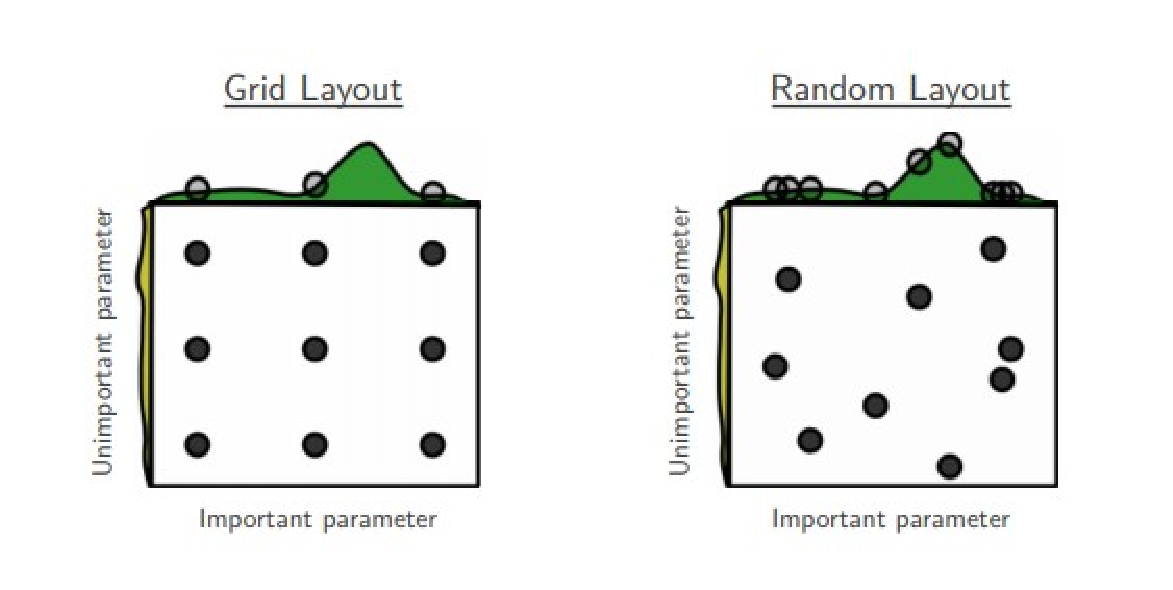
\includegraphics[scale=0.7]{images/chapter_2/random_search.eps}}
\caption{Grid and random search \citep{bergstra2012random}}
\label{fig:Grid and Random Search}
\end{figure}
In Figure \ref{fig:Grid and Random Search} the Grid search and Random search of nine trials are compared for optimising a generic function $f(x, y) = g(x) + h(x)$ where Above each square $g(x)$ is shown in green, and left of each square $h(y)$ is shown in yellow. With grid search, nine trials only test $g(x)$ in three distinct places. With random search, all nine trials explore distinct values of $g$. This failure of grid search is the rule rather than the exception in high dimensional hyper-parameter optimisation.

\subsubsection{Iterative Methods}

In 2011, \citep{bergstra2011algorithms} carried out a state of the art of hyper-parameter optimisation methods for deep neural network models. This work shows the interest of iterative optimisation, based on the criterion of the Expected Improvement of the model performance, proposed by \citep{jones2001taxonomy}. The study introduces two optimisation methods. One method seeks to model the optimisation problem by \textit{Gaussian stochastic processes} (GP) and the second TPE (\textit{Tree-structured Parzen Estimator}) method proposes a kernel-based modelling. These methods are based on the construction of meta-models. The study highlighted the superiority of these two methods over the optimisation by random sampling. In the context of this research work we applied solely the TPE algorithm.

\paragraph{TPE approach} \label{TPE approach}

The Tree-structured Parzen Estimator (TPE) is a sequential model-based optimisation (\textit{SMBO}) approach. SMBO methods sequentially construct models to approximate the performance of hyper-parameters based on historical measurements, and then subsequently choose new hyper-parameters to test based on this model. The TPE approach models $P(x|y)$ and $P(y)$ where x represents hyper-parameters and y the associated quality score. $P(x|y)$ is modelled by transforming the generative process of hyper-parameters, replacing distributions of the configuration prior with non-parametric densities.

In this subsection we have shown how the hyper-parameters can be optimised. Whether it is carried out through a Random sampling approach or through the use of iterative methods, hyper-parameter optimisation is an expensive task in term of computation time. The cost of optimising these models is very high, due to the infinity of possible architectures and the many hyper-parameters, especially for neural networks. In the following subsection, we will present an approach that allows to reduce the overall computational time and which facilitates the convergence of the model, especially if the number of samples composing the training set is not particularly high.


\subsubsection{Transfer Learning} \label{Transfer Learning}

Transfer learning is biologically motivated by the way that humans apply learned knowledge to solve new problems, and consists in exploiting knowledge learned in one problem and searching a good protocol of transferring to a new problem.
In practice, in transfer learning problems, a parametric model is trained in the source problem and transferred to the target problem in a special way, like transferring parameters, or considering the relations between problems. This approach become particularly interesting when we deal with a dataset where the number of samples is small. There is no a well-defined rule to distinguish between a small and a large dataset. Moreover, the amount of data required to solve a machine Learning problem depends on the task that we try to accomplish. In the context of this research project we consider as small, every dataset that have less than 1000 samples. 

Convolutional networks are broadly applicable in the fields mentioned before. The success of transfer learning with convolutional networks relies on the generality of the learned representations that have been constructed from a large database like ImageNet \citep{deng2009imagenet}. \citep{yosinski2014transferable} quantified the transferability of these pieces of information in different layers, e.g. the first layers learn general features, the middle layers learn high-level semantic features and the last layers learn the features that are very specific to a particular task. \citep{zeiler2014visualizing} also visualised the features in the intermediate layers, demonstrating, with images, that convolutional networks learn features from general level to task-specific level. Overall, the learned representations can be conveyed to related but different domains and parameters in the network are reusable for different tasks. The intuition behind transfer learning for image-related tasks is that if a model is trained on a large and general enough dataset, this model will effectively serve as a generic model of the visual world. You can then take advantage of these learned feature maps without having to start from scratch by training a large model on a large dataset.

In practice, we distinguish two successive stages in the training of a neural network by transfer learning: the training of the new last layers, and then the specialisation of the whole network. The first stage is to guarantee the convergence of the classifier on the new task. We seek to obtain a satisfactory inference score. This is why in a first step, only the weights of the neurons of the new last layers are adjusted by back-propagation of the error gradient. Once the convergence of the last layers has been obtained, it is possible to fine-tune the whole network by performing an adjustment of all the weights of the layers in order to improve the classification score.


\section{Conclusion}

In the manufacturing industry, product quality is an indicator for evaluating the production capacity of a company. Customers are increasingly demanding in terms of product quality and providing the customer with a product that complies with the specifications is absolutely essential in a market that is becoming more and more competitive. The best possible solution to deliver 100\% of compliant parts to the customer would be to inspect in details all parts produced. However, most companies cannot test every single product. There may simply be too high a volume or number of them to inspect at a reasonable cost or within a reasonable time frame. Or effective testing might result in the destruction of the product or render it unfit for sale in some way. Moreover, traditional process control approach does not take into account the relationship between process data and produced part quality. In this chapter we have described a general approach that can be applied every time that we want to take advantage of an historical set of data to improve manufactured parts quality. The presented data-driven approach requires 4 main stages: data acquisition, data processing, exploratory data analysis and machine learning modelling. Data acquisition involves the task of identifying all the input process data, as well as the output quality data, that are interesting to try to solve our quality improvement use-case. Data processing is the task of processing and filtering raw input data in order to reduce the noise within data and to make data suitable for Machine Learning modelling. Exploratory data analysis could be used for better understanding the correlation between data and to eventually fine tune the data processing stage. Finally, Machine Learning modelling allows to build a model which relate input process data and output quality data. In such a way it is possible, for a new set of input data, to provide the prediction, or inference of the quality of the finished part. Moreover, using an interpretable model it is possible to identify which process parameters affect the most manufactured parts quality and eventually improve process monitoring. There exists a wide variety of machine learning algorithms. In the second section of this chapter we have presented the linear regression and the linear models with a penalisation term, Tree-Based methods, Support Vector Machines and a few Deep-learning architectures that we have applied all along our research work.

In the following Chapters we will present an application of this method in the industrial context studied along this doctoral studies.


\subsection{Industrial Contribution}

From the industrial point of view, this chapter proposes a new way of looking at process monitoring and quality control. Instead of relying in acceptance sampling method, the historical set of collected data can be leveraged to create an inferring model able to provide a real-time quality inspection without any direct measurement of the part. This would allow for two major benefits:

\begin{itemize}
    \item Faster quality non-conformity detection. In fact, by providing a quality status for each part produced, it is possible to quickly react and adjust the production process to prevent occurrence of new non-conformities.
    \item Destructive tests reduction. If the model is reliable enough to provide accurate results, it is possible to reduce the amount of destructive tests that are regularly performed to assess part quality.
    \item Better comprehension of the production process. If the supervised learning modelling is done through an interpretable Machine Learning algorithm, it is possible to identify which process parameters affect the most part quality. In such a way, it is possible to fine-tune the process by focusing more attention in the control of important parameters. 
\end{itemize}

% Chapter 3
\setcounter{mtc}{5}
\chapter{From corrective to predictive process control} \label{From Corrective to Predictive Process Control}
\minitoc

\section{Introduction}

This chapter describes an application of the previously proposed method to our industrial context. Since out-of-tolerance tank weight is the primary cause of part non-conformity, we investigate process parameters that contribute the most to the variability of tank weight. The first step is to gather a data set representative of the phenomenon to be modelled.  This historical data set is then used to model the relationship between process measurements and part quality. The results, as well as the difficulties encountered when applying such an approach in the industrial context studied will be discussed in detail. Finally, we will show how the results obtained in the framework of this research work have allowed us to identify some areas for improvement in our manufacturing process. 


\section{Motivation}

Poor quality or ``scrap'' parts are very expensive for a company like Plastic Omnium Clean Energy Systems. The “Cost of Non-Quality” (CNQ) is one of the key indicators most used by the company. However, when a part is declared bad, it is first necessary to understand the origin of the problem, which can require a lot of time and energy. Historically, Plastic Omnium industrial process monitoring has been driven using a knowledge-based corrective approach (Figure \ref{fig:Corrective process control}). The quality measurements of each product is used to adjust the process and to maintain the process capability. Moreover, some of the process parameters, which are considered as critic for process safety, are kept under control through the use of uni-variate control charts.  When a parameter falls outside the control limits, some warning messages are generated to alert the operators who have the task of regulating the machine so that the parameter can return in a safe zone. 

\begin{figure}
\centerline{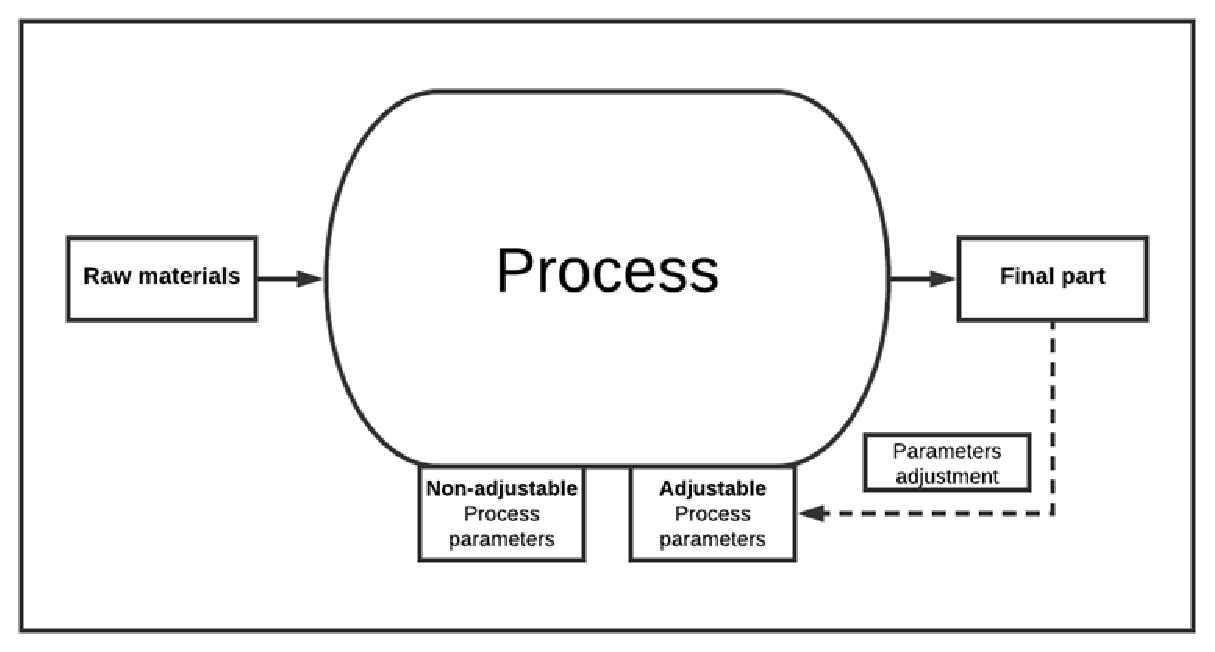
\includegraphics[scale=0.7]{images/chapter_3/corrective_approach.eps}}
\caption{Corrective process control}
\label{fig:Corrective process control}
\end{figure}

Evidence has shown that the overall stability of the process ensures, in most cases, the stability of the product quality. However, it still remains unclear how the system parameters impact the variability of product quality. Quality prediction would allow better adjustment of system parameters at an early stage of production. In other words, anticipation of product quality could be used to adjust the process in real time rather than retrospectively (Figure \ref{fig:Predictive process control}). Such an approach would allow process failures to be anticipated and corrected just-in-time, with an overall reduction in the production of non-conforming parts.

\begin{figure}
\centerline{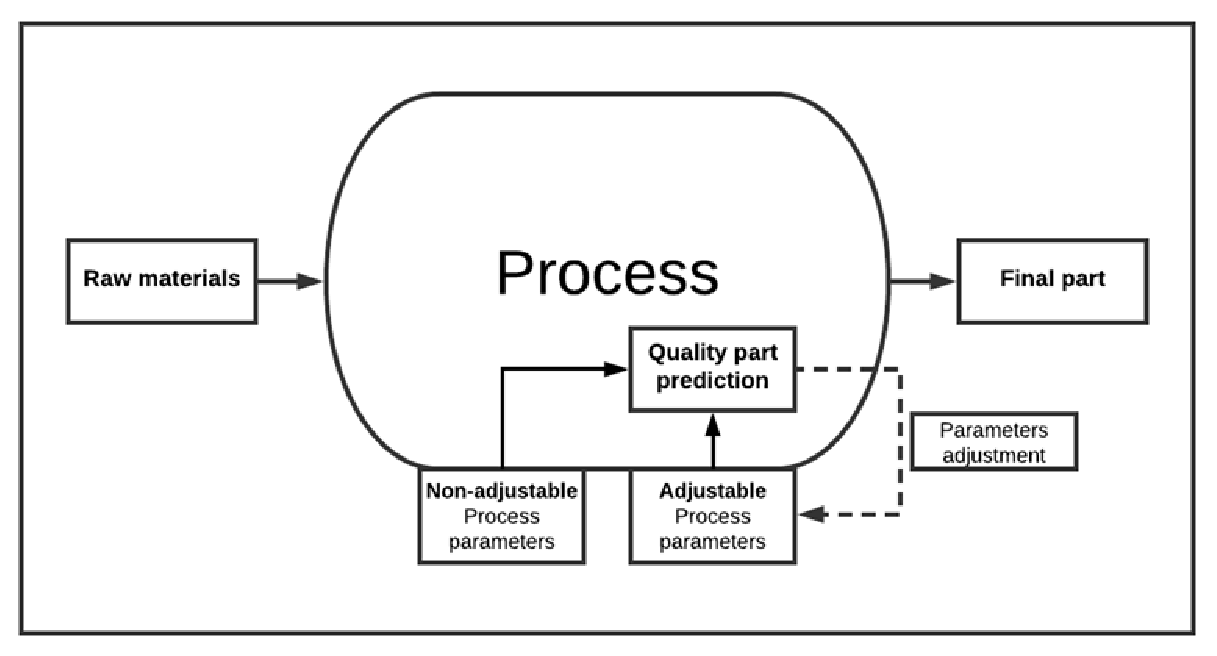
\includegraphics[scale=0.7]{images/chapter_3/predictive_approach.eps}}
\caption{Predictive process control}
\label{fig:Predictive process control}
\end{figure}

In order to understand the correlation between process parameters and the quality of the final part, we use a supervised learning approach. We view our complex industrial process as a black box with multiple inputs and one output. Given $p$ process parameters $(X_1,X_2,\ldots,X_p)$ and one product quality variable $Q$, we look for the function that better approximates the relationship between inputs and the output. Mathematically speaking, we look for the function $f$ that approximates the relationship between the process variables and the quality result:

\begin{equation}
    Y = \hat{f}(X_1,X_2,\ldots,X_p) + \epsilon
    \enspace,
\end{equation}
where $\epsilon$ is defined as the part of $Q$ that cannot be predicted from the input process parameters $(X_1,X_2,\ldots,X_p)$.

By an automatic analysis of a set of examples (training set) of measured input-output behaviour of the process, learning algorithms can find out important correlations between process variables and construct classifiers for detecting dangerous or unwanted process states.

In the context of our research framework, we have carried out a work in order to determinate what are the main causes of scraps involving the extrusion blow-moulding process. An analysis conducted on three years of data collected by the Manufacturing Execution System (MES) software of the company in a French plant has highlighted that the first cause of scraps in blow-moulding machines is due to tanks whose weight does not meet the customer's specifications. This kind of non-compliance accounts for about one half of the total amount of scraps (Figure \ref{fig:Most common scrap causes (2017-2018-2019)}) followed by inclusion and other contamination problems. 

\begin{figure}
\centerline{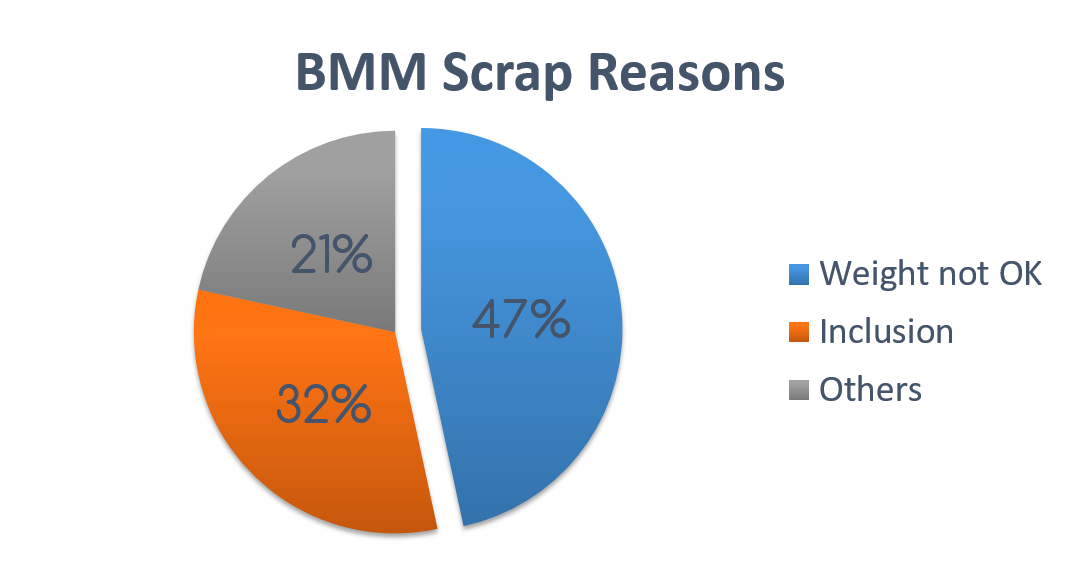
\includegraphics[scale=0.9]{images/chapter_3/Scraps_codes.eps}}
\caption{Most common scrap causes (2017--2019)}
\label{fig:Most common scrap causes (2017-2018-2019)}
\end{figure}

% As presented in Section \ref{The key quality characteristics of a blow-moulded fuel tank}, the tank weight is historically considered as an important product characteristic as it provides an overall indication about the amount of material that composes the fuel tank. By ensuring a lower tolerance limit of the weight it is possible, according to experts, to ensure that there is enough material to ensure compliance of thicknesses. In the same way, there exist an upper tolerance limit which exists to ensure that the part it is not to heavy. By measuring in real-time, for each part produced, the weigh of the tank, people in plants feel reassured about the correct material distribution along its surface.  
As a consequence of this analysis, we decided to focus our efforts on trying to understand where these scraps come from and what we can do to try to reduce them. Moreover, since the weight is measured in real-time, it is possible to easily assemble a dataset composed of multiple samples. By following the approach described in Section \ref{Proposed Method} of this chapters, we aim to search for any hidden pattern or correlation within process data and quality data that could explain why some parts are not compliant in term of weight.


\section{Data collection}

\subsection{Process parameters of the SCADA software}

More than 5000 parameters are measured in real-time at each production cycle of our industrial process. Among these features, some are considered by the experts as critical to ensure the proper stability of the process (see Section \ref{The key parameters of the Extrusion Blow-moulding}). In addition to the critical process parameters there are timer and counter variables. A timer variable accounts for the time needed to execute a particular mechanical movement in the machine production cycle. The sum of all the mechanical times corresponds to the machine cycle time. A counter variable, instead, increases over time because of a particular event. For example, the number of parts produced in a production day is recorded in a counter variable.  

Process parameters are collected by the internally developed SCADA system and data are stored in multiple databases in accordance with the sources of each one. For instance, all the extrusion process data are stored in a database. The same is true for the blow-moulding data and for the weight of the tank that are stored in two separate databases. 

Each process parameter measured in real-time during the production process needs to be associated to the scalar value corresponding to the quality measurement of the manufactured product, at the end of the production cycle. In order to do that, the SCADA software computes some aggregate data to summarise the information in a limited set of scalar features. For each variable belonging to a production cycle, the average, maximum and minimum values are calculated. Then, the SCADA software attaches the aggregates data belonging to a production cycle to a specific traceability serial number which can be used as key to link the different sources of data. 

The extrusion blow-moulding process studied in this work has no system for measuring the parison length. As explained in Section \ref{Industrial domain: extrusion blow-moulding}, the parison length provides information about the material distribution.  Below we present the approach we have used to measure the parison length in real-time.

\subsection{Parison length estimation by computer vision}

The parison length is not available in our process data database because it is not measured. We looked for a measuring system having the following properties:
%
\begin{enumerate}
    \item relatively low software and hardware costs,
    \item requiring little expertise to adapt the model or process the data,
    \item adaptable to changes (for example, adaptable to any blow moulding machine in Plastic Omnium's plants),
    \item making analyses in real time, returning the result with low latency,
    \item able to operate in hostile environments,
    \item be robust to environmental variations (e.g. the system must operate day and night, regardless of lighting conditions).
\end{enumerate}
%
To meet these industrial constraints, we opted for computer vision. Our choice is motivated by the low cost of a camera, its ease of deployment, and the capabilities of deep learning-based models to detect objects in images. In Section \ref{Convolutional Neural Network} we shown how Convolutional Neural Networks reach state-of-the-art results in image classification, object detection and image segmentation tasks. We therefore chose this solution  to detect the parison to measure its length in real time.
The length measurement involves two main stages:
\begin{itemize}
    \item Parison detection: the parison should be detected inside the field of view of the camera. A CNN is trained to detect a (tight) bounding box containing the parison. 
    \item Length measurement: once the parison is detected, its length corresponds to the height of the bounding box.
\end{itemize}

The CNN architecture we chose is \textit{SSD MobileNet-V2}  (see Section \ref{Single Shot MultiBox Detector}), which presents an interesting trade-off between inference speed and model performances in the wild. Here, we expect 
In order to train such a model, 200 images of parisons were collected using a camera of HD resolution ($1280\times720$). By taking images of parisons during extrusion, we built a dataset representative of all possible parison lengths. All images were then annotated using the open source software \textit{Labelme} \citep{wada2016labelme} (Figure \ref{fig:input_and_label}). It is therefore possible to retrieve the bounding box containing the parison.   
\begin{figure}
\centerline{\includegraphics[scale=0.4]{images/chapter_3/input_and_label.png}}
\caption{Input image and parison mask}
\label{fig:input_and_label}
\end{figure}

The data was split into three different subsets: a training set (70\%), a validation set (10\%) and a test set (20\%). The training set samples are used to train the model, the validation set is used during the training to evaluate the performance of the model on unseen samples and to eventually stop the training if the model tends to over-fit. The test set constitutes the subset of samples used to evaluate the performance of the trained model on previously unseen data. The model was trained to minimise the loss function using the  \textit{Adam} optimiser~\citep{kingma2014adam} with the default parameter values ($\beta_{1} = 0.9$, $\beta_{2} = 0.98$ and $\epsilon = 10^{-9}$). The loss function used to train such as model is a combination of a \textit{Localisation loss} and a \textit{Confidence loss}. The localisation loss is the mismatch between the ground truth box and the predicted boundary box. The confidence loss is the loss of making a class prediction. For every positive match prediction, we penalise the loss according to the confidence score of the corresponding class.
% SHOULD I ADD MORE INFORMATION ABOUT THE LOSS ?

To limit the burden of data collection and annotation, we selected only  200 images and we used transfer learning (see Section \ref{Transfer Learning}), with the chosen architecture initialised with the pre-trained coefficients of the \textit{COCO} dataset \citep{lin2014microsoft}. The last linear layer of the model was replaced with a new one matching our problem. Since we are only interested in detecting parisons, the size of our last layer is one.  

SSD MobileNet-V2 provides accurate results in a limited amount of time. Figure \ref{fig:parison_inference} shows two ground truth boundary boxes from the test set and their corresponding prediction. The computation time is below $200$ millisecond on a \textit{Nvidia} Jetson Nano (a small computer equipped with a cheap GPU designed for embedded applications and deep learning based IoT). 
%
\begin{figure}
\centerline{\includegraphics[scale=0.8]{images/chapter_3/parison_length_gt_prediction.png}}
\caption{Two parison length inference examples (from the test set)}
\label{fig:parison_inference}
\end{figure}
%
This system has proven to be robust and to meet the  industrial constraints identified, making accurate and reliable predictions in real time. A simple RGB camera and a small computer offer a cheap, non-intrusive solution that does not require any modification of the machine. 

With regard to our modelling approach we only care about the final parison. The parison length just before the mould closes to blow-mould the final part. We made the assumption that the final length could provide enough information to explain the weight variability.

% INTRODUCE THAT THE CAMERA CAN BE USED TO A BETTER PROCESS CONTROL   

Once the parison length acquisition was running online, we built a dataset with the SCADA software variables and the parison length measurement. We collected data from 5 different batches, corresponding to as many production days, for a total of 5597 samples and more than 5000 features. 

\section{Data processing}

Using all available variables, the number of input features is too large compared to the number of examples in the dataset. We applied two different procedures for variable selection: an expert-based procedure and a statistical-based procedure.

\paragraph{Expertise-based data procedure}

We relied on expert knowledge of the process to discard all features that are not relevant to explain the weight variability. For instance, all counter variables collected by the SCADA software do not bring any interesting information and can be removed. Also, many timer variables, representing the time needed to execute a particular mechanical operation, are redundant and provide no added value. Therefore, most of timer variables have been removed from the dataset.

\paragraph{Statistical-based procedure}

In order to further reduce the number of features, three different statistical feature selection approaches have been used, based on:
\begin{itemize}
    \item correlation between features , 
    \item feature variance,
    \item \textit{stability selection} (see Section \ref{Stability Selection}).
\end{itemize}
%
Removing highly correlated variables eliminates redundant features and reduces collinearity between features that can cause stability problems when fitting the regression model.
%When two or more predictor variables in the same regression model are correlated, they cannot independently predict the value of the dependent variable. In other words, they explain some of the same variance in the dependent variable, which in turn reduces their statistical significance. 
For each pair of features with a correlation value greater than 0.90, one of the two features was removed. Features with very low variance (constant or with no more than 3 different values) were removed. To further reduce the number of features, we applied stability selection. By generating bootstrap samples of the data, and by leveraging the ability of the LASSO penalty to estimate which features are important in each sampled version of the data, we are able to select only those features that have been selected for many perturbed versions of the original problem. Data were finally normalised to have zero-mean and unit-variance (see Section \ref{Data Scaling}). Normalising features is not only important if we are comparing measurements that have different units, but it is also a general requirement for many machine learning algorithms. Figure \ref{fig:data_processing} resumes the data processing flow.
%
\begin{figure}
\centerline{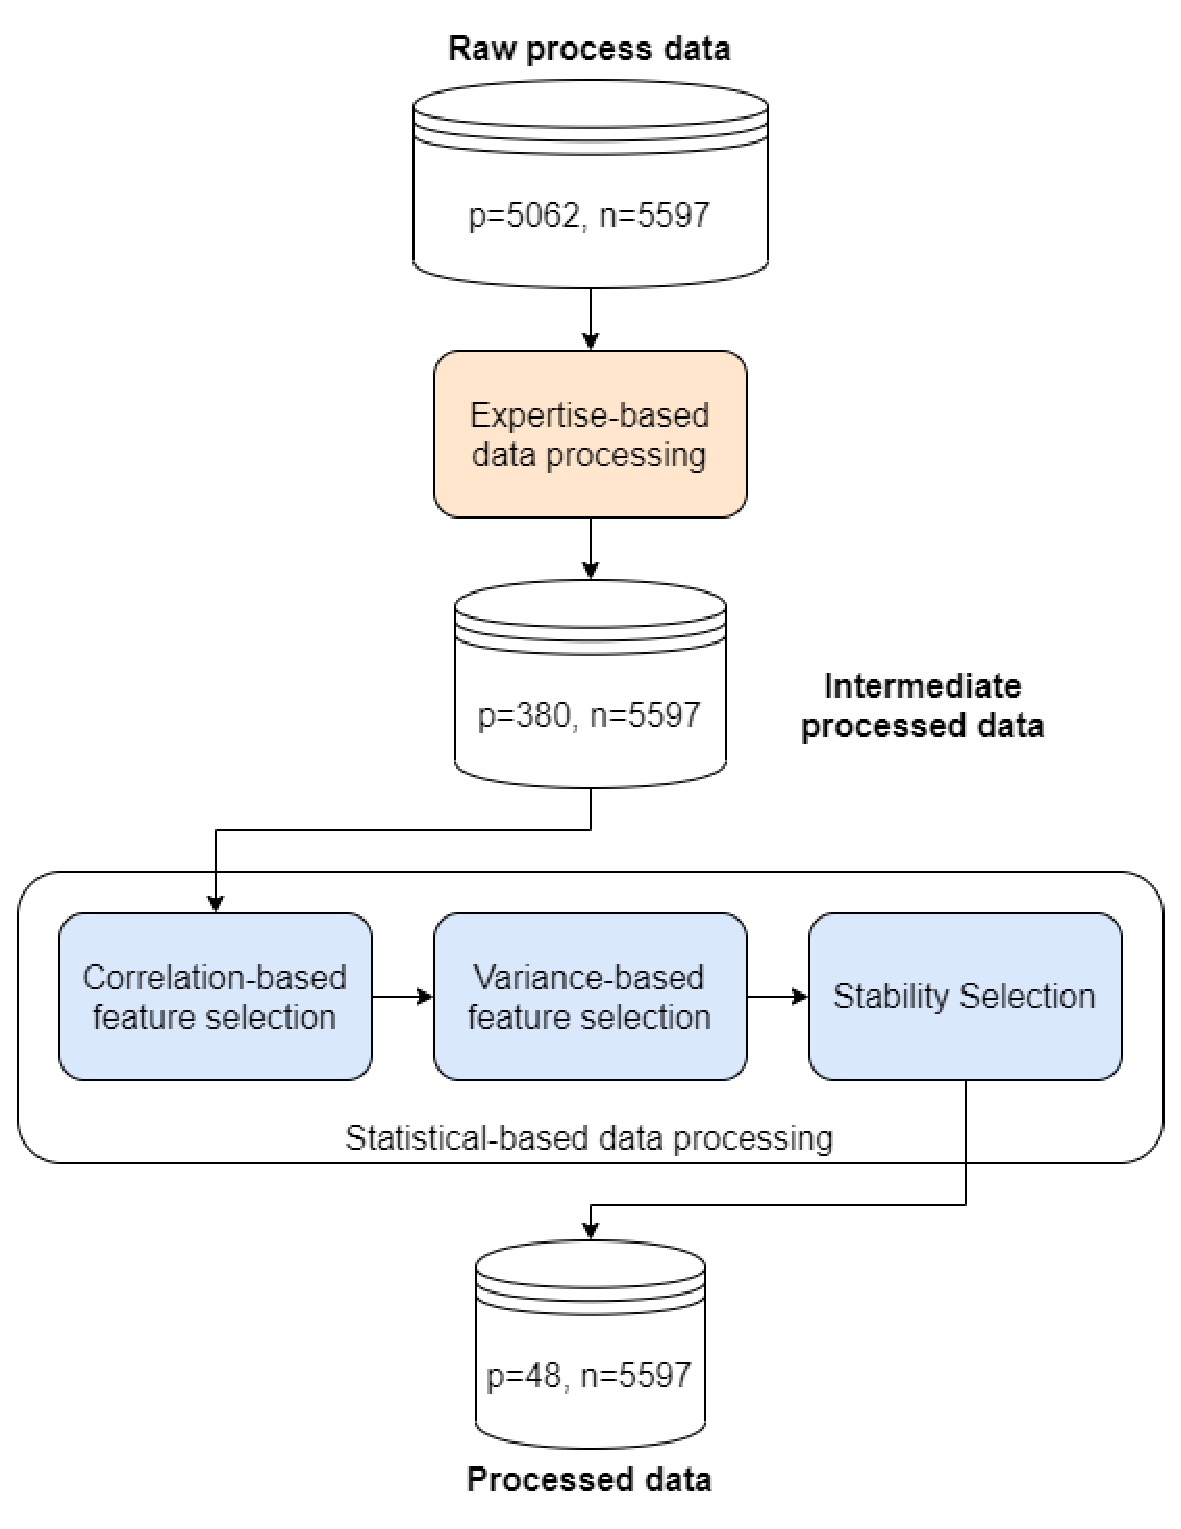
\includegraphics[scale=0.7]{images/chapter_3/Data_processing.eps}}
\caption{Data processing flow}
\label{fig:data_processing}
\end{figure}
%

\section{Exploratory data analysis}

\subsection{Weight versus parison length}

This was the first time that data on parison length was available. The relationship between the parison length just before the blowing phase and the weight of the blown part is illustrated by a scatter plot in Figure \ref{fig:length_weight_scatter}.
%
\begin{figure}
\centerline{\includegraphics[scale=1.2]{images/chapter_3/length_weight_scatter.png}}
\caption{Parison length - Weight scatter plot}
\label{fig:length_weight_scatter}
\end{figure}
%
The plot shows a weak  negative correlation between the parison length and the weight. The Pearson correlation is equal to $-0.32$. The physical explanation is simple: the longer the parison, the less material remains inside the the mould during the blow-moulding. Moreover, the upper part of the parison is often thicker to prevent the parison from breaking under its own weight.  

\subsection{Low dimensional representation} \label{Principal Component Analysis for data exploration}

The large number of features makes it difficult to detect possible hidden patterns in our data by a direct visual representation. We use Principal Component Analysis (see Section \ref{Principal Component Analysis}) to produce the low-dimensional representation that best preserves the distance between examples. 
%
\begin{figure}
\centerline{\includegraphics[scale=0.5]{images/chapter_3/PCA.png}}
\caption{Sample projection on the two first axes of Principal Components Analysis}
\label{fig:pca}
\end{figure}
%
Figure \ref{fig:pca} represents the projection of the samples from 3 batches on the first 2 principal components of PCA. This representation shows two major patterns:
\begin{itemize}
    \item Data are organised in clusters,
    \item For each cluster of data there exist a subset of points moving apart from the cluster.
\end{itemize}
%
Each cluster corresponds to a specific production day or batch. This means that, for the same tank reference, the process parameters differ more between each batch than within a batch. We will call this phenomenon the ``batch effect''. Moreover, the samples are at the periphery of the centre of each cluster correspond to tanks produced in the first two hours after the machine was started. This allows to identify two operating regimes: the \textit{transient} and the \textit{stable} regimes. During the transient regime, the process parameters are slightly different, particularly in terms of temperature. During the transient regime the rate of non-conformity rate in terms of weight is considerably higher (about 300\%) compared to the stable regime.    

\section{Supervised learning modelling}

Given our input processed data $P$ composed of $p$ process parameters and $n$ samples and the output vector $W \in \mathds{R}^{n}$ of the tank the role of the supervised learning modelling is to find the function $\hat{g}$ such that:
%
\begin{equation}
    \hat{g} = \argmin_{g \in \mathcal{G}} \sum_{i=1}^n (W_{i} - g(P_{i}))^{2} \enspace.
\end{equation}
%
We compared several models: ordinary linear regression, Lasso regression, ridge regression (see Section \ref{Parametric models}), random forest and gradient boosting tree (see Section \ref{Tree-based methods}). The choice of these algorithms is motivated by:
%
\begin{itemize}
    \item \textit{Interpretability}: Since we aim to understand which parameters most affect the weight of the blow-moulded tank, we are interested in applying interpretable models. Linear models and tree-based methods are considered to be among the most easily interepretable models.
    \item \textit{Performance}: These methods work quite well with tabular data. When dealing with tabular data, deep learning hardly surpass traditional machine learning algorithms \citep{shwartz2021tabular}. 
\end{itemize}
%
In order to evaluate the predictive power of our models, we used two different approaches: cross-validation and batch cross-validation. 

\paragraph{Cross-validation}

In standard cross-validation, called \textit{K-fold} Cross-validation, the training set is split into $k$ smaller sets. The following procedure is followed for each of the $k$ “folds”:
%
\begin{itemize}
    \item the model is trained using the remaining $k - 1$ folds as the training set,
    \item the error of the resulting model is estimated on the fold set apart from the training set.
\end{itemize}
%
The cross-validation criterion is then the average of error values computed in the loop.
%
\begin{equation}
    CV_{K} = \frac{1}{K}\sum_{i=1}^{K}score_{i}
    \enspace.
\end{equation}
%
This approach is computationally expensive, but does not waste too much data (as is the case when fixing an arbitrary validation set), which is a major advantage in problems where the number of samples is small. In our experiments we used five folds.

\paragraph{Batch cross-validation}

Instead of performing the cross-validation on $k$ random splits of the training set, we split the whole dataset according to the different batches (production days) to cross-validate the model on each batch. Since our dataset comprises 5 different batches, at each time, one batch is used as a validation set and the remaining 4 batches are used to fit the model.

\begin{equation}
    CV_{batch} = \frac{1}{n\degree\;batches}\sum_{i=1}^{n\degree\;batches}score_{i}
    \enspace.
\end{equation}

The mean of the 5 different scores is calculated to have an accurate estimate of the model prediction performance. With this strategy we evaluate whether the models are able to predict on an unseen batch.  


\section{Results and discussion} \label{Results and Discussions}

We use the $R^2$ metric to evaluate the models. Both cross-validation and batch cross-validation return negative $R^2$ values for all the models. 
This means that the models are worse at predicting the weight than the sample mean, and thus that the variability of the weight cannot be explained by the available parameters of the process. Results for cross-validation are resumed in Table \ref{tab:cross_validation_results}.  

\begin{table}[]
\centering
\caption{Cross-Validation results}
\label{tab:cross_validation_results}
\begin{tabular}{lllll}
\toprule
\textbf{Algorithm} & \textbf{R² train} & \textbf{R² test} \\
\midrule
Linear regression   & 0.72   & -0.34    \\ 
Lasso regression    & 0.80   & -0.25    \\ 
Ridge regression    & 0.78   & -0.26    \\ 
Random forest       & 0.94   & 0.05     \\ 
Gradient boosting   & 0.95   & -0.11    \\ 
\bottomrule
\end{tabular}
\end{table}


\begin{table}[]
\centering
\caption{Batch cross-validation results}
\label{tab:batch_cross_validation_results}
\begin{tabular}{lllll}
\toprule
\textbf{Algorithm} & \textbf{R² train} & \textbf{R² test} \\
\midrule
Linear regression    & 0.50   & -1.34  \\ 
Lasso regression     & 0.62   & -0.45  \\ 
Ridge regression     & 0.67   & -0.39  \\ 
Random forest        & 0.81   & -0.27  \\ 
Gradient boosting    & 0.76   & -0.73  \\ 
\bottomrule
\end{tabular}
\end{table}

Both tables highlight how all the approaches tend to over-fit but struggle in generalise what has been learned on the train set to unseen new samples. This is especially true for tree-based methods that in general are more prone to over-fit. 

Results are quite astonishing but are showing evidence that it could be hard to apply statistical models in a field, manufacturing industry, where there is a lot of uncertainty. A further analysis was conducted to try to explain and motivate these results. We have identified six possibles reasons for these negative results:
%
\begin{enumerate}
    \item \textit{Non-stationarity of data}
    \item \textit{Lack of data characterising the properties of the raw material}
    \item \textit{Low variability in product quality}
    \item \textit{Reliability of the input data}
    \item \textit{Weight too resultant}
\end{enumerate}
%
The following paragraphs provide more detail about each  source of error identified. 

\paragraph{Non-stationarity of data}

Results obtained with batch cross-validation show that our models do not generalise among different batches. Actually if we look at distributions of our input features we can see how they change considerably among different batches (Figure \ref{fig:Example of a process parameter variability in probability distribution}). 
%
\begin{figure}
\centerline{\includegraphics[scale=0.4]{images/chapter_3/process_parameter.eps}}
\caption{Probability distributions across batches for a particular process parameter}
\label{fig:Example of a process parameter variability in probability distribution}
\end{figure}
%
A “Two-sample Kolmogorov-Smirnov” test was applied to all pairs of batches. According to these tests, only 35\% of the input features share the same probability distribution over all batches (at a $0.95$ confidence level).
Standard machine learning models rely on stationarity hypothesis to generalise: a trained model expects that the test distribution follows the distribution of data used to train the model.

\paragraph{Lack of data characterising raw material properties}

The change in data distribution may also be due to some external events or factors that we do not control and do not take into account within our own input process data. We claim that the ``batch effect'' we observe in the data could be a consequence of certain changes in the rheological properties of raw materials. In fact, the final part is the result of the transformation of raw material through our complex process. Unfortunately, to this date, these data are not available and they cannot be integrated in our dataset. Further studies have been carried out in order to see if it is possible to measure some rheological properties of the material in real-time. There are industrial on-line rheological systems that provide continuous measurements of the melt flow rate or apparent viscosity directly on the manufacturing process. Unfortunately, this solution is not economically viable, especially as such a system would have to be installed for each of the 6 screws.

\paragraph{Low variability in product quality}

The manufacturing process is already relatively reliable and stable, with low variability in product quality. The scrap rate is under 3\% and the tolerance limits set to evaluate the compliance of blow-moulded tanks are quite strict. In general, a weight variability of about 300 grams is sought, which for an average tank weight of $8.5$ kilograms corresponds to about $3.5\%$ of the total weight. The phenomenon modelled would have been more pronounced, and the problem would have been simpler with a larger weight variation.     

\paragraph{Reliability of the input data}

As we look for small variations of weight, it is important that the input data is accurate enough. In an industrial environment, such as a production plant, the collected data are most of the time noisy. The maintenance of the sensors cannot be done regularly. As a consequence, some sensors may provide erroneous values. Moreover, the SCADA software computes some aggregate operation on the input time series-data, which can lead to a loss of information. Finally, it is quite complex to attach extrusion data to the traceability serial number of a tank since extrusion is a continuous process and there are no precise triggers to define what data belongs to a given part. The extrusion data may be misaligned with the manufactured part.  

\paragraph{Weight too resultant}

Another possible explanation is directly related to the nature of the output variable considered in our problem, the weight. In fact, the weight is a resulting variable which depends on the distribution of the material on the tank surface. However, different material distributions can produce the same final weight. In others words, different manufacturing conditions, represented by different process parameters values can lead to the same weight. As a consequence, the model struggles to learn the function which approximates the relationship between process parameters and quality data.

These results highlights the difficulties we can encounter when dealing with manufacturing process data. However, in the following section we will show how the work presented in this chapter has made it possible to start a new project to improve the manufacturing process. 


\section{SmartBMM: towards smarter machines}

The data analysis results presented all along this chapter have shown the inability to explain the tank weight variability given the blow-moulding process data that are considered as critical by process experts. The possible reasons have been discussed in detail in the previous section. What the analysis has also highlighted is that the most scrap occurs just after the machine start-ups (see Section \ref{Principal Component Analysis for data exploration}). As shown previously, right after the machine start-up, the extrusion blow-moulding process is not completely stable which increases the overall scrap rate of the blow-moulded parts. Moreover, an interview of different extrusion blow-moulding experts has highlighted that there are no common and shared best practices to start the machine. As a consequence,  there is a lot of variability between startups.

\begin{figure}
\centerline{\includegraphics[scale=0.7]{images/chapter_3/smartbmm_barchart.png}}
\caption{Time and scrap rate variability for 27 machine start-ups in a Plastic Omnium plant}
\label{fig:smartbmm_barchart}
\end{figure}
%
Figure \ref{fig:smartbmm_barchart} illustrates this variability among 27 machine start-ups performed in a Plastic Omnium plant. On the left bar-chart, we can see how the time needed to start the machine changes from a start-up to another. Sometimes the start-up is done in 10 minutes, other times a full one may take around 15-20 minutes. There are also three occurrences for which the start-up took more than 20 minutes. The right bar-chart reports the scrap rate in the first 60 minutes. Most of the time, the scrap rate does not exceed 5\%, but there are some starting for which the scrap rate is above 10\%. These observations call for some efforts to improve the way the extrusion of blow-moulded machines is started. By automating and by optimising the machine start-up we should reduce the uncertainty introduced by manual starts. This would allow for a faster convergence towards the stable regime of the machine and, as a consequence, to a smaller number of part non-conformities.   

%We are aware that the scraps may have a multitude of reasons which do not depend on the way the machine is started, but we claim that providing repeatable and optimised starting should benefit at the overall performance of the manufacturing process. 
The project was initially conceived to handle just the machine starting phase but later on, it was extended to also cover the purge cycles of the machine. Indeed, ensuring good purge cycles reduces the risk of contamination/inclusion problems. In this context, we have developed the \textit{SmartBMM} solution. \textit{SmartBMM} is a software which leverages the real-time data collected directly from the PLC of the machine and the past data to follow the best instructions to get the machine started without any manual intervention of the operators.

\begin{figure}
\centerline{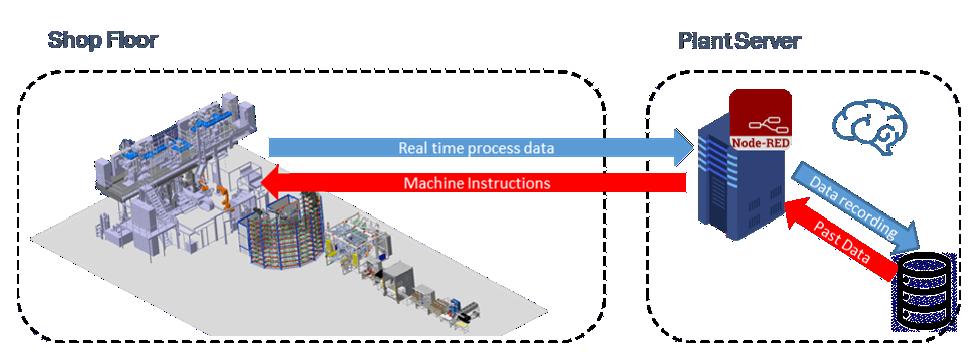
\includegraphics[scale=1]{images/chapter_3/SmartBMM.eps}}
\caption{\textit{SmartBMM} software}
\label{fig:SmartBMM}
\end{figure}

Figure \ref{fig:SmartBMM} shows broadly how the SmartBMM works. The SmartBMM software collects real time data directly from the PLC and stores it in a database for later retrieval. When the SmartBMM software is started the data collection continues, but, this time, the machine starts to write information to the PLC to execute a set of operations. The software takes the real time incoming data and the past data to elaborate the machine instructions to bring the machine to production conditions. The stored data are used to compute production extruder speeds which, accordingly to past data, minimise the non-conformity rate. Looking at previous production runs we are able to retrieve the process conditions which lead to a better performance and a lower scrap rate. The software is developed using the \textit{Node-RED} \citep{nodered} programming tool. Node-red is a low-code programming for event-driven applications which was specifically designed to work with IoT and that allows easy interfacing with machines through different communication protocols.

Instead of manually start the machine by pressing simultaneously multiple buttons on the HMI (Human Machine Interface), machine setters and operators have to press only one button to start a cycle, whether it is a \textit{starting} cycle or a \textit{purge} cycle.  

\begin{itemize}
    \item The starting functionalities leverages the real-time data collected directly from the PLC of the machine and the past data to elaborate the best instructions to get the machine started without any manual intervention of machine operators. The set of consecutive instructions provided to the machine are fairly standard. The extruders are started, then the material is fed into the screw, then the extruder speed is raised and so on. However, our system does not rely on timers to trigger the machine instructions. In real time the process status is controlled and the next machine instruction is triggered only if the process meets all requirements.
    Two starting functionalities are available: \textit{full} and \textit{downtime}. The first one executes a starting phase when the machine is completely stopped; the second one returns to the production condition in which the machine was temporarily idled.
    %  There exist two Purge cycles: the \textit{Purge Out} and the \textit{Purge In}. The Purge Out cycle is done when the machine is stopped for more than 2 hours to remove any FINIRE. The Purge In is done every time that the Purge Out has been done to prepare the extruder for the production run. 
    \item The purge functionalities allow to improve purge cycles of the machine.
    During purge cycles we want to ensure that enough material transits into the extruders at high pressure to clean them of residual production material. Instead of relying on fixed speed values or timers, we have developed a \textit{PID controller} that regulates the extruder speeds to ensure that they are constantly above the pressure targets. Moreover, the amount of material transiting through the screws is controlled in real-time. This allows to finish the purge cycle only when the correct amount of material has transited through the screws.     
\end{itemize}
%
The starting and purge functionalities reduce the ``weight not OK'' and the ``contamination'' scraps, which account for $2/3$ of the total amount of non-conformities.
The functionality is chosen by the operator through a graphical user interface (GUI) specifically developed to allow an easy interaction with the software (Figure \ref{fig:SmartBMM_gui}).
%
\begin{figure}
\centerline{\includegraphics[scale=0.5]{images/chapter_3/SmartBMM_gui.png}}
\caption{\textit{SmartBMM} GUI}
\label{fig:SmartBMM_gui}
\end{figure}
%
Historically, all manufacturing processes, including extrusion  blow-moulding, rely on PLC programs to execute the set of instructions to allow the manufacturing machine to work correctly and to allow for the transformation of raw materials into finished products. In this project, we decided to pilot the machine outside of the machine PLC for the following reasons:
%
\begin{itemize}
    \item PLCs are very robust and safe, but they lack flexibility. PLCs are conceived to execute a set of logical instructions but they do not lend themselves well to be used concurrently with other systems such as databases. Developing a more complex logic which involves data storage and communication with databases is by far more easy with traditional software development tools.
    \item Implementing the logic on an external system such as a physical or a virtual server reduces the number of PLC modifications of the machine. Our software is  non-intrusive and can be installed remotely on a server without any direct modification of the PLC program. It is something that can be plugged to the machine to introduce new functionalities. This reduces costs considerably, since it does not require the intervention of an external consultant.
\end{itemize}
%
This strategy has, however, a main drawback. Our tools completely rely on plant network to communicate instructions to the PLC. Which means that a bad network could be a bottleneck for the correct functioning of our software. Security features have been added on the software side to interrupt the communication with the machine if any network failures prevents to communicate with the machine.
In our opinion this is an example of a cyber-physical system. SmartBMM leverages the sensor networks with data processing to monitor and control physical environment, with feedback loops able to elaborate the best set of machine instructions given the different process conditions.


\section{Conclusion}

In this chapter, we have presented an empirical evaluation of our approach in the industrial context. The features currently collected by home made \textit{SCADA system}, even when enriched by parison length measurements, cannot predict the tank weights. These results show the difficulty of applying statistical models in batch manufacturing industries, where it is not always possible to have knowledge of all the elements that contribute to the variability of the part quality. Possible explanations for these results were discussed. Nevertheless, this research work has allowed the identification of avenues for improvement of the blow-moulding process. In particular, the exploratory data analysis has shown how most of the part non-conformities occur just after machine start-up, when the process is not yet stable. This led to the launch the \textit{SmartBMM} project.

\subsection{Scientific Contribution}

The results presented in this chapter question the effectiveness of data-driven methods in certain manufacturing contexts. The end-to-end data-driven methods have proven to be effective in many applications, but for them to work well, informative data on a stationary phenomenon is required. In other situations, it may be better to decompose the original problem into several sub-problems with properly controlled data quality. The following chapter will present such an approach.

\subsection{Industrial Contribution}

This chapter presents three main industrial contributions.
\begin{itemize}
    \item Firstly, the work challenges certain beliefs about the operation of the blow-moulding process. The process parameters considered critical to ensure proper functioning of the process do not explain the variability in tank weights. The control limits previously set for the critical parameters of the process to ensure the correct functioning of the production process were found to be insufficient for providing such an explanation.
    \item The parison length measurement has opened new research perspectives. By measuring in real-time the length of the parison, we will eventually be able to control the distribution of material over the entire length of the parison to improve the quality of the manufactured parts. Further information and perspectives will be presented in Chapter \ref{Contributions and perspectives}.
    \item Finally, the \textit{SmartBMM} software that was developed starting from the results obtained trough the data analysis process has been used to improve the machine start-up phases which lead to a high scrap rate. By ensuring a better start-up, we reduce the transient phase and thus the percentage of parts that do not meet quality standards. Future works will make use of the parison length measured by the camera to add to SmartBMM new functionalities.  
\end{itemize}



% Chapter 4
\setcounter{mtc}{6}
\chapter{Towards model-based quality control}
\minitoc

% A few considerations:
% 1) The mathematical notation should be changed accordingly to Yves's suggestion in the paper
% 2) Some Figure could be replaced or improved. For instance, the Figure 4.7 should be replaced as well as the 4.15.


\section{Introduction}


In the manufacturing industry, product quality is an indicator for evaluating the production capacity of a company. Customers are increasingly demanding in terms of product quality and providing the customer with a product that complies with the specifications is absolutely essential in a market that is becoming more and more competitive. The best possible solution to deliver 100\% of compliant parts to the customer would be to inspect in details all parts produced. However, most companies cannot test every single product. There may simply be too high a volume or number of them to inspect at a reasonable cost or within a reasonable time frame. Or effective testing might result in the destruction of the product or render it unfit for sale in some way. Traditional quality inspection technology is the result of single variable statistical process control and sampling inspection.

One set of statistical tools for applying such a screening is acceptance sampling. Using such tools enables decision makers to determine what action to take on a batch of products. Decisions based on frequency testing, rather than on 100\% inspection, are more expedient and cost effective but it cannot guarantee the conformity of all parts of the population from which the sample was drawn~\citep{fuchs1998multivariate}.

In this chapter, we propose a new approach to perform a real-time, non-destructive quality control to measure thicknesses of blow-molded parts. The proposed approach makes use of deep learning data-driven methods to leverage the thermal inertia of the manufactured plastic part, captured through the use of thermal imaging, to infer the thicknesses of the part surface without any direct measurement. Compared to traditional quality inspection approaches, which aim to detect visual defects of manufactured products, our approach leverages thermal information to perform a non-visual quality control. 
%
The first experimental results on real industrial data are very promising and demonstrate that the proposed methods could achieve satisfactory performance for industrial usage.

\section{Towards data-driven quality control}

In this section, we extend the concept that was presented in Chapter \ref{From Corrective to Predictive Process Control} in order to develop a general framework for inferring the quality of a manufactured part without directly measuring it. One more time, we will take advantage of the ability of machine learning to learn the transfer function from some input data to the product quality. The trained model could then be applied to enhance the manufacturing quality control by providing a quality status to the part.

Historically, in the manufacturing industry, and in particular in the research framework that have been studied during this PhD study, the real quality control is a time-consuming operation that requires several minutes of work and that cannot be done online for each part. As a consequence, the only method that fits these production constraints is the \textit{Acceptance sampling} method. One part per \textit{X} parts produced is physically measured and the quality of the entire production batch is determined by the result obtained from the measurement on the individual sample. Figure \ref{fig:statistical_quality_control} outlines the functioning of acceptance sampling. 

\begin{figure}
\centering
\includegraphics[scale=0.50]{images/chapter_4/statistical_quality_control.png}
\caption{Statistical quality control}
\label{fig:statistical_quality_control}
\end{figure}

Although this method is widely applied in the manufacturing industry and it is globally accepted, it presents two major drawbacks:
\begin{enumerate}
    \item The acceptance sampling method is able to track deviations in product quality, but it is not able to provide 100\% quality inspection. As a result, it may happen that one or multiples non-compliant parts are produced, as a response to a temporary malfunction in the production process, and these parts may not be detected. This may result in one or multiple non-compliant parts being sent to the customer.
    \item The second drawback of Acceptance Sampling is the delay in detecting a process deviation. If product quality starts to deviate, the manufacturer has to wait for the next quality control to identify the problem and to be able to act on the process to correct it. Moreover, the parts produced in this time frame are potentially non-compliant and extra time-consuming quality control may be required to establish whether or not the parts can be sent to the customer.
\end{enumerate}

Another problem to consider, is the one related to the destruction of the pieces being measured. In fact, some quality measurements involve the destruction of the part or some modifications that make it unsuitable for sale to the customer. For instance, advanced quality control for assessing the material distribution of each thickness layer of a blow-molded part requires the cutting of the piece in small samples, subsequently analyzed in the laboratory. Even if these tests are necessary and important to certify the conformity of the part, it constitutes a source of waste for the manufacturer, increasing the number of PPM (parts per million) defects. 

In order to improve the quality control of the parts, we propose to perform a comprehensive quality control using a machine learning based approach. The idea is to infer the quality status of each part produced through the use of a machine learning algorithm. Unlike in Chapter 3, we are not bound to use the process data as a predictor for our model, because we are only interested in providing a status to a manufactured part and we are not directly concerned by the production process. New sensors or cameras may be installed to recover new sources of data ``close'' to the final product.

In the context of this PhD study, the approach of inferring the quality of a part using a trained machine learning algorithm is called \textit{data driven model-based quality control}.
The benefits that this approach can bring to quality control throughout the manufacturing industry are manifold. First, it ensures a 100\% quality control on all parts produced which enable for a fast reaction to quality non-conformities (Figure \ref{fig:model_quality_control} on the left side). In fact, by ``virtually'' measuring each part, we are able to eventually discard parts for which the model has provided a ``Not-OK'' result, or request the quality team to carry out more in-depth tests. Model-based quality measurement may be effectively used to detect those parts that turn out to be, from a statistical point of view, outliers. In this way, instead of randomly sampling the parts to be measured by the quality operators, the model is able to suggest the parts that seem to be interesting.
By discarding all non-compliant parts, this approach indirectly reduces product recalls and thus the whole series of requests to return, exchange or replace a product that has been found to be defective, and which could impair performance, harm consumers or cause legal problems for producers.

\begin{landscape}
\begin{figure}
\centering
\includegraphics[scale=0.50]{images/chapter_4/data_driven_model.png}
\caption{Data-driven model-based quality control}
\label{fig:model_quality_control}
\end{figure}
\end{landscape}

If the trained model is sufficiently robust and accurate at predicting the quality status of a part, a second stage would be to reduce the real quality controls which destroy the parts or makes them unusable (Figure \ref{fig:model_quality_control} on the right side). In such a case, not only the model-based control would be able to provide a thorough quality control, but it would also be able to reduce the quality PPM which account for an overall better production performance. Of course, real part measurements cannot be completely replaced by model-based measurements. In fact, real measurements are the primary data source for training the data-driven model. 

\section{Thickness inference using thermal imaging}

\subsection{Context and background} \label{Context and background}

In Blow-molded parts the material distribution all over the part surface plays a key role in ensuring that the finished product meets customer specifications. The thickness of the tank over the whole surface must be enough to ensure the robustness of the part and therefore its safety, while avoiding an excessive and unnecessary weight of the finished product. Measuring the thickness of a blow-molded part over its entire surface is trivial because most of the blow-molded parts are hollow, which limits how the thickness can be measured. Traditional methods to measure the thickness of hollow parts involve the use of ultrasonic measuring instruments that provide satisfactory results while avoiding the destruction of parts. The main idea of \textit{Ultrasonic Thickness Measurement} (UTM) is to measure the time needed for the ultrasonic wave to traverse the material. Some of the advantages of UTM over other nondestructive methods are:
\begin{itemize}
    \item the possibility to measure parts with just one accessible surface,
    \item no need for laboratory conditions,
    \item  its high sensitivity and accuracy.
\end{itemize}
 
Although these methods are extremely high-performance for sample quality control, they present a major drawback: they cannot be used for online measurement. The measurement of a large number of points, which is necessary to estimate the distribution of the material over the entire surface, is time-consuming and cannot be applied online in production. Hence, the quality control of the thickness can only be carried using a sampling approach. Recently, new technologies involving the use of terahertz waves have been developed to accurately measure the thickness of materials without any contact with the material itself. These methods have proven to be extremely powerful for measuring the thickness of automobile paint \citep{su2014terahertz,krimi2016highly}, or pharmaceutical tablets \citep{may2011terahertz}. Of all the methods found in the literature, terahertz-based systems seem to be the only ones that can be used to perform real-time thickness measurement, but in order to use it in real-time, the measurement sensor must be installed on a robot, or collaborative robot, which can significantly affect the price of the complete measurement solution.

Another well-known technique for measuring thickness of parts is \textit{Computed Tomography} (CT). Typical areas of use for CT in industry are in the detection of flaws such as voids and cracks, and particle analysis in materials. In metrology, CT allows measurements of the external as well as the internal geometry of complex parts. As stated by \citet{de2014industrial}, CT is particularly suitable to investigate molded polymer parts, thanks to the good penetrability of X-rays in these materials. Even if CT-based techniques are extremely powerful, they require laboratory conditions and  do not lend themselves well to real-time thickness control. Moreover, this equipment may be very expensive, questioning its profitability.
%
Eddy current testing, widely applied for the non-destructive thickness measurement of metallic parts \citep{cheng2017thickness,mao2016thickness,wang2015noncontact,yin2007thickness}  is also non-destructive, but cannot be used as polymers composing the blow-molded part are not conductive.

\textit{Thermal Imaging}, a non-contact technology capable of measuring large surfaces in a single shot, has been applied to different kinds of thickness prediction methods in the last decades \citep{sun2003method,sun2006analysis,choi2008quantitative,benitez2008definition,zeng2012absolute,li2018thickness,he2013eddy}. Among the most widely used thermal imaging approaches we can mention: \textit{Pulsed thermography} in which a brief controlled thermal stimulation pulse is applied on the tested piece, \textit{Step heating thermography} in which a continuous, uniform heat flow is applied for a long period, and \textit{Lockin thermography} in which a periodic heat input is used. The main idea behind all these approaches is to transfer energy to the test piece and to monitor its surface temperature evolution over time. In flash thermal imaging, for example, some flash lamps provide the thermal impulse, and the infrared camera monitors the surface-temperature decay on the heated surface. On the other hand, step-heating thermal imaging is using a long pulse of low intensity heat stimulation. Unlike pulsed thermal imaging, step-heating technology monitors the temperature raise over time while the heat energy is transferred to the test piece.
The approach of monitoring the surface-temperature may also be applied without actively providing heat to the test part, especially for parts that are still hot after the manufacturing process. This is definitely the case of blow-molded parts. Even if the part surface is cooled inside the molds during the blowing process, thicker blow-molded products still have high temperatures and it takes several minutes for the work-piece to reach the temperature of the environment in which it is cooled.

\subsection{Motivation} \label{Motivation}

Our work is motivated by the empirical observation of the cooling of blow-molded parts in the first minutes after blowing. Areas of the parts have different cooling behaviours depending on their thickness. 

Areas with smaller thicknesses cool down faster than those with larger thicknesses. For the thicker zones, the surface temperature even starts to increase before decreasing (Figure~\ref{fig:temperature_cooling}).
%
\begin{figure}
\centering
\includegraphics[scale=0.55]{images/chapter_4/cooling.eps}
\caption{Surface temperature cooling profiles at the thinnest (left) and thickest (right) areas of the blow-molded part}
\label{fig:temperature_cooling}
\end{figure}
%
This phenomenon is due to the release of energy from the innermost plastic layer that has not be in direct contact with the mold surfaces.
As suggested by the literature presented in Section \ref{Context and background}, this surface temperature decay, easily measured by thermal imaging, could be leveraged to infer the thickness of the part.  
In particular, we make two assumptions:
\begin{itemize}
   \item The cooling conditions of the environment where the part is monitored are the same for all parts produced. Therefore, we consider that the variations of the temperature of the production area are negligible.
   \item The physical and chemical properties of the material are assumed to be constant over the entire surface of the part. In particular, the thermal and infrared transmittances of the material should be approximately constant.
\end{itemize}

Based on these assumptions, we designed two data-driven methods to model the relationship between the surface temperature variations of critical areas of the part and the corresponding thickness values. The first approach, by one-dimensional time series, exploits the cooling dynamics, one point of the part at a time, whereas the second method processes the part globally, taking into account unity of part (points belonging to the same part are processed simultaneously) and spatial information (points are positioned on the part surface).

\subsection{Proposed methods}

In this section, we present new approaches to predict the thickness of blow-molded parts. We propose a non-intrusive real-time thickness inference exploiting the variations of surface temperatures over time on different areas of the blow-molded part. 
Unlike traditional thickness quality control methods, our system is able to predict thickness values at critical points of the part within minutes, allowing real-time operation.

Three different approaches to model the temperature-thickness relationship are proposed:
%
\begin{itemize}
    \item \textit{Functional approach}: The Functional approach involves the use of a parametric function to approximate the pixel-wise temperature surface decay. The function parameters, retrieved through the use of a curve fitting approach, may then be used as input features for a machine learning regressor.
    \item \textit{Temporal approach}: The Temporal approach, as the Functional one, takes advantage of the pixel-wise temperature decay. Instead of compressing the information through the use of a parametric function, the temporal approach leverages the ability of deep learning to extract meaningful features from raw signals.
    \item \textit{Spatial-Temporal approach}: The Spatial-Temporal approach leverages not only the temporal temperature information, but also the spatial one. Instead of extracting the temperature time series for each critical point of the blow-molded parts we can design an \textit{end-to-end} deep learning architecture able to directly handle the input thermal video. In such a way, we should be able to take into consideration not only the surface-temperature evolution of a point but also its position on the spatial dimension. 
\end{itemize}
%
These three approaches are presented in more detail below.

\subsubsection{Functional approach} \label{Functional approach}

The first approach consists of three phases: time series extraction, time series approximation by parametric curve fitting and thickness prediction using the parameters of the approximated temperature surface decay.

\paragraph{Time series extraction:} 

The time series extraction phase aims to process the input thermal video in order to retrieve the temperature time series of a limited number of critical points, for which the thickness value is known. These time series constitute the input data of our data-driven model.
Given $n$ critical points of each part, for which the thickness values are known, and given its thermal video $X^i$, we are interested in extracting the time series $ts^{i}_{(x_j, y_j)}$ where $j \in [1,n]$. For a set of $m$ input thermal video, this first phase produce a dataset
\begin{equation}
    D = \{(ts^{i}_{(x_j, y_j)}, y^{i}_{(x_j, y_j)});i \in [1, m]; j \in [1, n]\},
\end{equation}
composed of $n\times m$ collection pairs $(ts^{i}_{(x_j, y_j)}, y^{i}_{(x_j, y_j)})$ where $ts^{i}_{(x_j, y_j)}$ is the $j$-th time series extracted from the thermal video $i$ and $y^{i}_{(x_j, y_j)}$ is the corresponding thickness value. 

\paragraph{Time series approximation:}

In order to reduce the number of input features we made to choice to approximate the surface-temperature decay time series through the use of parametric function. Approximating the time series with a parametric function would allow to compress the temporal information in a limited number of new features, corresponding to the parameters of the function. Temperature-surface time series have a fairly simple shape to approximate (Figure \ref{fig:temperature_cooling}). The predominantly parabolic shape of the time series lends itself well to be approximated with a quite simple function with a few parameters. We compared the following three parametric models in order to find the one that best fits our time series:
\begin{itemize}
    \item Power Law: $y=ax^b$
    \item Polynomial (2° degree): $y=ax^2+bx+c$
    \item Logarithmic: $y=a+b\log(x)$
\end{itemize}

In such a way, the different cooling behaviour, observable in different areas of the part could be expressed through a limited number of new parameters (Figure \ref{fig:parametric_approximation}. Moreover, the functional approximation smooths the time signal, thereby reducing the measurement noise. The new features may be then used as the input data for a regression model. Mathematically speaking, the time series approximation produces a new dataset,
%
\begin{equation*}
    D = \{(z^{i}_{(x_j, y_j)}, y^{i}_{(x_j, y_j)});i \in [1, m]; j \in [1, n]\}
    \enspace,
\end{equation*}
%
composed of $n\times m$ collection pairs $(z^{i}_{(x_j, y_j)}, y^{i}_{(x_j, y_j)})$ where $z^{i}_{(x_j, y_j)}$ is the $j$-th set of parameters obtained by fitting the parametric function. 

\begin{figure}
\centering
\includegraphics[scale=0.9]{images/chapter_4/Parametric approximation (Polynomial).png}
\caption{Parametric approximation}
\label{fig:parametric_approximation}
\end{figure}

\paragraph{Time series regression:}
Parametric models such as \textit{Lasso Regression} (\ref{Parametric models}), or Decision-Tree based methods such as \textit{random forest} (\ref{Tree-based methods}) or even \textit{Support Vector Machine} (\ref{Support Vector Machines}) methods may than be applied to try to predict the thickness value of a given area based on the parametric features computed through the functional fitting of the surface-temperature time series. The role of the machine learning model is to learn the transfer function $\hat{f}$ which satisfies the following equation:

\begin{equation}
    y^{i}_{(x_j,y_j)} = \hat{f}(z^{i}_{(x_j, y_j)}; i \in \{1, \ldots,n\}; j \in \{1, \ldots,K\}) + \epsilon.
\end{equation} 

\subsubsection{Temporal approach}

The proposed method consists of two phases: extraction of the time series and thickness value regression through a Recurrent Neural Network based architecture (Figure \ref{fig:temporal_approach}). The time series extraction is carried out exactly in the same way as for the Functional approach (compare section \ref{Functional approach}).  

\begin{figure}
\centering
\includegraphics[scale=0.4]{images/chapter_4/temporal_approach.eps}
\caption{Temporal approach}
\label{fig:temporal_approach}
\end{figure}

\paragraph{Time series regression:}

Given the extracted time series and the corresponding thickness values, our problem could be formulated as a supervised machine learning problem, in particular, as a univariate time series regression problem. With univariate time series regression we mean the task of predicting the real number value of the dependent variable, the thickness, given a single dependent variable corresponding to a sequence of discrete-time data. 
Mathematically speaking, we look for the function $\hat{f}$ so that
\begin{equation}
    y^{i}_{(x_j,y_j)} = \hat{f}(ts^{i}_{(x_j, y_j)}; i \in [1, m]; j \in [1, n]) + \epsilon,
\end{equation} 
Since we are dealing with data where the temporal information plays a key role, according to our assumptions, in discriminating the thickness, we made the choice to use an approach based on recurrent neural network. 

\begin{figure}
\centering
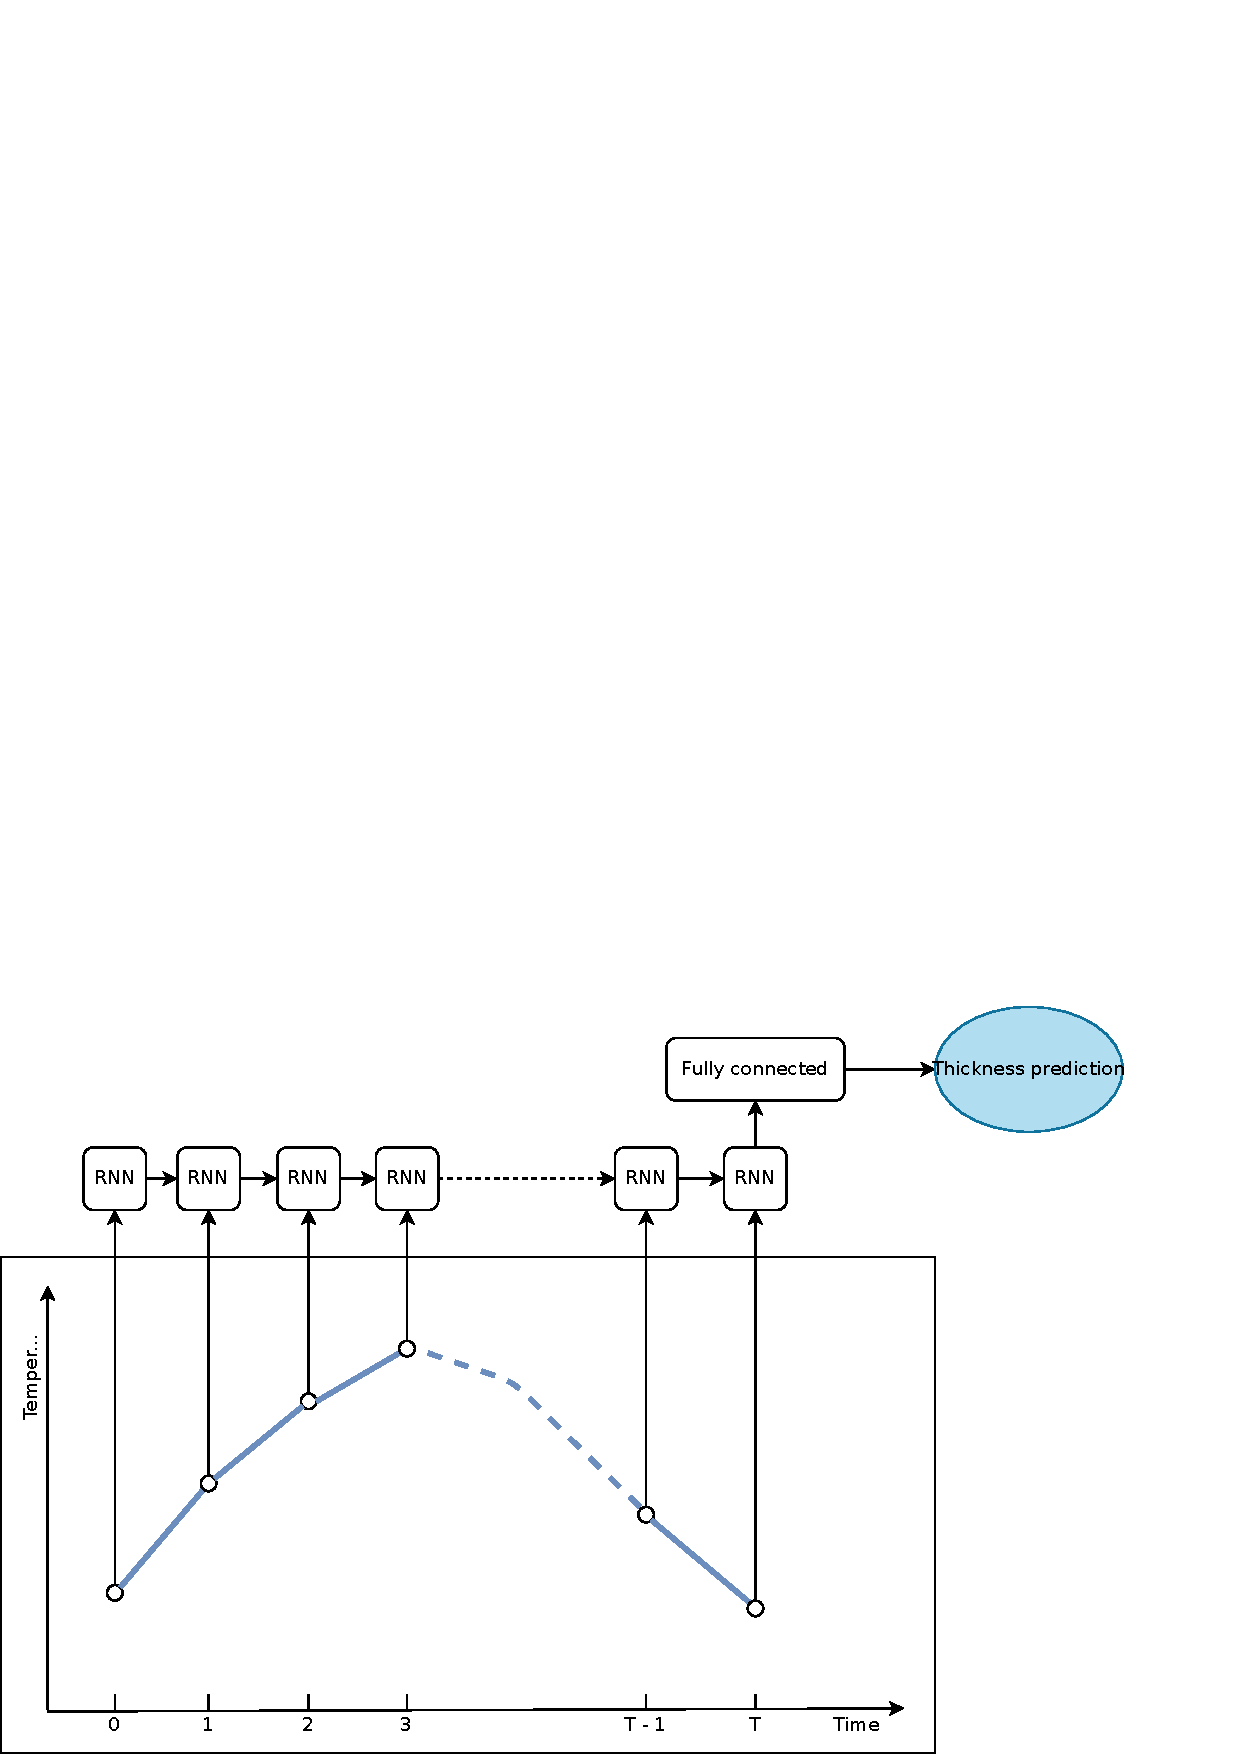
\includegraphics[scale=0.45]{images/chapter_4/rnn_model.png}
\caption{RNN-based model}
\label{fig:rnn_model}
\end{figure}


\subsubsection{Spatial-temporal approach} \label{Spatial-temporal approach}

Compared to the previous approach, the method proposed in this section aims to leverage not only the temporal temperature information, but also the spatial one. Instead of extracting the temperature time series for each critical point of the blow-molded parts we can design an \textit{end-to-end} deep learning architecture able to directly handle the input thermal video. In such a way we should be able to take into consideration not only the surface-temperature evolution of a point but also its position on the spatial dimension. 
% This part should be improved
In this instance, the input dataset
\begin{equation}
    D = \{(X^{i}, Y^{i})\}_{i=1}^{m},
\end{equation}
is a collection of pairs $(X^{i}, Y^{i})$ where $X^{i}$ is the input thermal video with $Y^{i}$ as its corresponding thickness values vector
\begin{equation}
    Y^{i} = [y^{i}_{(x_1, y_1)}, y^{i}_{(x_2, y_2)}, ..., y^{i}_{(x_j, y_j)}, ..., y^{i}_{(x_n, y_n)}].
\end{equation}
The role of the spatial-temporal approach is to approximate the transfer function $\hat{g}$ so that
\begin{equation}
    Y^{i} = \hat{g}(X^{i}, i \in [1, m]) + \epsilon.
\end{equation}
The work presented in this paragraph is largely inspired by the computer vision domain of \textit{Semantic Segmentation}. Semantic image segmentation, or semantic segmentation is the task of clustering the pixels of an image that belong to the same object (or object class). Basically for an input image, semantic segmentation produces a segmentation mask which has the same spatial dimension of the input image where each pixel value correspond to the predicted class. As for other computer vision tasks, state-of-the-art results are obtained through the application of Convolutional Neural Networks (Section \ref{Convolutional Neural Network}).

One popular approach for image segmentation models is to follow an encoder/decoder structure where we “downsample” the spatial resolution of the input, developing lower-resolution feature mappings which are learned to be highly efficient at discriminating between classes, and the “upsample” the feature representations into a full-resolution segmentation map. The encoder-decoder approach, as part of the semantic segmentation domain, was proposed for the first time by \citet{long2015fully} in the Fully Convolutional Network (FCN) architecture and it has been subsequently taken up by other research works \citep{ronneberger2015u,zhao2017pyramid,chen2017rethinking,chen2018encoder,badrinarayanan2017segnet}. The encoder, or contracting path, is, most of the time, a Convolutional Neural Network whose task is to extract features of different spatial resolutions, constituting the so-called “Feature Map”. Compared to the encoder, which reduces the spatial dimension in every layers and increases the channels, the decoder, or expansive path, has the role of restoring the original spatial dimensions by sequentially increasing the spatial dimension while reducing the number of channels. The decoder can be composed of one of multiple decoder block, in the same way the encoder can be more or less deep. Each decoder block computes two different operations: at first it up-sample the feature map using an interpolation method, then it applies a convolutional operation which halves the number of feature channels. Finally, a last convolutional block, sometimes called Segmentation Head, stacked right after the last decoder block produces the segmentation mask.

Instead of predicting a segmentation mask where each pixel belongs to a predefined class, we propose to take advantage of the encoder-decoder architecture to learn reconstructing the thickness of some critical areas of the part. In order to deal with our problem, we have designed an end-to-end pipeline able to provide the critical point values inference given the input video (Figure \ref{fig:proposed_architecture}). 
% The following image will be replaced
\begin{figure}
\centering
\includegraphics[scale=0.45]{images/chapter_4/proposed_architecture.png}
\caption{Proposed architecture (IMAGE WILL BE REPLACED)}
\label{fig:proposed_architecture}
\end{figure}
The proposed pipeline is largely inspired by the encoder-decoder paradigm and in particular to the \textit{Unet} architecture proposed in \citet{ronneberger2015u}. The \textit{Unet} improves the \textit{FCN} architecture by proposing an expansive path which is more or less symmetric to the contracting path that yields a u-shaped architecture. Moreover, the expansive pathway combines the feature and spatial information through a sequence of up-convolutions and concatenations with high-resolution features from the contracting path. By introducing skip connections in the encoder-decoded architecture, fine-grained details can be recovered in the prediction. 
The presented pipeline consists of three main blocks: the spatial encoder, the temporal encoder and the decoder. 

\begin{itemize}
    \item \textit{Spatial Encoder:} The spatial encoder is a CNN which aims to extract the spatial feature map for each frame of the video. The spatial encoder corresponds to the encoder of a traditional encoder-decoder architecture. Compared to the original \textit{Unet} architecture, we replace the original contracting path proposed in the paper with a Residual Network (\ref{Residual Networks}). The ResNet architecture, independently of its depth, it is composed of five main building blocks. Each block sequentially produce lower-resolution feature which will later be used by the decoder to help reconstructing the prediction mask. Given an input thermal video with dimensions $(h, w, c, t)$ where $h$, $w$, $c$ and $t$ are respectively the height of the image, the width, the number of channels and the number of frames of the video sequence. The spatial encoder process each frame $(h, w, c)$ of the input video and it returns a feature maps of size $(h', w', c', t)$ where $h'<<h$, $w'<<w$ and $c'>>c$ and a set of intermediate feature maps.

    \item \textit{Temporal Encoder:} The temporal encoder aims to encode the temporal information of the spatial feature map produced by the spatial encoder. In fact, the spatial encoder encode each frame independently without leveraging any kind of temporal information. In order to encode the temporal information we use a 3D convolutional layers with a kernel size of $(1\times1\times1)$, stacked right after the spatial encoder, which produces a linear projection of the stack of frame-wise feature maps. This projection acts as a dimensional reduction of the temporal dimension. In such a way we are able to produce a new feature map which encode either the spatial and the temporal information. Given the spatial feature map of size $(h', w', c', t)$, the temporal decoder compress the temporal dimension and produces a new \textit{spatial-temporal feature map} with size $(h', w', c', 1)$.  The same convolutional operation, with the same parameters, is applied to compress the temporal information of all the intermediate features maps produced by the spatial encoder.
    
    \item \textit{Decoder:} The decoder projects the discriminative spatial-temporal feature map, to the original input spatial dimension. In the same way as for the \textit{Unet} architecture, intermediate high-resolution features from the encoder path are combined and reused with the upsampled output of each decoder block to help the model reconstructing the prediction mask. The decoder is composed on five decoder blocks and each decoder block applies an upsample operation using the nearest neighbour algorithm followed by two 2D convolutional layers with a kernel size of $3\times 3$, batch normalisation and \textit{ReLu} activation function. A final convolutional layers produce the thickness mask from which the prediction of the critical thickness points are extracted. Given the incoming data of size $(h', w', c', 1)$ the decoder project the encoded pattern to the original spatial dimension producing a 1-channel mask reconstruction $(h, w, 1)$. Given the pixel coordinates of the $n$ critical points, its corresponding thickness prediction can be easily retrieved.
\end{itemize}

Training such an architecture can be a bit more challenging compared to that of the temporal approach because of the number of learnable parameters. Furthermore, we have two main drawbacks:

\begin{itemize}
    \item The size of the training sample is low compared to what is normally used to train this kind of network. For Semantic Segmentation tasks, a dataset of 1000 images is considered small and we hardly would be able to have more than a few hundreds input samples.
    \item The thickness ground-truth map is not known for all the points of the tanks. Semantic Segmentation tasks require, during the training phase of the algorithm, that output mask of the input data is well known. For our problem, the full thickness map of the measured tanks is missing, only a limited number of thickness points are known.
\end{itemize}

The first drawbacks may be potentially handled by applying two different well-known machine learning techniques: \textit{transfer learning} and \textit{data augmentation}. Instead of training a model from scratch, a network with pre-trained parameters may be used as a starting point. Scientific literature suggests that using a pre-trained network would allow to converge faster towards the best solution, especially if the size of the training data is small. Most of the state-of-the-art semantic segmentation approaches make use of pre-trained encoders to start with, while the remaining part of the network is trained from scratch. The use of a pre-trained network is always possible as long the shape of the input data is consistent with the one of the original data used to train the network. 

A second available option to deal with a small dataset would be to make use of the data augmentation technique. Data augmentation in data analysis are techniques used to increase the amount of data by adding slightly modified copies of already existing data or newly created synthetic data from existing data. Popular image augmentation techniques involves geometric transformations such as image flipping, rotation or translation, or colour space transformations. More advanced techniques make use of generative models to create artificial training sample. Regarding our problem, the only augmentation techniques that can be applied are the ones that involves geometric transformation. 
\begin{figure}
\centering
\includegraphics[scale=0.8]{images/chapter_4/data_augmentation.png}
\caption{Image Augmentation}
\label{fig:image_augmentation}
\end{figure}

In fact, since the colour of the image is proportional to the temperature, every augmentation techniques that involves any kind of change in the colour space may completely corrupt the input data.
If the missing of a large volume of input data could be handled with transfer learning and data augmentation, the lack of labelled data in the training dataset may be a little more challenging. In fact, since the full thickness mask of the part is missing, we cannot train the model in classical pixel-wise manner. Traditional semantic segmentation architectures are trained by compute the pixel-wise loss between the ground truth segmentation mask and the reconstruction computed by the network. The computed loss is than back-propagated in the network to adjust the learnable parameters of the architecture. In our particular case, the full thickness ground truth of the part is not known, which means that we cannot compute the pixel-wise loss for all the pixels. It is however still possible to train the network by computing the pixel-wise loss between the mask and the reconstruction only for pixels for which the thickness is known.

\section{Experimental Validation} \label{Experimental Validation}

This section presents the results from a real-world implementation in an industrial case. First, the empirical setting is described as well as the data processing and the training pipeline. Finally we provide the results of this first experimentation.

\subsection{Data collection}

To evaluate the performance of the proposed data-driven model-based quality control, a data acquisition campaign in an industrial environment has been organised. In order to train our models to learn to infer the thickness, given the cooling profile, we need two different types of data: the temperature of the part surface and the thickness measurement of the corresponding part. The Temperature data  has been acquired with an industrial thermal camera OPTRIS PI 640 with a good resolution (640$\times$480), previously calibrated to correctly measure the temperature of the plastic material. Unlike traditional colour images, which are commonly represented using a 3-channel matrix (\textit{RGB}) with 256 different integer values, thermal images collected through the OPTRIS 640 PI are 1-channel matrices where each pixel takes a continuous value corresponding to a temperature in degrees Celsius. Unlike other temperature measuring instruments, the thermal camera has the advantage to evaluate, in a single shot, the temperature of the whole visible surface. Several consecutive shots of the same part make it possible to follow the evolution of the temperature over time (Figure \ref{fig:thermal_video}). 

Before moving forward in the description of the empirical setting, a clarification is needed. Previously, we said that thermal images are 1-channel matrix where each pixel take a continuous value corresponding to a temperature in degree Celsius . Because computers interprets as images only matrix (or 3D tensors) composed of unsigned integers, composed of values ranging from 0 to 255, to display a thermal image is necessary to map the continuous temperatures values to the 0-255 range. In others words, a \textit{colormap} needs to be applied to the raw images in order to display it. In Figure \ref{fig:thermal_video}, as well as for others images of the current chapter, thermal frames are 

\begin{figure}
\centering
\includegraphics[scale=0.55]{images/chapter_4/Thermal_video.png}
\caption{Thermal video $X_i$}
\label{fig:thermal_video}
\end{figure}

Of course, measuring the temperature of the entire surface of the part would require several cameras. As part of the presented experiment, we decided to limit the temperature acquisition to half of the whole surface. The thickness measurement has been carried out on critical points through the use of an ultrasonic measurement instrument routinely used for sampling control. The thickness values of the part selected for our experimentation have typical values ranging between 3 and 10 millimetres. In order to gather comparable data, the image acquisition of each part produced needs to be synchronised with the blowing process in order to synchronise the  acquisition of images on the same relative time. Repeatable mechanical movements of the machine have been used to “trigger” data acquisition. The trigger starts a one minute countdown after which the acquisition of thermal images will begin. This time is mandatory to give the machine the time to unload the part and the machine operator time to place the part in the measuring area. In the experimental context described here, the part is positioned on a table and, at the end of the one minute countdown, the thermal camera starts collecting images. For our experimental measurement campaign, we collected thermal videos on 50 different parts. For each part we recorded 120 consecutive thermal images equally spaced  with a one second interval between one image and the next, for a total of two minutes of data acquisition. For each thermal video, and therefore for each part, we measured 20 critical thickness points evenly distributed on the tank surface (see Figure \ref{fig:critical_points}). 

\begin{figure}
\centering
\includegraphics[scale=1]{images/chapter_4/critical_points.jpg}
\caption{Critical points distribution on the tank surface}
\label{fig:critical_points}
\end{figure}


\subsection{Data processing}

Once the data is collected, some processing operations are needed to prepare data for training. In particular, we need to associate the 20  measured critical thicknesses of the part to their corresponding pixel coordinates on the thermal video. This was done manually, each measured point of the part is identified on the thermal image as a $(x_j, y_j)$ pixel coordinate. Hopefully, since the position of the part does not change during the image acquisition, it is enough to find the pixel coordinates for the first frame. 

Although we can assume that the part does not move during the acquisition, each part is positioned identically with respect to the field of view of the thermal camera. The  $(x_j, y_j)$ coordinates on different thermal videos may therefore refer to different surface areas of the part. In order to align pixel coordinates along parts, a transformation is applied, to each frame, to project the part onto a reference. Before describing the transformation in more detail, we present the \textit{Pinhole camera model}. 

\paragraph{The Pinhole camera model}
The pinhole camera model describes the mathematical relationship between the coordinates of a point in a three-dimensional space and its projection onto a two-dimensional pixel coordinate system. This mathematical relationship depends on the extrinsic and intrinsic parameters of the camera. The extrinsic parameters refer to the rotation matrix and translation vector of the camera coordinate system with regard to the world coordinate system.
Given a point $(x, y, z, 1)^{T}$ in the world coordinate system, we can form its pixel coordinates $(u, v, 1)^{T}$ as follows:
\begin{equation*}
    s\begin{bmatrix} u\\ v\\ 1 \end{bmatrix} = \begin{bmatrix}
        f_x & 0   & c_x\\ 
        0   & f_y & c_y \\ 
        0   & 0   & 1 
        \end{bmatrix}
        \begin{bmatrix}
        r_{11}& r_{12} & r_{13} & t_{x} \\ 
        r_{21}& r_{22} & r_{23} & t_{y} \\
        r_{31}& r_{32} & r_{33} & t_{z}
        \end{bmatrix}
        \begin{bmatrix} x\\ y\\ z \\ 1 \end{bmatrix}
        \enspace,
\end{equation*}
That is:
\begin{equation*}
    s\begin{bmatrix} u\\ v\\ 1 \end{bmatrix} = K[R|T]
    \begin{bmatrix} x\\ y\\ z \\ 1 \end{bmatrix}
        \enspace,
\end{equation*}

where:
\begin{itemize}
    \item $K$ is the 3 $\times$ 3 intrinsic camera matrix.
    \item $f$ is the focal length.
    \item $(u_0,v_0)$ are the coordinates of the principal point at the center of the image plane.
    \item $R$ is the 3 $\times$ 3 rotation matrix.
    \item $T$ is the translation vector.
    
\end{itemize}

Given this  mathematical description, a homography $H$ can be defined as a transformation matrix that maps points from one plane to another. It can be derived by the equation REF:

\begin{equation*}
    \begin{bmatrix} u\\ v\\ 1 \end{bmatrix} = \begin{bmatrix}
        f_x & 0   & c_x\\ 
        0   & f_y & c_y \\ 
        0   & 0   & 1 
        \end{bmatrix}
        \begin{bmatrix}
        r_{11}& r_{12} & r_{13} & t_{x} \\ 
        r_{21}& r_{22} & r_{23} & t_{y} \\
        r_{31}& r_{32} & r_{33} & t_{z}
        \end{bmatrix}
        \begin{bmatrix} u'\\ v'\\ 0 \\ 1 \end{bmatrix}
\end{equation*}

\begin{equation*}
    \begin{bmatrix} u\\ v\\ 1 \end{bmatrix} = \begin{bmatrix}
        f_x & 0   & c_x\\ 
        0   & f_y & c_y \\ 
        0   & 0   & 1 
        \end{bmatrix}
        \begin{bmatrix}
        r_{11}& r_{12} & t_{x} \\ 
        r_{21}& r_{22} & t_{y} \\
        r_{31}& r_{32} & t_{z}
        \end{bmatrix}
        \begin{bmatrix} u'\\ v'\\ 1 \end{bmatrix}
\end{equation*}

\begin{equation*}
    \begin{bmatrix} u\\ v\\ 1 \end{bmatrix} = 
        \begin{bmatrix}
        h_{11}& h_{12} & h_{13} \\ 
        h_{21}& h_{22} & h_{23} \\
        h_{31}& h_{32} & h_{33}
        \end{bmatrix}
        \begin{bmatrix} u'\\ v'\\ 1 \end{bmatrix}
\end{equation*}

\begin{equation} \label{projection}
P=HP'
\end{equation}

where:

\begin{itemize}
    \item $P$ and $P'$ are two points on different planes.
    \item $H$ is a 3 $\times$ 3 matrix composed by intrinsic and extrinsic parameters that relate the two planes together.
\end{itemize}


The mathematical framework presented above can be applied to project all the thermal frames composing the 50 thermal video collected over a reference image. By estimating the homography between the two planes, that of the reference image and that of the image to be projected, each point $P$ of the input image could be projected to the reference image. 

The first frame of each thermal video sequence is used to estimate the homography matrix, through the use of the ORB (Oriented FAST and Rotated BRIEF) algorithm \citep{rublee2011orb}. In a nutshell, ORB is a feature matching algorithm that allows to automatically find some key-points in an image. The ORB algorithm takes as inputs two images, a reference and the one we want to project on this reference, and features that can be matched in the two images are used to estimate the homography matrix. Once the homography is computed, it is applied to map all the pixels of the second image to the pixel of the reference image. The same transformation can then be applied to all the frames in the video sequence, provided that both the camera and the tank are motionless. 
%
Then, depending on the used method, between the functional, temporal and the spatial-temporal, extra processing is needed to prepare data for training.

\subsubsection{Functional approach}
The Functional approach makes use of the temperature time series extracted from the thermal video sequences to infer the corresponding thickness. Given the coordinates $(x_j, y_j)$ of the 20 critical thickness values, it is simple to retrieve the temperature time series by simply collecting the temperature of the coordinate for each sequential frame of the thermal video. By extracting all temperature time series for each critical point of the 50 parts considered, we can build a new time series dataset composed of 1000 (50 x 20) time series and the corresponding thickness values. The time series are then approximated by their parametric expansion. As explained in Section \ref{Functional approach}, three different parametric functions have been identified as good candidates for approximating the pixel-wise temperature surface decay. In order to identify the parametric expansion that best fits the input time series, each expansion was applied to the time-series of the training set. The root mean square error (RMSE) of the overall reconstruction is used to select the best expansion. 

Table \ref{tab:curve_fitting_error} shows the average  RMSE reconstruction for the three parametric expansions considered. The polynomial expansion minimises the reconstruction error and is thus used to summarise the raw time series. 
For each time series, the three parameters defining the second-order polynomial approximation constitute the predictor of the machine learning model.

\begin{table}
\centering
\begin{tabular}{|l|l|}
\hline
Parametric function    & RMSE (train) \\ \hline
Power Law              & 0.29         \\ \hline
Logarithmic            & 0.27         \\ \hline
Polynomial (2° degree) & 0.03         \\ \hline
\end{tabular}
\caption{Curve fitting reconstruction error}
\label{tab:curve_fitting_error}
\end{table}


\subsubsection{Temporal approach}

As for the functional approach, the Temporal approach makes use of the temperature time series extracted from the thermal video sequences to infer the corresponding thickness. Given the coordinates $(x_j, y_j)$ of the 20 critical thickness values, it is simple to retrieve the temperature time series by simply collecting the temperature of the coordinate for each sequential frame of the thermal video. Unlike the previous approach, no extra data processing is required because the raw time series constitute the input data of the RNN model. 

\subsubsection{Spatial-Temporal approach}
Compared to the temporal approach, the spatial-temporal approach also leverages the spatial information contained in the video. It does not require to rearrange the input thermal video in another data structure, but some processing operations are still needed to allow the usage of a pre-trained spatial encoder. In order to be consistent with the data of the \textit{ImageNet} dataset \citep{deng2009imagenet} that was used  to pre-train the network, each thermal frame is converted to a 3-channel RGB image. The maximum and minimum temperatures among all frames are retrieved and the same colormap is applied on all thermal frames of each video sequence. The colormap is the one applied to visualise the thermal frames in the current Chapter. All values are then rescaled in $[0, 1]$ and then normalized using the default mean and standard deviation value of the \textit{ImageNet} dataset.

\subsection{Training}

In this section our training pipeline is presented. For each approach, the data was divided into three sets: the training set (data from 38 parts), the validation set (data from 8 parts) and the test set (data from 5 parts). The training is used to train the model, the validation set is used to evaluate the performance of our methods for each combination of model hyper-parameters and finally, the test set is used to evaluate the ability of the model to generalise the results obtained on new data. For each proposed approach, a Bayesian optimization of hyper-parameters with the \textit{Tree-structured Parzen Estimator} (TPE) \citep{bergstra2011algorithms} algorithm was used to select the hyper-parameters that minimise the \textit{Mean Squared Error} (MSE) on the validation set. The TPE sequentially selects the new hyper-parameters to be tested, thus avoiding an exhaustive grid search, which is quickly too demanding in terms of computing resources.

\subsubsection{Functional approach}

As explained previously, a second-degree polynomial is fitted over the time series to compress the input data in a few features corresponding to the coefficients of the polynomial expansion of the thermal signal. Three machine learning algorithms were compared to model the relationship between the polynomial coefficients and the corresponding thickness values: \textit{Lasso} (linear) regression, \textit{random forest} and \textit{Support Vector Machine} (linear or kernelized) regression. For all models,  hyper-parameters have been optimised by the TPE algorithm (See Section \ref{TPE approach}). 
%Every combination of hyper-parameter values is tested to find the one that minimize the cost function.
%
The exhaustive list of model hyper-parameters and their search space is summarized in Table \ref{tab:functional_search_space}.

\begin{table}
\centering
\label{tab:functional_search_space}
\caption{Hyper-parameter search space for the functional models}
\begin{tabular}{lll} 
\toprule
\textbf{Model}                            & \textbf{Hyper-parameter} & \textbf{Search space}                          \\ 
\midrule
Lasso                                     & $\lambda$                & LogSpace($10^{-5}$, 1)                          \\ 
\midrule
SVM  & Kernel                   & \{Linear, Polynomial, RBF\}  \\ 
\cline{2-3}
                                          & $C$                        & LogSpace($10^{-6}$, 1)                          \\ 
\midrule
\multirow{3}{*}{Random Forest}  & Number of estimators     & {[}50, 51, 52, ..., 500]                       \\ 
\cline{2-3}
                                          & Maximum tree depth       & {[}4, 5, 6, ..., 50]                           \\ 
\cline{2-3}
                                          & Minimum samples leaf     & {[}1, 2, 3, ..., 60]                           \\
\bottomrule
\end{tabular}
\end{table}


\iffalse
\begin{table}
\centering
\begin{tabular}{|l|l|p{5cm}|} 
\hline
\multicolumn{3}{|c|}{Functional approach: model hyper-parameters search space}                                                 \\ 
\hline
\textbf{Model}                            & \textbf{Hyper-parameter} & \textbf{Search space}                          \\ 
\hline
Lasso                                     & $\lambda$                & LogSpace($10^{-5}$, 1)                          \\ 
\hline
\multirow{2}{*}{Support Vector Regressor} & Kernel                   & {[}Linear, Polynomial, Radial basis function]  \\ 
\cline{2-3}
                                          & $C$                        & LogSpace($10^{-6}$, 1)                          \\ 
\hline
\multirow{3}{*}{Random Forest Regressor}  & Number of estimators     & {[}50, 51, 52, ..., 500]                       \\ 
\cline{2-3}
                                          & Maximum tree depth       & {[}4, 5, 6, ..., 50]                           \\ 
\cline{2-3}
                                          & Minimum samples leaf     & {[}1, 2, 3, ..., 60]                           \\
\hline
\end{tabular}

\caption{Functional model search space}
\label{tab:functional_search_space}
\end{table}
\fi

\subsubsection{Temporal approach}
We compared the performance of three RNN-based models: a vanilla RNN, an LSTM and finally a GRU network. The number of hidden units of each computational cell, as well as the number of stacked layers are hyper-parameters that are optimised. A comprehensive summary of the search space for the hyper-parameters is available in Table \ref{tab:rnn_search_space}. 

\begin{table}
    \centering
    \begin{tabular}{|p{3cm}|p{4cm}| }
    \hline
    \multicolumn{2}{|c|}{Temporal approach: model hyper-parameters search space} \\
    \hline
    RNN Cell type & [RNN, LSTM, GRU] \\
    \hline
    N° hidden unit & [8, 16, 32] \\
    \hline
    N° stacked layers & [1, 2] \\
    \hline
    \end{tabular}
    \caption{Temporal approach: model hyper-parameters search space}
    \label{tab:rnn_search_space}
\end{table}
Each model has been trained to minimise the mean squared error metric using the  \textit{Adam} optimiser~\citep{kingma2014adam} with $\beta_{1} = 0.9$, $\beta_{2} = 0.98$ and $\epsilon = 10^{-9}$ and a learning rate sampled by the TPE algorithm on a logarithmic scale,  from $10^{-7}$ to $10^{-2}$. 

\subsubsection{Spatial-Temporal approach}
As for the previous approach, we compared different model configurations on two pre-trained networks: a ResNet18 (18 layers) and a ResNet34 (34 layers). Deeper architectures exist, but we made the choice to limit the search space to the two smaller ResNet architectures because of the limited number of samples in our training set. In fact, deeper architectures allow to extract more complex data representations at the expense of a greater number of parameters and increased computation time. We claim that ResNet18 and ResNet34 are powerful enough to produce a discriminant representation. Another hyper-parameters of the presented architecture is the number of encoder, and decoder, blocks. As stated in section \ref{Residual Networks}, all ResNet architectures, independently on their depths, have 5 main convolutional blocks. Actually, it is possible to slightly change the architecture in order to stop the encoding computation before the last block. This allows to reduce the complexity of the architecture and thus prevent possible over-fitting problems. For instance, we could take into account only the first 3 convolutional building blocks of the ResNet in such a way that the output of the third convolutional building block would be the spatial feature map and the output of the first and second blocks would be the intermediate encoded features. Since the encoder and decoder are symmetrical, reducing the number of encoder blocks also implies a reduction in the number of decoder blocks.

\begin{table}[h!]
    \centering
    \begin{tabular}{|p{3cm}|p{4cm}| }
    \hline
    \multicolumn{2}{|c|}{Spatial-Temporal approach: model hyper-parameters search space} \\
    \hline
    Encoder & [ResNet18, ResNet34] \\
    \hline
    N° of blocks  & [3, 4, 5] \\
    \hline
    \end{tabular}
    \caption{Spatial-Temporal approach: model hyper-parameters search space}
    \label{tab:spatial_temporal_search_space}
\end{table}

% Talk about different loss function
As for the Temporal approach, each model configuration has been trained to minimise the MSE metric using \textit{Adam} optimiser with $\beta_{1} = 0.9$, $\beta_{2} = 0.98$ and $\epsilon = 10^{-9}$ and a learning rate sampled by the TPE algorithm on a logarithmic scale from $10^{-10}$ to $10^{-2}$. 

\subsection{Results}

In this section the results obtained with the three approaches are presented and compared. Performances are measured using the Root Mean Squared Error (RMSE), which has the benefit of penalising large errors and whose value is easy to interpret because it has the same unit as the dependent variable. This means that all the scores presented below represent the average thickness reconstruction error in millimetres.

For the functional approach, random forest performs better in both fit on the training set and generalization on the test set (Table \ref{tab:functional_model_results}).
%
\begin{table}[h!]
    \centering
    \begin{tabular}{|l|p{2.8cm}|p{2.8cm}|p{2.8cm}|}
    \hline
    \multicolumn{4}{|c|}{Functional approach: best model} \\
    \hline
    Model & RMSE train  & RMSE validation  & RMSE test  \\
    \hline
    Lasso & \textbf{0.95} & \textbf{0.91} & \textbf{0.89} \\
    \hline
    Support Vector Regressor & \textbf{0.80} & \textbf{0.73} & \textbf{0.76} \\
    \hline
    Random Forest Regressor & \textbf{0.19} & \textbf{0.54} & \textbf{0.48} \\
    \hline
    \end{tabular}
    \caption{Functional model results}
    \label{tab:functional_model_results}
\end{table}
%
The error is about 0.5 mm, which is not totally satisfactory from an industrial point of view. However, this first experiment allowed us to demonstrate that there is a relationship between the temperature evolution of a zone of the part and the corresponding thickness, as assumed in  Section \ref{Motivation}.

\begin{figure}
\centering
\includegraphics[scale=0.48]{images/chapter_4/temporal_scatter.png}
\caption{Prediction \textit{versus} ground truth scatter plots in train (left) and test (right) for the functional approach based on random forest regression}
\label{fig:gt_prediction_functional}
\end{figure}

Figure \ref{fig:gt_prediction_functional} shows the scatter plots of the predicted thickness and ground-truth thickness for the training set and the test set. The plots confirm the ability of the modef to distinguish between large and small thicknesses. Moreover, they show that the model is more accurate for thin points  (close to 3 mm). This observation is encouraging because the thinnest points are also the most critical to ensure that the part meets the customer's specifications.

Among all temporal trained model, the configuration that minimises the validation error is a GRU model with 8 hidden units per cell and one layer. The results obtained are summarised in Table \ref{tab:temporal_model_results}.
%
\begin{table}
    \centering
    \begin{tabular}{|p{3.2cm}|p{3.2cm}|p{3.2cm}|p{3.2cm}|}
    \hline
    \multicolumn{4}{|c|}{Temporal method: best model} \\
    \hline
    Model & RMSE train  & RMSE validation  & RMSE test  \\
    \hline
    GRU & \textbf{0.54} & \textbf{0.56} & \textbf{0.55} \\
    \hline
    \end{tabular}
    \caption{Temporal model results}
    \label{tab:temporal_model_results}
\end{table}
%
These results are similar to those obtained with random forest, but random forest has a slightly lower error than GRU. Moreover, the computation time needed to train the random forest is significantly lower and it does not require dedicated hardware (GPU). The functional approach therefore seems preferable in all respects. This is confirmed in Figure~\ref{fig:gt_prediction_temporal}, where the functional approach outperforms the temporal approach over all thickness ranges.
\begin{figure}
\centering
\includegraphics[scale=0.48]{images/chapter_4/gt_temporal.eps}
\caption{Prediction \textit{versus} ground truth scatter plots in train (left) and test (right) for the temporal approach based on GRU}
\label{fig:gt_prediction_temporal}
\end{figure}

The third approach (Table \ref{tab:spatial_temporal_model_results}) completely outperforms the previous ones. The best results are obtained using a pre-trained ResNet34 encoder with 5 encoder-decoder blocks, which achieves an RMSE of 0.16 mm on the test set, which is about one-third of the error of the previous approaches. An error of the order of 0.2mm is considered extremely interesting in our industrial context. 
\begin{table}
    \centering
    \begin{tabular}{|p{3.5cm}|p{3.2cm}|p{3.2cm}|p{2.8cm}|}
    \hline
    \multicolumn{4}{|c|}{Spatial-Temporal method: best model} \\
    \hline
    Model & RMSE train  & RMSE validation  & RMSE test  \\
    \hline
    ResNet34-5 blocks) & \textbf{0.14} & \textbf{0.18} & \textbf{0.16} \\
    \hline
    \end{tabular}
    \caption{Spatial-Temporal model results}
    \label{tab:spatial_temporal_model_results}
\end{table}
Figure~\ref{fig:gt_prediction_spatial_temporal} shows that the greatest benefits over the functional approach are at higher thicknesses, but the improvement is already visible at only 4 mm.

\begin{figure}
\centering
\includegraphics[scale=0.48]{images/chapter_4/gt_spatial_temporal.eps}
\caption{Prediction \textit{versus} ground truth scatter plots in train (left) and test (right) for the spatial-temporal approach based on ResNet34}
\label{fig:gt_prediction_spatial_temporal}
\end{figure}

\subsection{Model performance on unseen data point}

% This section should be improved

The results presented in the previous section highlighted the ability of the spatial-temporal model to correctly estimate thicknesses at the critical points of the part.  It is questionable whether the model is able to generalise what it learned for a limited set of critical points to the entire surface of the part. The Spatial-Temporal architecture has been designed to provide, as output, the thickness reconstruction for all the pixels belonging to the tank surface. An example of reconstruction of the thickness mask, produced by the Spatial-temporal architecture, is visible in Figure \ref{fig:thickness_mask_reconstruction}. This figure represents the thickness reconstruction of a random sample belonging to the test set. Unlike the previous images, this time the intensity of the colour is not related to the temperature of the tank, but represents its thickness.
The Figure highlights the ability of the model to produce a thickness reconstruction for all the points belonging to the part surface. However, it struggles to reconstruct some areas, especially those close to the edge of the tank. The ability to predict sensible thicknesses outside the critical points is questionable.

\begin{figure}
\centering
\includegraphics[scale=0.90]{images/chapter_4/mask_reconstruction.png}
\caption{Thickness mask reconstruction example}
\label{fig:thickness_mask_reconstruction}
\end{figure}

In order to test this ability, we modified the validation strategy. Since the entire thickness mask is not available, we used only a subset of the 20 critical thickness values to train the model, reserving the others to compute the prediction error. %Unfortunately, we cannot remove too many points because, in that case, we would deprive the model of too much information.
We removed 4 out of 20 critical points and trained the model on the remaining points. The 4 points removed are then  used to evaluate the ability of the model to predict the thickness outside the critical points. This operation was repeated 20 times by randomly selecting the 4 removed points. In this way, it is possible to evaluate the results on a larger set, composed of $4\times20$ samples.
For each iteration of the algorithm, the same architecture and the same hyper-parameters are used. Results are presented in Figure \ref{fig:gt_prediction_unseen} that shows a positive correlation between ground truth and prediction. 
%
% Should I add a pseudo-code to explain the validation strategy ? 

\begin{figure}
\centering
\includegraphics[scale=0.90]{images/chapter_4/unseen_point_scatter.png}
\caption{Prediction \textit{versus} ground truth scatter plots for the spatial-temporal approach based on ResNet34 on points not seen in training}
\label{fig:gt_prediction_unseen}
\end{figure}
%
However, the prediction of the thickness of unseen points is nowhere near as good as the prediction on unseen parts, and our approach does not meet the industrial requirements in this respect: our model is not reliable when it comes to predicting the thickness of the entire part. In Chapter \ref{Contributions and perspectives} we will present some of the research perspectives we are working on to improve the ability of the model to correctly predict the thickness of the full visible surface. 

\section{Conclusion}

Traditional quality control methods for measuring blow-molded part thickness involves time-consuming operations that cannot be applied online for a 100\% quality inspection. This chapter proposes a new data-driven approach for measuring in real-time the part thickness by leveraging the surface-temperature decay over time. Three different pipelines have been designed to model the relationship between the cooling behavior of a part area, captured through the use of a thermal camera, and the corresponding thickness. The procedure was validated in a real-world manufacturing setting. These results have shown the ability of our method to provide accurate results in predicting thickness values of a set of critical points. Among the three methods presented above, the spatial-temporal approach is the one that achieve the best performance in reconstructing the thickness values of the test set data. 

Future research works would try to generalize what is learned for a limited number of thickness points, in order to potentially reconstruct the full thickness cartography of the whole visible part surface. In Chapter \ref{Contributions and perspectives} we will provide more details about the research perspectives related to this topic. 

\subsection{Scientific Contribution (TO BE COMPLETED)}

This chapter proposes, in our opinion, two mains scientific contributions. At first we have proposed a general framework to improve the control quality of manufactured parts. In particular, we propose to improve the quality control of the manufactured parts by introducing TO BE FINISHED  

Secondly, an application of the current approach in the framework of this thesis project is presented. We have proposed a new approach to infer the thickness of a blow-molded part using a data-driven approach. Three different methods have been proposed. We claims that the same approach could be applied every time that a production process involves TO BE FINISHED

\subsection{Industrial Contribution (TO BE COMPLETED)}

From the industrial point of view, this chapter introduce a new idea of quality control. The traditional Acceptance Sampling approach, used in the industrial context studied, may be enhanced by introducing data-driven model quality control. This approach, which has been proven to be interesting for the task of predicting the thickness of the parts, may be extended to others quality characteristics. Moreover, this approach could also be extended to others process such us the \textit{Post-Cooling}, the \textit{Finishing} or the \textit{Assembly}. By adding extra sensors, or camera, or simply by leveraging the process data collected in the PLC of the machines, it could be possible to provide a quality status to the part without any time-consuming or destructive measurement. 

As regarding the thickness prediction, results are considered accurate enough to move towards the industrialization of the proposed system. In order to industrialize the proposed system, we should be able to take into account extra information such us the temperature of the environment where the machine is located, as well as the temperature of the molds. In fact, the surface temperature of the blow-molded part depends on the ability of the molds to absorb the heat. If the heat absorption capacity changes, as a result of the change in temperature of the molds coolant, the tank surface temperature will be different and the data-driven model accuracy would drop. In the same way, the plant temperature may influence the cooling behavior of the blow-molded part   






\backmatter

\chapter*{Conclusion TO BE FINISHED}
\addcontentsline{toc}{chapter}{Conclusion}
\thispagestyle{empty}

The future direction of the manufacturing industry is to transform industrial processes and products, moving from the reliance on experience-based decision making towards data-centric or evidence-based decision making. It is through this process that Machine Learning will play a major role to advance the digitisation of traditional industrial systems. Plastic Omnium Clean Energy System aims to leverage the Industry 4.0 paradigm in order to keep its leadership in the manufacturing industry of fuel tanks. For Plastic Omnium, the Industry 4.0 paradigm can provide a new way of looking at performance, with a more precise and immediate vision (based on real-time indicators) of the entire production chain, but also the optimisation of production through the use of data-driven methods. Plastic Omnium identifies four majors pillars driving the fourth industrial revolution: \textit{Smart Factories}, \textit{Digital Industrialisation}, \textit{Predictive Quality} and \textit{Predictive Maintenance}. In this research work we have focused in the \textit{Predictive Quality} pillar. In particular, we have demonstrated how machine learning can contribute to a process of continuous quality improvement. Internally collected plant data, as well as new sources of data coming from new sensors may be leveraged through a machine learning data-driven method to model the relationship between the input process data and the output quality data. We claims that the improvement of the overall quality of a production line can be obtained by working either on the process and either on the quality control. This for us definitely makes sense as the production of a part compliant with the specifications is the result of a careful work in optimising the production process, as well as the ability to quickly identify a deviation in the quality of the finished part. By quickly identifying a quality problem it is possible to react faster and adjust the process, limiting the production of non-conforming parts.
% Chapter 1 DONE
Our dissertation has developed as follow. In chapter 1, we have emphasised the importance of the ever growing amount of data available in the manufacturing plants. These data could be used to discover hidden patterns, through machine learning, and to bring value to the overall production chain. Subsequently, the industrial context of the extrusion blow-moulding is presented. extrusion blow-moulding is a complex manufacturing process which consists of two sub-processes: the extrusion and the blow-moulding. The high degree of freedoms of this manufacturing process is captured by a large amount of process parameters which allows to define the process status at a given instant in time. Fuel tanks produced through this manufacturing process must respect some dimensional and geometrical constraints to ensure the integrity of the part and to comply with the costumer specifications. In order to asses the conformity of the part, thickness measurement are routinely performed. Measuring the thickness in real-time is a time-consuming task that cannot be done online. For that reason, only certain parts of the entire production batch are measured. Historically, the weight of the tank is used as an alternative of the thickness to asses that the plastic shell is composed to sufficient material to ensure its robustness. Compared to thickness, the tank weight is easily measurable inline. A literature review targeting the Quality improvement domain in the extrusion blow-moulding has been conducted to evaluate previous works and to define the starting point of our research work. The bibliographical research has highlighted that most of the the previous works leverage data-driven methods to try to characterise the quality variability given some input process data. Due to the complexity of the manufacturing process data-driven methods has proven to be preferable compared to expertise-based methods . Because of this, we have decided to direct our research work towards the data-driven methods.
% Chapter 2 DONE
In chapter 2, we described a general data-driven framework that can be used to leverage past manufacturing data to try to improve the quality of the produced parts. This approach is composed of four main stages: data collection, data processing, exploratory data analysis and supervised machine learning modelling. We claim that Supervised machine learning approaches are preferable compared to the Unsupervised ones in the context of ours research problem. In fact, we want to approximate the relationship between the input process data and the quality of the part. An unsupervised machine learning approach could be used to detect unstable operating condition in a production process but any connection with the quality part would be missing. Linear models, with or without penalty term, tree-based methods and Support Vector Machines are well known Supervised machine learning algorithm that lend themselves very well to being used with structured data. Deep Learning, a sub-field of machine learning, however, provide the best results when the input data are unstructured. For instance, when dealing with images, videos or time series, Deep Learning often provides better results. However, Deep Learning architectures require a large amount of data to converge towards a stable solution. Transfer learning may partially mitigate this limitation. Instead of training an architecture from scratch, the parameters of a pre-trained model are fine-tuned. 
% Chapter 3 DONE
In chapter 3, we presented a first application of the proposed data-driven method in the context of our industrial use-case. We made the choice of working on the modelling of the weight of the tank given the input process parameters. Building a model able at inferring the weight of the tank would allow for a better comprehension of our industrial process. Process data have been collected and pre-processed. Unfortunately the parison length, considered in literature as one of the key parameter in explaining the dimensional variability of the part was not available. A camera-based system leveraging Deep Learning has been put in place to detect the parison in real-time and to compute its length. The measured length, as well as the the other process parameters, constitute the input data for the Supervised machine learning model. Results has show the impossibility to build a predictive model by highlighting a whole series of difficulties that we have encountered in a context full of uncertainty as the industrial one. In particular, the critical process parameters, historically monitored to control the process, do not provide useful information for predicting the weight of the manufactured products. Some of the possible explanations have been discussed: the non-stationarity of our process and the lack of data about raw material above all. Nonetheless, this research work has enabled us to identify some areas for improvement in the production process. The \textit{SmartBMM} project has started from the observation that most of the scraps occurs in the transient regime when the machine is not yet stable. As a consequence, we have decided to completely automate the way the extrusion blow-moulding machines are started with the main idea to reduce the duration of the transient phase. The project has been subsequently extended to automate and optimise other machine phases such as the Purge ones.
% Chapter 4 DONE
Consequently, we have oriented chapter 4 to present and highlight a solution to infer directly the thickness of the part without relying on the tank weight. Firstly, a simple statistical analysis has demonstrated how the correlation between the weight and the thicknesses of the tank is quite low. This calls into question the effectiveness of using the weight to infer the part conformity. As the weight is not sufficient to guarantee the dimensional conformity of the parts produced, we decided to focus our efforts directly towards the tanks thickness. The proposed method addresses the real-time thickness inference issue by leveraging thermal imaging and machine learning to provide a prediction of the thickness of different critical areas of the part. We have observed that different areas of the part have different cooling behaviours depending on their thickness. Areas with smaller thicknesses cool down faster than those with higher thicknesses. For the thicker zones, the surface temperature even starts to increase before decreasing. This phenomenon is due to the release of energy from the innermost plastic layer that has not be in direct contact with the mould surfaces. This surface temperature decay, easily measured by taking consecutive thermal frames over time, could be leveraged to infer the thickness of the part. Three different data-driven pipelines have been presented. The first one leverages parametric expansions to compress the information of the temperature time series extracted from each critical point. The parameters of the parametric expansions are then fed into a machine learning algorithm. The second pipeline directly exploit the extracted time series by leveraging a recurrent neural network. The third pipeline, which completely outdoes the previous two, directly process the input video without extracting the temperature time series. Finally, we proposed a few directions which appear as promising to extend the thickness reconstruction to others points outside the critical ones. We namely introduced an approach that could be applied in order to reconstruct the entire thickness mask of the part.


\section*{Scientific Contributions}

This research work has in our opinion three main scientific contributions:

\begin{enumerate}
    \item This research work provides to the scientific community an industrial application of machine learning and Deep Learning in the context of the quality improvement. Our research work has made it possible to highlight not only the benefits that machine learning approaches can bring to the manufacturing production chain but also some of the possible issues we can encounter when such a methods are applied in a real industrial context. 
    
    \item We provide a new approach for measuring the thickness in real-time in a non-contact manner. Our approach relays in Deep Learning and thermal imaging to infer the thickness of a blow-moulded fuel tank. Thermal imaging for inferring the thickness of an object is not a new idea but, at our knowledge, this is the first time that a data-driven method has been leveraged to infer the thickness given the surface decay temperature. We claim that such an approach could be extended to others manufacturing production processes where the manufactured part undergoes a cooling process.    
    
    \item We have shown how Deep Learning could be leveraged in the manufacturing industry even if the amount of data available is limited. Transfer learning and data augmentation have proven to be effective techniques to address the data scarcity issue.  

\end{enumerate}


\section*{Industrial Contributions}

This research work has in our opinion five main industrial contributions:

\begin{enumerate}
    %OK
    \item We provide to the company a general framework for dealing with quality improvement topics in a data-driven manner. This approach open ups new possibilities in term of quality control and process improvement. In this PhD dissertation, we have shown an application of such a framework in the context of the extrusion blow-moulding but, the same approach could be extended to others production processes. For instance, such a framework is currently used in the finishing centres of the production line to asses the quality of the welding parts.
    %OK
    \item Results presented all along this research work allow to call into questions some of the previous beliefs about the functioning of the extrusion blow-Moulding process. The critical process parameters, as they are collected today, are not enough to explain the part weight variability. Moreover, the weight has proven to not be sufficient to ensure the correct material distribution. 
    %OK
    \item The \textit{SmartBMM} software is currently in deployment in all the manufacturing plants of the company. The daily usage in the pilot plants, where the solution has been developed, shows a significant reduction in Purge cycles times as well in the starting phases. Moreover, by reducing the transient regime duration we are able to indirectly reduce the part non-conformities.
    % OK
    \item The parison length measurement in real time provides interesting information about the process. A few initiatives are currently in progress to leverage the real-time parison length measurement to adjust the die-gap opening accordingly to the length of the parison. This would allow for a better repeatability of the material distribution over the parison length. 
    %OK
    \item We propose an approach to infer the thickness of blow-moulded parts using thermal imaging and a Deep Learning without any direct measurement of the part. Results are considered accurate enough to move towards the industrialisation of the proposed system. Such an approach would allow for a 100\% thickness part inspection.   

\end{enumerate}

\section*{Perspectives}

Finally, we would like to draw attention on a few perspective research directions. These questions appear essential given our current understanding of the manufacturing industry and the state of the machine learning research. In our opinion, there are three majors challenges to overcome for the manufacturing industry, in order to properly apply machine learning models in production: machine learning model uncertainty management and the machine learning life-cycle management. These topics have to be addressed in order to answer the third research objectives presented in the first chapter (see section \ref{Research objectives and methodology}).   
% MODEL UNCERTAINTY
If we want to employ machine learning technology to control the functioning of a production process, or to asses the quality of a manufactured part, we must be extremely cautious about mission-critical tasks, which necessitates not just advancements in model and algorithm accuracy, but also security limits and uncertainty management in system design. For instance, for a manufacturing company with low percentage of quality scraps, a machine learning model with a 80\% accuracy in prediction may lead to incorrect alerts. Non detecting non-conforming parts, or even worst, declaring a part as non compliant when in fact it is fully compliant, is surely a problem for the company. 
The experimentation conducted during this research work have highlighted how it is extremely hard to build a robust machine learning algorithm in the context of our manufacturing process. We claim that a 100\% model accuracy is utopistic in our industrial context but in general in the manufacturing industry. Therefore, future works may focus on how a model with a limited accuracy could provide values to a company. Maybe the accuracy is not enough to automatically declare the part as non-conforming inside a traceability system, but it could be used to quickly identify some product quality deviation.

% MODEL LIFE-CYCLE MANAGEMENT
Another topic related to decision-making is the machine learning model life-cycle management. Results presented all along this PhD dissertation have highlighted that the extrusion blow-moulding process is non-stationary. In the manufacturing industry, multiples non controllable factors may lead to a change in the input data distribution. If the input data distribution changes over time, a model would not be able to provide the same accuracy over time. It becomes mandatory to correctly handle the model re-train over time. In order to re-train the model, it becomes extremely important to correctly handle the data acquisition of new quality control data to provides a model FINIRE. morever, future research works could leverage the machin learning field of Domain Adaptation. Domain adaptation is the task of adapting models across domains. This is motivated by the challenge where the test and training datasets fall from different data distributions due to some factor. Domain adaptation aims to build machine learning models that can be generalised into a target domain and dealing with the discrepancy across domain distributions.
% 
% \textbf{A future research question could be}: How to, effectively and automatically, handle the uncertainty of a trained machine learning model in the manufacturing industry? 



% GENERALISATION
Strictly related to the previous topic ...


The last topic that should be addressed is the one of the model generalisation across different machines. A machine learning model trained on a specific machine will not necessarily work for another machine. Some external factors that we do not control may change. The input raw material, 

For instance, the FINIRE 

We claims that transfer learning could be a solution FINIRE


In fact, we claims that a model trained on a specific machine, for a specific product, could not properly generalise FINIRE. This means lots of money and energy is needed to continuously build new trainig data and to train new models for new problems. We think that transfer learning could partially solve such an issue. In fact, FINIRE

What works for a machine will not necessarily work for another machine. Some external factors that we do not control may change. For instance, the FINIRE 


Moreover, what works for a machine will not necessarily work for another machine. 


% 

% non facile nel futuro prossimo ma forse fattibile in un futuro remoto 
we claims that it will be quite difficult to build a genralised modle able to 
% 



\clearpage

\bibliographystyle{apalike}
\bibliography{references}
\addcontentsline{toc}{chapter}{Bibliography}

% Appendix
\appendix
% A
\chapter{Plastic Omnium Clean Energy System} \label{Plastic Omnium}
\markboth{\MakeUppercase{Plastic Omnium Clean Energy System}}{\MakeUppercase{Plastic Omnium Clean Energy System}}


The Clean Energy Systems (CES) is one of the three divisions of the Plastic Omnium company, specialised in plastic fuel tanks systems, and depollution systems, mostly for private and commercial vehicles. In 2018, more than 22M fuel systems have been delivered, representing 1 out of 4 commercialised vehicles equipped with a fuel system coming from the CES division.
The material used for producing the fuel tanks is HDPE (High-Density Polyethylene). There are several reasons why they are made of plastic and not in metal as they used to be (for cars):
\begin{itemize}
    \item Plastic is lighter than metal (about 30\%), which allows a reduction of fuel consumption.
    \item The raw material is less expensive.
    \item A plastic tank cannot explode: it will melt, and the fuel will be spilled on the floor.
\end{itemize}

However, one issue is the permeability: as plastic is a porous material, fuel will eventually end up going through it and that leads to two major issues: the consumer will lose some of his gas, and this one will go into the air and pollute the atmosphere. That is why a fuel tank is not a simple container of fuel: it’s a real part composed of complex technologies, from the production processes to the material used, and also the parts attached to the fuel system: filling system, pump gauge module, ventilation. These are used to make the fuel system (Figure \ref{fig:Fuel System}) less permeable to cope with the different regulations.
\begin{figure}
\centerline{\includegraphics[scale=0.4]{images/appendix_A/fuel_system.png}}
\caption{Fuel System}
\label{fig:Fuel System}
\end{figure}
A fuel system is composed of a fuel tank (Figure \ref{fig:Plastic Fuel Tank}) and a filler pipe (Figure \ref{fig:Filler Pipe}, the latter is the only part visible of the system by the end user, to refill the tank at the station.

\begin{figure}
\centerline{\includegraphics[scale=0.6]{images/appendix_A/Plastic_fuel_tank.png}}
\caption{Plastic Fuel Tank}
\label{fig:Plastic Fuel Tank}
\end{figure}
\begin{figure}
\centerline{\includegraphics[scale=0.6]{images/appendix_A/Filler_pipe.png}}
\caption{Filler Pipe}
\label{fig:Filler Pipe}
\end{figure}

The SCR technology (Selective Catalytic Reduction) is an effective response to the regulatory requirements limiting emissions of nitrogen oxides ($NO_x$) from diesel vehicles. Combining a tank with a pump and gauge module, this system injects vaporised \textit{AdBlue®} into the hot exhaust gases, causing a chemical reaction that transforms $NO_x$ into water vapor. Plastic Omnium CES has developed a range of SCR systems to meet the needs of all types of vehicles, from the smallest European city car to the largest American pickup truck.
% B
\chapter{Fuel system production process} \label{Fuel system production process}
\markboth{\MakeUppercase{Fuel system production process}}{\MakeUppercase{Fuel system production process}}

The manufacturing of a complete fuel system is the result of multiple production stages: 

\begin{itemize}
    \item Material Supply: plastic material is stored in dedicated silos into the plant. The material supply equipment is directly connected to the extrusion blow-moulding machine in order to continuously feed the extruders with new raw material.
    \item Extrusion blow-moulding: it is the core manufacturing process of the entire production line. During this stage raw material is transformed in a hollow fuel tank. 
    \item Post Cooling: once the fuel tank has been blown, it enters a phase of post-mould cooling, where its temperature is lowered a second mould. This operation allows for the stabilisation of the tank dimensions.
    \item Finishing: during the finishing stage the hollow tank is cut in different areas and extra components are welded on it.
    \item Assembly: finally, some parts such as the filler pipe are assembled on the tank and every tank is checked to detect possible leaks.
\end{itemize}

The full process is outlined in Figure \ref{fig:Full_production_process}.

\begin{figure}
\centerline{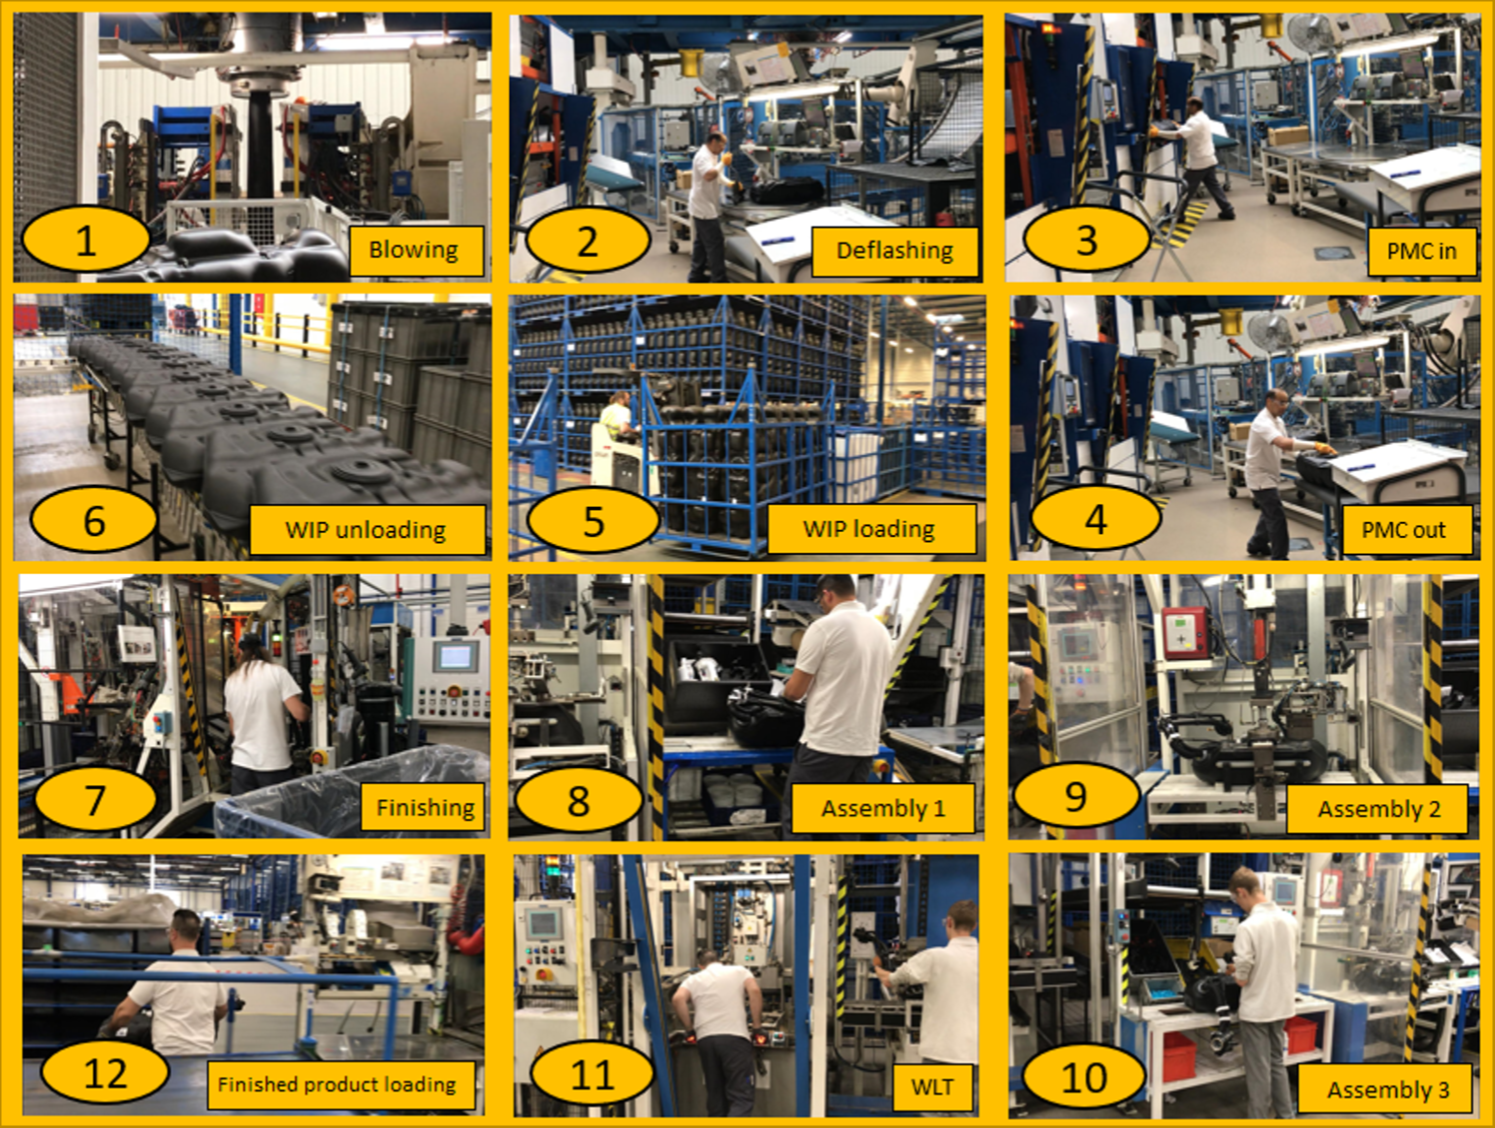
\includegraphics[scale=0.4]{images/appendix_B/Blow_molding_process.png}}
\caption{Full production process}
\label{fig:Full_production_process}
\end{figure}

\end{document}
